% Aalto Master's Thesis template
%TODO : see ITMO template: https://github.com/kitchenknif/ITMOThesisTemplate
% Compatible with: UTF-8, pdflatex, biblatex, biber
%
% Compile using the following commands:
% $ pdflatex thesis.tex
% $ biber thesis
% $ pdflatex thesis.tex
%pdflatex -output-directory=out "\def\IsAalto{yes} 
\documentclass[12pt,a4paper,oneside,pdftex]{report}


\usepackage{subcaption}
\usepackage{graphicx}
\usepackage{amsmath}

\usepackage{tikz}
\usetikzlibrary{positioning}
\usetikzlibrary{calc}
\usetikzlibrary{arrows}
\usetikzlibrary{decorations.pathmorphing,decorations.markings}
\usetikzlibrary{shapes}
\usetikzlibrary{patterns}
\usetikzlibrary{automata}

\tikzset{
c/.style={
  circle,
  inner sep=0pt,
  text width=6mm,
  align=center,
  draw=black,
  fill=white
  }
}


\begin{document}

Hello

\section{Kakashka}
blub

%pdflatex -output-directory=out "\def\IsAalto{yes} 
\documentclass[12pt,a4paper,oneside,pdftex]{report}


\usepackage{subcaption}
\usepackage{graphicx}
\usepackage{amsmath}

\usepackage{tikz}
\usetikzlibrary{positioning}
\usetikzlibrary{calc}
\usetikzlibrary{arrows}
\usetikzlibrary{decorations.pathmorphing,decorations.markings}
\usetikzlibrary{shapes}
\usetikzlibrary{patterns}
\usetikzlibrary{automata}

\tikzset{
c/.style={
  circle,
  inner sep=0pt,
  text width=6mm,
  align=center,
  draw=black,
  fill=white
  }
}


\begin{document}

Hello

\section{Kakashka}
blub

%pdflatex -output-directory=out "\def\IsAalto{yes} 
\documentclass[12pt,a4paper,oneside,pdftex]{report}


\usepackage{subcaption}
\usepackage{graphicx}
\usepackage{amsmath}

\usepackage{tikz}
\usetikzlibrary{positioning}
\usetikzlibrary{calc}
\usetikzlibrary{arrows}
\usetikzlibrary{decorations.pathmorphing,decorations.markings}
\usetikzlibrary{shapes}
\usetikzlibrary{patterns}
\usetikzlibrary{automata}

\tikzset{
c/.style={
  circle,
  inner sep=0pt,
  text width=6mm,
  align=center,
  draw=black,
  fill=white
  }
}


\begin{document}

Hello

\section{Kakashka}
blub

%pdflatex -output-directory=out "\def\IsAalto{yes} \input{test.tex}" 
%pdflatex -output-directory=out "\input{test.tex}" 
\ifdefined\IsAalto
  def
\else
  non-def
\fi

\begin{figure}
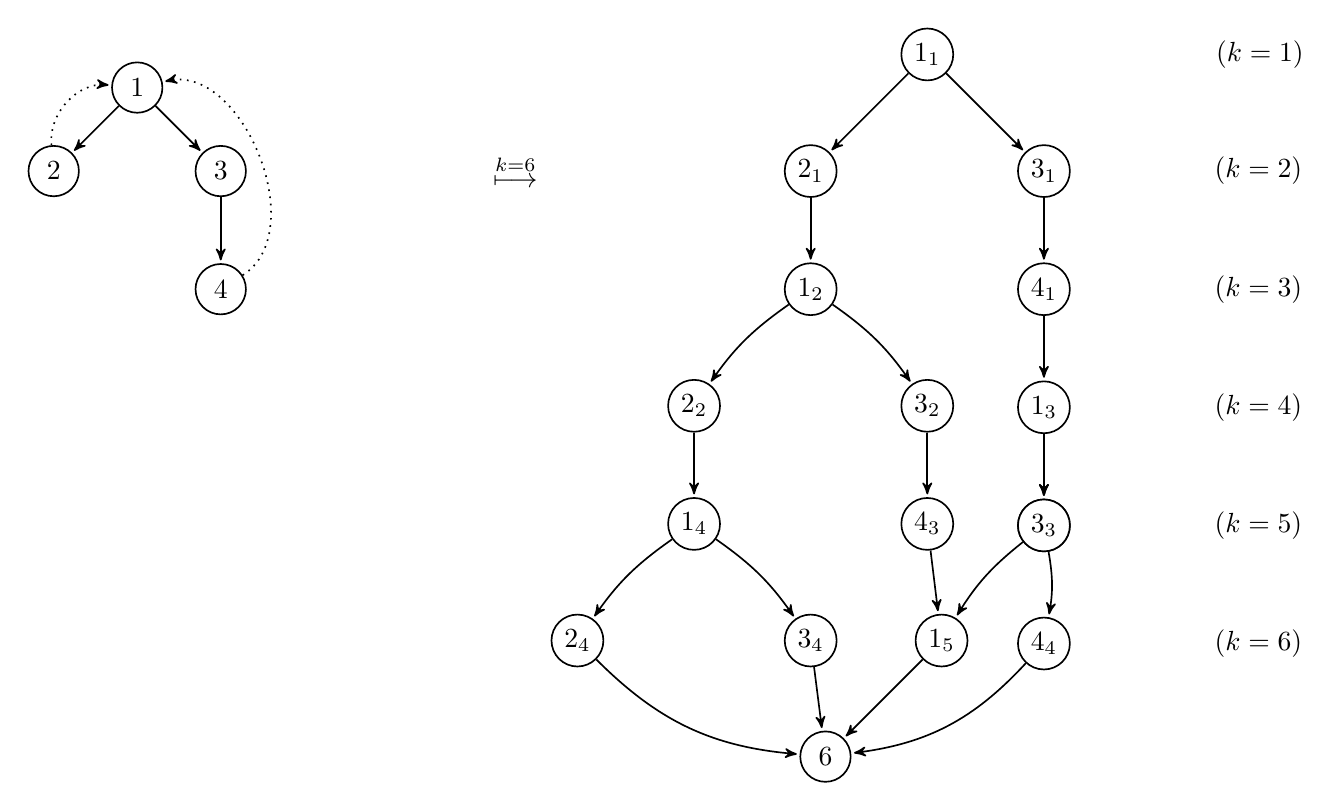
\begin{tikzpicture}[->,>=stealth',shorten >=1pt,auto,node distance=1.5cm,semithick]
\node[c] (1) [] {$1$};
\node[c] (2) [below left of=1] {$2$};
\node[c] (3) [below right of=1] {$3$};
\node[c] (4) [below of=3] {$4$};
\path[->]
(1) edge [] node {} (2)
(2) edge [bend left=50,dotted] node {} (1)
(1) edge [] node {} (3)
(3) edge [] node {} (4)
(4) edge [bend right=80,dotted] node {} (1)
;
\node[draw=none] (impl) [right=3cm of 3] {$\overset{k = 6}{\longmapsto}$};
;
\node[c] (21) [right=3cm of impl] {$2_1$};
\node[c] (11) [above right=1cm and 1cm of 21]{$1_1$};
\node[c] (31) [below right=1cm and 1cm of 11] {$3_1$};
\node[c] (41) [below of=31] {$4_1$};
\node[c] (12) [below of=21] {$1_2$};
\node[c] (22) [below left=1cm and 1cm of 12] {$2_2$};
\node[c] (32) [below right=1cm and 1cm of 12] {$3_2$};
\node[c] (13) [below of=41] {$1_3$};
\node[c] (14) [below of=22] {$1_4$};
\node[c] (43) [below of=32] {$4_3$};
\node[c] (23) [below of=13] {$2_3$};
\node[c] (33) [below of=13] {$3_3$};
\node[c] (24) [below left=1cm and 1cm of 14] {$2_4$};
\node[c] (34) [below right=1cm and 1cm of 14] {$3_4$};
\node[c] (15) [below right=1cm and -0.3cm of 43] {$1_5$};
\node[c] (44) [below of=33] {$4_4$};
\node[c] (6) [below left=1cm and 1cm of 15] {$6$};
\node[] (11k) [right=3.2cm of 11] {$(k = 1)$};
\node[] (31k) [right=1.7cm of 31] {$(k = 2)$};
\node[] (41k) [right=1.7cm of 41] {$(k = 3)$};
\node[] (13k) [right=1.7cm of 13] {$(k = 4)$};
\node[] (33k) [right=1.7cm of 33] {$(k = 5)$};
\node[] (44k) [right=1.7cm of 44] {$(k = 6)$};
\path[->]
(11) edge [] node {} (21)
(11) edge [] node {} (31)
(31) edge [] node {} (41)
(21) edge [] node {} (12)
(12) edge [bend right=10] node {} (22)
(12) edge [bend left=10] node {} (32)
(41) edge [] node {} (13)
(22) edge [] node {} (14)
(32) edge [] node {} (43)
(13) edge [] node {} (23)
(13) edge [] node {} (33)
(14) edge [bend right=10] node {} (24)
(14) edge [bend left=10] node {} (34)
(43) edge [] node {} (15)
(33) edge [bend right=10] node {} (15)
(33) edge [bend left=10] node {} (44)
(24) edge [bend right=20] node {} (6)
(34) edge [] node {} (6)
(15) edge [] node {} (6)
(44) edge [bend left=20] node {} (6)
;
\end{tikzpicture}
\caption{Example of the flow graph from Figure~\ref{fig:merged-loop}, unwinded up to the bound $k = 6$} \label{fig:merged-loop}
\end{figure}

\end{document}

" 
%pdflatex -output-directory=out "
\documentclass[12pt,a4paper,oneside,pdftex]{report}


\usepackage{subcaption}
\usepackage{graphicx}
\usepackage{amsmath}

\usepackage{tikz}
\usetikzlibrary{positioning}
\usetikzlibrary{calc}
\usetikzlibrary{arrows}
\usetikzlibrary{decorations.pathmorphing,decorations.markings}
\usetikzlibrary{shapes}
\usetikzlibrary{patterns}
\usetikzlibrary{automata}

\tikzset{
c/.style={
  circle,
  inner sep=0pt,
  text width=6mm,
  align=center,
  draw=black,
  fill=white
  }
}


\begin{document}

Hello

\section{Kakashka}
blub

%pdflatex -output-directory=out "\def\IsAalto{yes} \input{test.tex}" 
%pdflatex -output-directory=out "\input{test.tex}" 
\ifdefined\IsAalto
  def
\else
  non-def
\fi

\begin{figure}
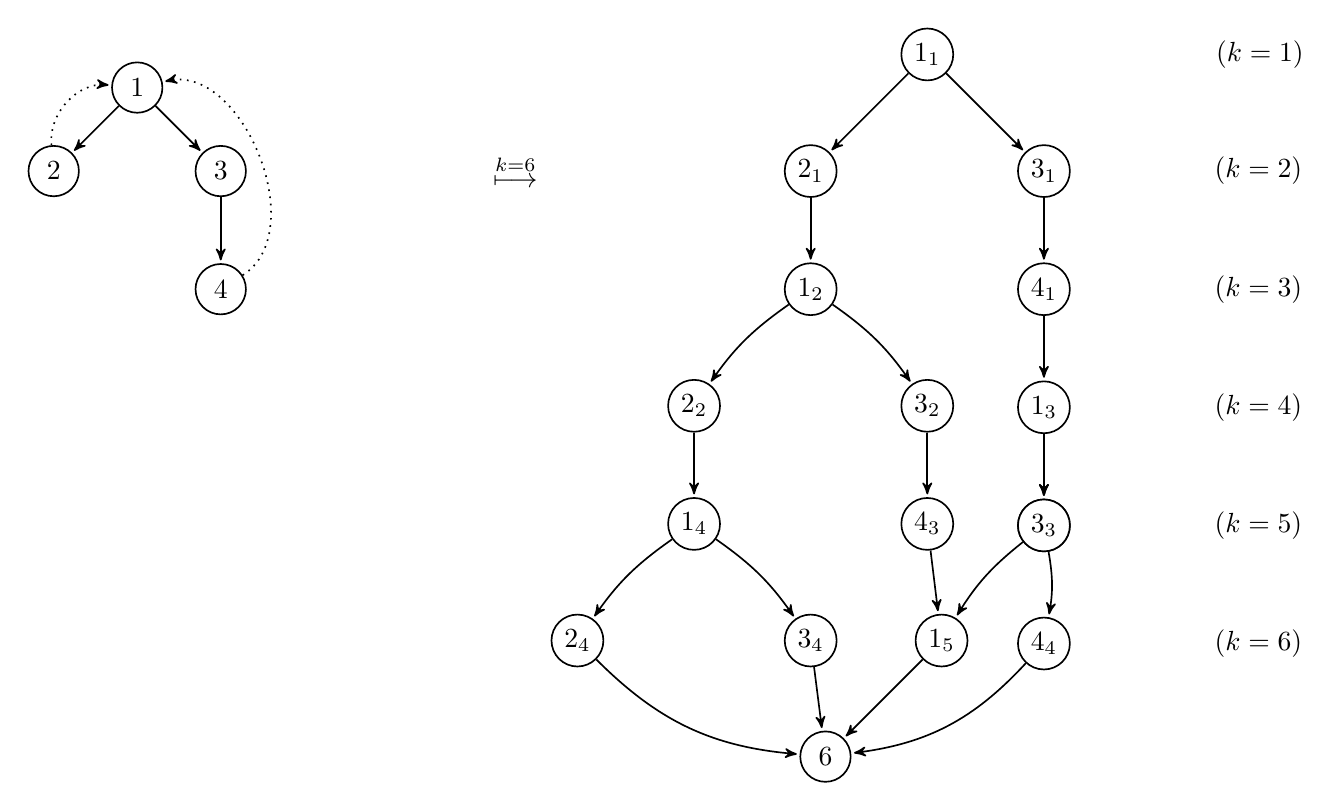
\begin{tikzpicture}[->,>=stealth',shorten >=1pt,auto,node distance=1.5cm,semithick]
\node[c] (1) [] {$1$};
\node[c] (2) [below left of=1] {$2$};
\node[c] (3) [below right of=1] {$3$};
\node[c] (4) [below of=3] {$4$};
\path[->]
(1) edge [] node {} (2)
(2) edge [bend left=50,dotted] node {} (1)
(1) edge [] node {} (3)
(3) edge [] node {} (4)
(4) edge [bend right=80,dotted] node {} (1)
;
\node[draw=none] (impl) [right=3cm of 3] {$\overset{k = 6}{\longmapsto}$};
;
\node[c] (21) [right=3cm of impl] {$2_1$};
\node[c] (11) [above right=1cm and 1cm of 21]{$1_1$};
\node[c] (31) [below right=1cm and 1cm of 11] {$3_1$};
\node[c] (41) [below of=31] {$4_1$};
\node[c] (12) [below of=21] {$1_2$};
\node[c] (22) [below left=1cm and 1cm of 12] {$2_2$};
\node[c] (32) [below right=1cm and 1cm of 12] {$3_2$};
\node[c] (13) [below of=41] {$1_3$};
\node[c] (14) [below of=22] {$1_4$};
\node[c] (43) [below of=32] {$4_3$};
\node[c] (23) [below of=13] {$2_3$};
\node[c] (33) [below of=13] {$3_3$};
\node[c] (24) [below left=1cm and 1cm of 14] {$2_4$};
\node[c] (34) [below right=1cm and 1cm of 14] {$3_4$};
\node[c] (15) [below right=1cm and -0.3cm of 43] {$1_5$};
\node[c] (44) [below of=33] {$4_4$};
\node[c] (6) [below left=1cm and 1cm of 15] {$6$};
\node[] (11k) [right=3.2cm of 11] {$(k = 1)$};
\node[] (31k) [right=1.7cm of 31] {$(k = 2)$};
\node[] (41k) [right=1.7cm of 41] {$(k = 3)$};
\node[] (13k) [right=1.7cm of 13] {$(k = 4)$};
\node[] (33k) [right=1.7cm of 33] {$(k = 5)$};
\node[] (44k) [right=1.7cm of 44] {$(k = 6)$};
\path[->]
(11) edge [] node {} (21)
(11) edge [] node {} (31)
(31) edge [] node {} (41)
(21) edge [] node {} (12)
(12) edge [bend right=10] node {} (22)
(12) edge [bend left=10] node {} (32)
(41) edge [] node {} (13)
(22) edge [] node {} (14)
(32) edge [] node {} (43)
(13) edge [] node {} (23)
(13) edge [] node {} (33)
(14) edge [bend right=10] node {} (24)
(14) edge [bend left=10] node {} (34)
(43) edge [] node {} (15)
(33) edge [bend right=10] node {} (15)
(33) edge [bend left=10] node {} (44)
(24) edge [bend right=20] node {} (6)
(34) edge [] node {} (6)
(15) edge [] node {} (6)
(44) edge [bend left=20] node {} (6)
;
\end{tikzpicture}
\caption{Example of the flow graph from Figure~\ref{fig:merged-loop}, unwinded up to the bound $k = 6$} \label{fig:merged-loop}
\end{figure}

\end{document}

" 
\ifdefined\IsAalto
  def
\else
  non-def
\fi

\begin{figure}
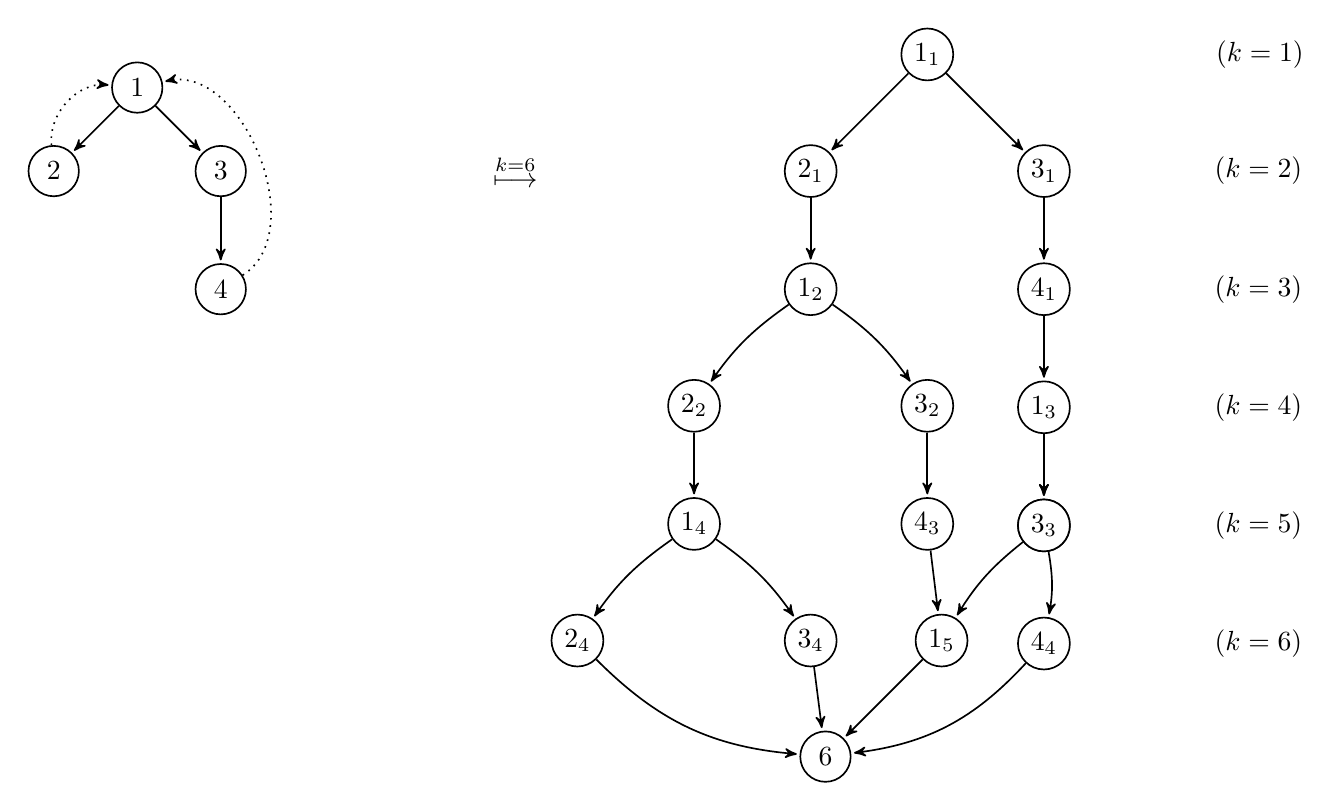
\begin{tikzpicture}[->,>=stealth',shorten >=1pt,auto,node distance=1.5cm,semithick]
\node[c] (1) [] {$1$};
\node[c] (2) [below left of=1] {$2$};
\node[c] (3) [below right of=1] {$3$};
\node[c] (4) [below of=3] {$4$};
\path[->]
(1) edge [] node {} (2)
(2) edge [bend left=50,dotted] node {} (1)
(1) edge [] node {} (3)
(3) edge [] node {} (4)
(4) edge [bend right=80,dotted] node {} (1)
;
\node[draw=none] (impl) [right=3cm of 3] {$\overset{k = 6}{\longmapsto}$};
;
\node[c] (21) [right=3cm of impl] {$2_1$};
\node[c] (11) [above right=1cm and 1cm of 21]{$1_1$};
\node[c] (31) [below right=1cm and 1cm of 11] {$3_1$};
\node[c] (41) [below of=31] {$4_1$};
\node[c] (12) [below of=21] {$1_2$};
\node[c] (22) [below left=1cm and 1cm of 12] {$2_2$};
\node[c] (32) [below right=1cm and 1cm of 12] {$3_2$};
\node[c] (13) [below of=41] {$1_3$};
\node[c] (14) [below of=22] {$1_4$};
\node[c] (43) [below of=32] {$4_3$};
\node[c] (23) [below of=13] {$2_3$};
\node[c] (33) [below of=13] {$3_3$};
\node[c] (24) [below left=1cm and 1cm of 14] {$2_4$};
\node[c] (34) [below right=1cm and 1cm of 14] {$3_4$};
\node[c] (15) [below right=1cm and -0.3cm of 43] {$1_5$};
\node[c] (44) [below of=33] {$4_4$};
\node[c] (6) [below left=1cm and 1cm of 15] {$6$};
\node[] (11k) [right=3.2cm of 11] {$(k = 1)$};
\node[] (31k) [right=1.7cm of 31] {$(k = 2)$};
\node[] (41k) [right=1.7cm of 41] {$(k = 3)$};
\node[] (13k) [right=1.7cm of 13] {$(k = 4)$};
\node[] (33k) [right=1.7cm of 33] {$(k = 5)$};
\node[] (44k) [right=1.7cm of 44] {$(k = 6)$};
\path[->]
(11) edge [] node {} (21)
(11) edge [] node {} (31)
(31) edge [] node {} (41)
(21) edge [] node {} (12)
(12) edge [bend right=10] node {} (22)
(12) edge [bend left=10] node {} (32)
(41) edge [] node {} (13)
(22) edge [] node {} (14)
(32) edge [] node {} (43)
(13) edge [] node {} (23)
(13) edge [] node {} (33)
(14) edge [bend right=10] node {} (24)
(14) edge [bend left=10] node {} (34)
(43) edge [] node {} (15)
(33) edge [bend right=10] node {} (15)
(33) edge [bend left=10] node {} (44)
(24) edge [bend right=20] node {} (6)
(34) edge [] node {} (6)
(15) edge [] node {} (6)
(44) edge [bend left=20] node {} (6)
;
\end{tikzpicture}
\caption{Example of the flow graph from Figure~\ref{fig:merged-loop}, unwinded up to the bound $k = 6$} \label{fig:merged-loop}
\end{figure}

\end{document}

" 
%pdflatex -output-directory=out "
\documentclass[12pt,a4paper,oneside,pdftex]{report}


\usepackage{subcaption}
\usepackage{graphicx}
\usepackage{amsmath}

\usepackage{tikz}
\usetikzlibrary{positioning}
\usetikzlibrary{calc}
\usetikzlibrary{arrows}
\usetikzlibrary{decorations.pathmorphing,decorations.markings}
\usetikzlibrary{shapes}
\usetikzlibrary{patterns}
\usetikzlibrary{automata}

\tikzset{
c/.style={
  circle,
  inner sep=0pt,
  text width=6mm,
  align=center,
  draw=black,
  fill=white
  }
}


\begin{document}

Hello

\section{Kakashka}
blub

%pdflatex -output-directory=out "\def\IsAalto{yes} 
\documentclass[12pt,a4paper,oneside,pdftex]{report}


\usepackage{subcaption}
\usepackage{graphicx}
\usepackage{amsmath}

\usepackage{tikz}
\usetikzlibrary{positioning}
\usetikzlibrary{calc}
\usetikzlibrary{arrows}
\usetikzlibrary{decorations.pathmorphing,decorations.markings}
\usetikzlibrary{shapes}
\usetikzlibrary{patterns}
\usetikzlibrary{automata}

\tikzset{
c/.style={
  circle,
  inner sep=0pt,
  text width=6mm,
  align=center,
  draw=black,
  fill=white
  }
}


\begin{document}

Hello

\section{Kakashka}
blub

%pdflatex -output-directory=out "\def\IsAalto{yes} \input{test.tex}" 
%pdflatex -output-directory=out "\input{test.tex}" 
\ifdefined\IsAalto
  def
\else
  non-def
\fi

\begin{figure}
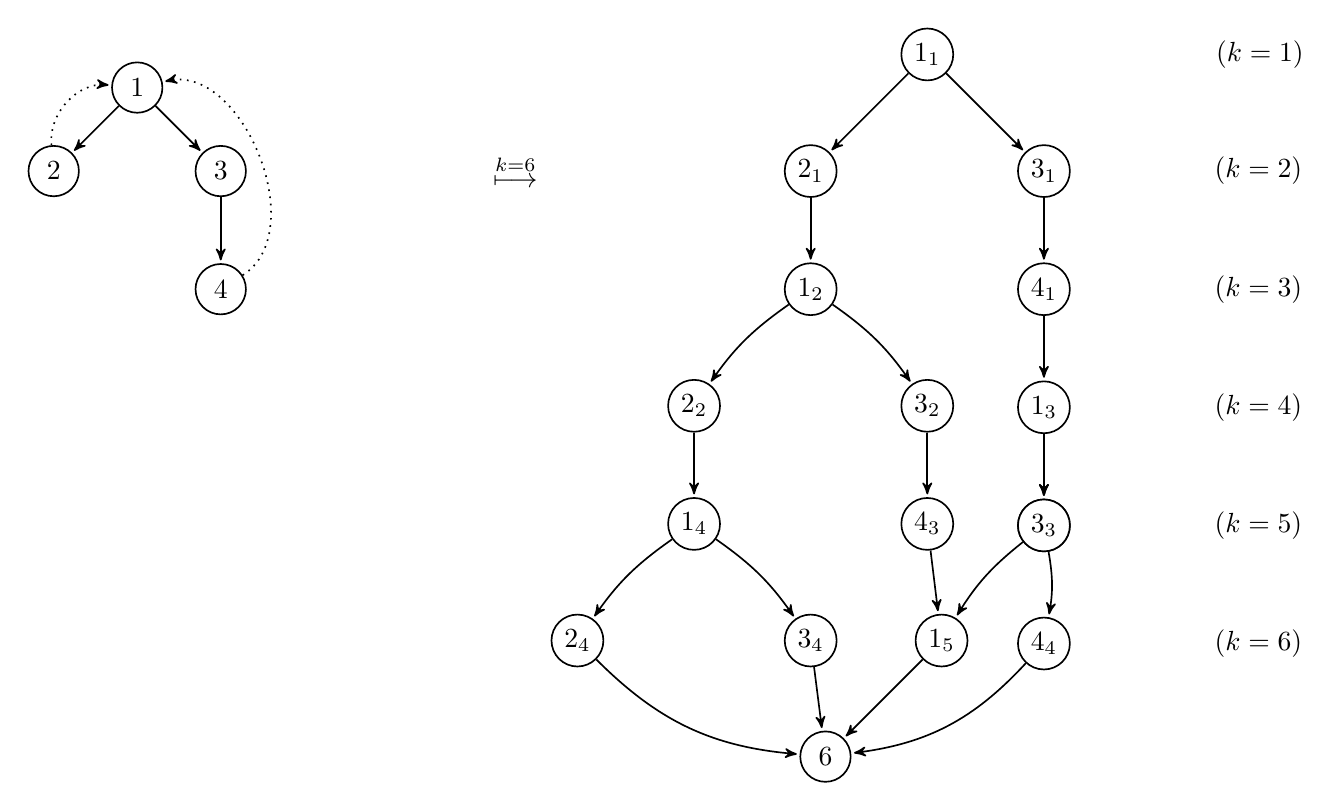
\begin{tikzpicture}[->,>=stealth',shorten >=1pt,auto,node distance=1.5cm,semithick]
\node[c] (1) [] {$1$};
\node[c] (2) [below left of=1] {$2$};
\node[c] (3) [below right of=1] {$3$};
\node[c] (4) [below of=3] {$4$};
\path[->]
(1) edge [] node {} (2)
(2) edge [bend left=50,dotted] node {} (1)
(1) edge [] node {} (3)
(3) edge [] node {} (4)
(4) edge [bend right=80,dotted] node {} (1)
;
\node[draw=none] (impl) [right=3cm of 3] {$\overset{k = 6}{\longmapsto}$};
;
\node[c] (21) [right=3cm of impl] {$2_1$};
\node[c] (11) [above right=1cm and 1cm of 21]{$1_1$};
\node[c] (31) [below right=1cm and 1cm of 11] {$3_1$};
\node[c] (41) [below of=31] {$4_1$};
\node[c] (12) [below of=21] {$1_2$};
\node[c] (22) [below left=1cm and 1cm of 12] {$2_2$};
\node[c] (32) [below right=1cm and 1cm of 12] {$3_2$};
\node[c] (13) [below of=41] {$1_3$};
\node[c] (14) [below of=22] {$1_4$};
\node[c] (43) [below of=32] {$4_3$};
\node[c] (23) [below of=13] {$2_3$};
\node[c] (33) [below of=13] {$3_3$};
\node[c] (24) [below left=1cm and 1cm of 14] {$2_4$};
\node[c] (34) [below right=1cm and 1cm of 14] {$3_4$};
\node[c] (15) [below right=1cm and -0.3cm of 43] {$1_5$};
\node[c] (44) [below of=33] {$4_4$};
\node[c] (6) [below left=1cm and 1cm of 15] {$6$};
\node[] (11k) [right=3.2cm of 11] {$(k = 1)$};
\node[] (31k) [right=1.7cm of 31] {$(k = 2)$};
\node[] (41k) [right=1.7cm of 41] {$(k = 3)$};
\node[] (13k) [right=1.7cm of 13] {$(k = 4)$};
\node[] (33k) [right=1.7cm of 33] {$(k = 5)$};
\node[] (44k) [right=1.7cm of 44] {$(k = 6)$};
\path[->]
(11) edge [] node {} (21)
(11) edge [] node {} (31)
(31) edge [] node {} (41)
(21) edge [] node {} (12)
(12) edge [bend right=10] node {} (22)
(12) edge [bend left=10] node {} (32)
(41) edge [] node {} (13)
(22) edge [] node {} (14)
(32) edge [] node {} (43)
(13) edge [] node {} (23)
(13) edge [] node {} (33)
(14) edge [bend right=10] node {} (24)
(14) edge [bend left=10] node {} (34)
(43) edge [] node {} (15)
(33) edge [bend right=10] node {} (15)
(33) edge [bend left=10] node {} (44)
(24) edge [bend right=20] node {} (6)
(34) edge [] node {} (6)
(15) edge [] node {} (6)
(44) edge [bend left=20] node {} (6)
;
\end{tikzpicture}
\caption{Example of the flow graph from Figure~\ref{fig:merged-loop}, unwinded up to the bound $k = 6$} \label{fig:merged-loop}
\end{figure}

\end{document}

" 
%pdflatex -output-directory=out "
\documentclass[12pt,a4paper,oneside,pdftex]{report}


\usepackage{subcaption}
\usepackage{graphicx}
\usepackage{amsmath}

\usepackage{tikz}
\usetikzlibrary{positioning}
\usetikzlibrary{calc}
\usetikzlibrary{arrows}
\usetikzlibrary{decorations.pathmorphing,decorations.markings}
\usetikzlibrary{shapes}
\usetikzlibrary{patterns}
\usetikzlibrary{automata}

\tikzset{
c/.style={
  circle,
  inner sep=0pt,
  text width=6mm,
  align=center,
  draw=black,
  fill=white
  }
}


\begin{document}

Hello

\section{Kakashka}
blub

%pdflatex -output-directory=out "\def\IsAalto{yes} \input{test.tex}" 
%pdflatex -output-directory=out "\input{test.tex}" 
\ifdefined\IsAalto
  def
\else
  non-def
\fi

\begin{figure}
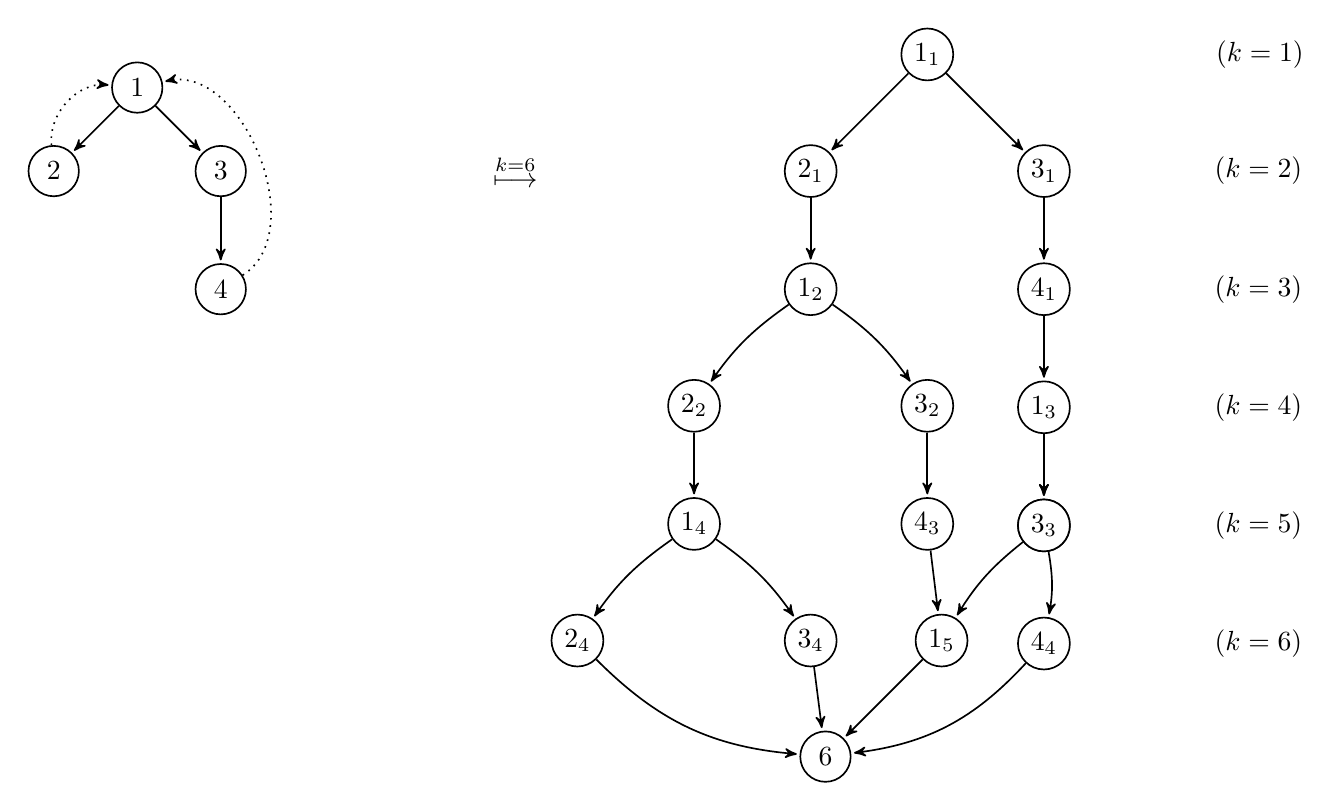
\begin{tikzpicture}[->,>=stealth',shorten >=1pt,auto,node distance=1.5cm,semithick]
\node[c] (1) [] {$1$};
\node[c] (2) [below left of=1] {$2$};
\node[c] (3) [below right of=1] {$3$};
\node[c] (4) [below of=3] {$4$};
\path[->]
(1) edge [] node {} (2)
(2) edge [bend left=50,dotted] node {} (1)
(1) edge [] node {} (3)
(3) edge [] node {} (4)
(4) edge [bend right=80,dotted] node {} (1)
;
\node[draw=none] (impl) [right=3cm of 3] {$\overset{k = 6}{\longmapsto}$};
;
\node[c] (21) [right=3cm of impl] {$2_1$};
\node[c] (11) [above right=1cm and 1cm of 21]{$1_1$};
\node[c] (31) [below right=1cm and 1cm of 11] {$3_1$};
\node[c] (41) [below of=31] {$4_1$};
\node[c] (12) [below of=21] {$1_2$};
\node[c] (22) [below left=1cm and 1cm of 12] {$2_2$};
\node[c] (32) [below right=1cm and 1cm of 12] {$3_2$};
\node[c] (13) [below of=41] {$1_3$};
\node[c] (14) [below of=22] {$1_4$};
\node[c] (43) [below of=32] {$4_3$};
\node[c] (23) [below of=13] {$2_3$};
\node[c] (33) [below of=13] {$3_3$};
\node[c] (24) [below left=1cm and 1cm of 14] {$2_4$};
\node[c] (34) [below right=1cm and 1cm of 14] {$3_4$};
\node[c] (15) [below right=1cm and -0.3cm of 43] {$1_5$};
\node[c] (44) [below of=33] {$4_4$};
\node[c] (6) [below left=1cm and 1cm of 15] {$6$};
\node[] (11k) [right=3.2cm of 11] {$(k = 1)$};
\node[] (31k) [right=1.7cm of 31] {$(k = 2)$};
\node[] (41k) [right=1.7cm of 41] {$(k = 3)$};
\node[] (13k) [right=1.7cm of 13] {$(k = 4)$};
\node[] (33k) [right=1.7cm of 33] {$(k = 5)$};
\node[] (44k) [right=1.7cm of 44] {$(k = 6)$};
\path[->]
(11) edge [] node {} (21)
(11) edge [] node {} (31)
(31) edge [] node {} (41)
(21) edge [] node {} (12)
(12) edge [bend right=10] node {} (22)
(12) edge [bend left=10] node {} (32)
(41) edge [] node {} (13)
(22) edge [] node {} (14)
(32) edge [] node {} (43)
(13) edge [] node {} (23)
(13) edge [] node {} (33)
(14) edge [bend right=10] node {} (24)
(14) edge [bend left=10] node {} (34)
(43) edge [] node {} (15)
(33) edge [bend right=10] node {} (15)
(33) edge [bend left=10] node {} (44)
(24) edge [bend right=20] node {} (6)
(34) edge [] node {} (6)
(15) edge [] node {} (6)
(44) edge [bend left=20] node {} (6)
;
\end{tikzpicture}
\caption{Example of the flow graph from Figure~\ref{fig:merged-loop}, unwinded up to the bound $k = 6$} \label{fig:merged-loop}
\end{figure}

\end{document}

" 
\ifdefined\IsAalto
  def
\else
  non-def
\fi

\begin{figure}
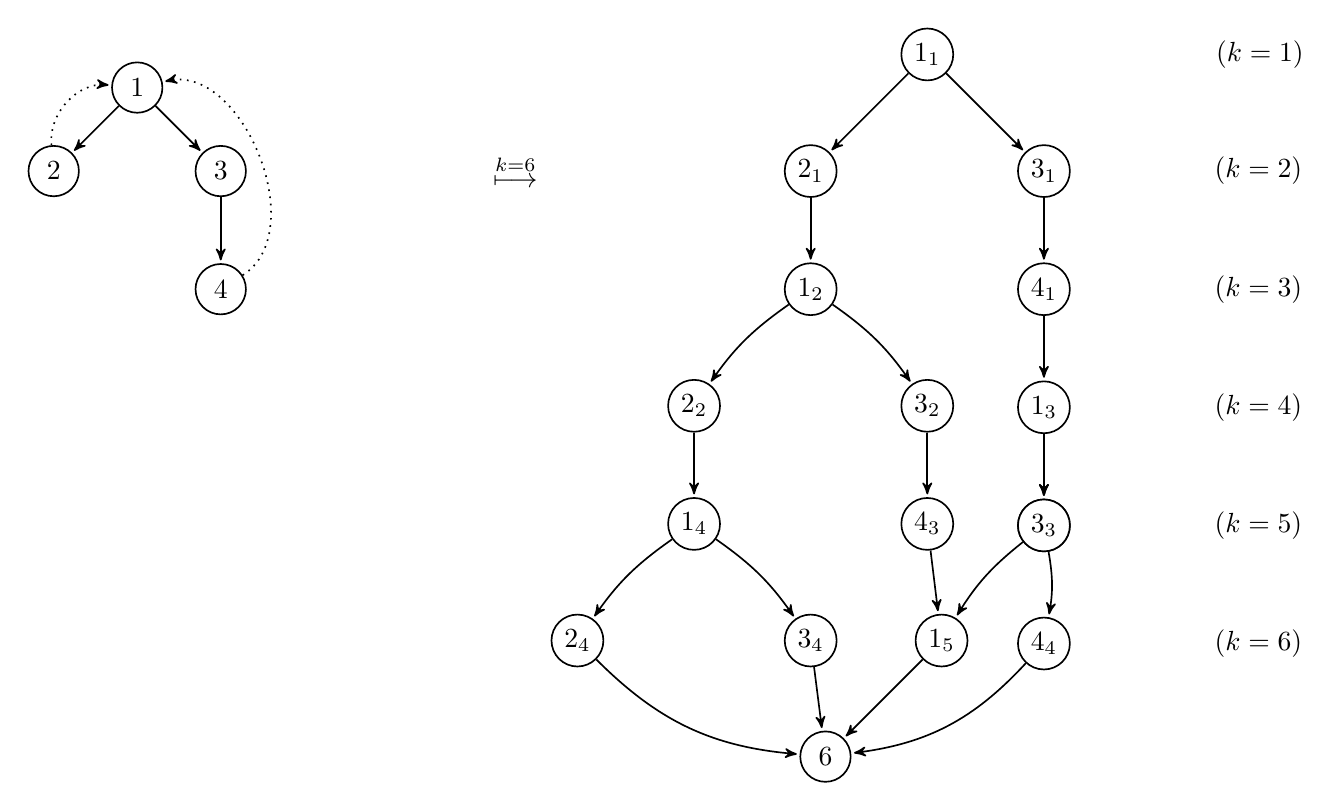
\begin{tikzpicture}[->,>=stealth',shorten >=1pt,auto,node distance=1.5cm,semithick]
\node[c] (1) [] {$1$};
\node[c] (2) [below left of=1] {$2$};
\node[c] (3) [below right of=1] {$3$};
\node[c] (4) [below of=3] {$4$};
\path[->]
(1) edge [] node {} (2)
(2) edge [bend left=50,dotted] node {} (1)
(1) edge [] node {} (3)
(3) edge [] node {} (4)
(4) edge [bend right=80,dotted] node {} (1)
;
\node[draw=none] (impl) [right=3cm of 3] {$\overset{k = 6}{\longmapsto}$};
;
\node[c] (21) [right=3cm of impl] {$2_1$};
\node[c] (11) [above right=1cm and 1cm of 21]{$1_1$};
\node[c] (31) [below right=1cm and 1cm of 11] {$3_1$};
\node[c] (41) [below of=31] {$4_1$};
\node[c] (12) [below of=21] {$1_2$};
\node[c] (22) [below left=1cm and 1cm of 12] {$2_2$};
\node[c] (32) [below right=1cm and 1cm of 12] {$3_2$};
\node[c] (13) [below of=41] {$1_3$};
\node[c] (14) [below of=22] {$1_4$};
\node[c] (43) [below of=32] {$4_3$};
\node[c] (23) [below of=13] {$2_3$};
\node[c] (33) [below of=13] {$3_3$};
\node[c] (24) [below left=1cm and 1cm of 14] {$2_4$};
\node[c] (34) [below right=1cm and 1cm of 14] {$3_4$};
\node[c] (15) [below right=1cm and -0.3cm of 43] {$1_5$};
\node[c] (44) [below of=33] {$4_4$};
\node[c] (6) [below left=1cm and 1cm of 15] {$6$};
\node[] (11k) [right=3.2cm of 11] {$(k = 1)$};
\node[] (31k) [right=1.7cm of 31] {$(k = 2)$};
\node[] (41k) [right=1.7cm of 41] {$(k = 3)$};
\node[] (13k) [right=1.7cm of 13] {$(k = 4)$};
\node[] (33k) [right=1.7cm of 33] {$(k = 5)$};
\node[] (44k) [right=1.7cm of 44] {$(k = 6)$};
\path[->]
(11) edge [] node {} (21)
(11) edge [] node {} (31)
(31) edge [] node {} (41)
(21) edge [] node {} (12)
(12) edge [bend right=10] node {} (22)
(12) edge [bend left=10] node {} (32)
(41) edge [] node {} (13)
(22) edge [] node {} (14)
(32) edge [] node {} (43)
(13) edge [] node {} (23)
(13) edge [] node {} (33)
(14) edge [bend right=10] node {} (24)
(14) edge [bend left=10] node {} (34)
(43) edge [] node {} (15)
(33) edge [bend right=10] node {} (15)
(33) edge [bend left=10] node {} (44)
(24) edge [bend right=20] node {} (6)
(34) edge [] node {} (6)
(15) edge [] node {} (6)
(44) edge [bend left=20] node {} (6)
;
\end{tikzpicture}
\caption{Example of the flow graph from Figure~\ref{fig:merged-loop}, unwinded up to the bound $k = 6$} \label{fig:merged-loop}
\end{figure}

\end{document}

" 
\ifdefined\IsAalto
  def
\else
  non-def
\fi

\begin{figure}
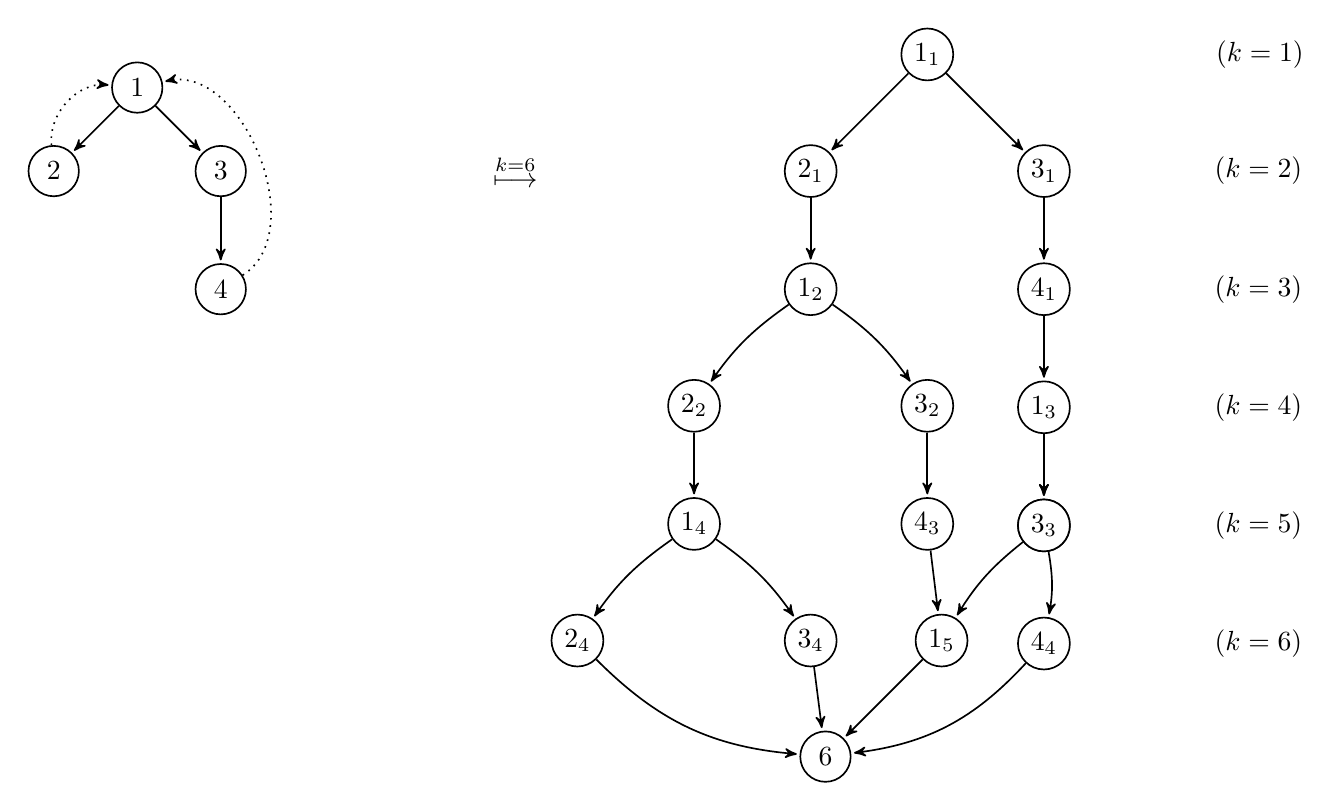
\begin{tikzpicture}[->,>=stealth',shorten >=1pt,auto,node distance=1.5cm,semithick]
\node[c] (1) [] {$1$};
\node[c] (2) [below left of=1] {$2$};
\node[c] (3) [below right of=1] {$3$};
\node[c] (4) [below of=3] {$4$};
\path[->]
(1) edge [] node {} (2)
(2) edge [bend left=50,dotted] node {} (1)
(1) edge [] node {} (3)
(3) edge [] node {} (4)
(4) edge [bend right=80,dotted] node {} (1)
;
\node[draw=none] (impl) [right=3cm of 3] {$\overset{k = 6}{\longmapsto}$};
;
\node[c] (21) [right=3cm of impl] {$2_1$};
\node[c] (11) [above right=1cm and 1cm of 21]{$1_1$};
\node[c] (31) [below right=1cm and 1cm of 11] {$3_1$};
\node[c] (41) [below of=31] {$4_1$};
\node[c] (12) [below of=21] {$1_2$};
\node[c] (22) [below left=1cm and 1cm of 12] {$2_2$};
\node[c] (32) [below right=1cm and 1cm of 12] {$3_2$};
\node[c] (13) [below of=41] {$1_3$};
\node[c] (14) [below of=22] {$1_4$};
\node[c] (43) [below of=32] {$4_3$};
\node[c] (23) [below of=13] {$2_3$};
\node[c] (33) [below of=13] {$3_3$};
\node[c] (24) [below left=1cm and 1cm of 14] {$2_4$};
\node[c] (34) [below right=1cm and 1cm of 14] {$3_4$};
\node[c] (15) [below right=1cm and -0.3cm of 43] {$1_5$};
\node[c] (44) [below of=33] {$4_4$};
\node[c] (6) [below left=1cm and 1cm of 15] {$6$};
\node[] (11k) [right=3.2cm of 11] {$(k = 1)$};
\node[] (31k) [right=1.7cm of 31] {$(k = 2)$};
\node[] (41k) [right=1.7cm of 41] {$(k = 3)$};
\node[] (13k) [right=1.7cm of 13] {$(k = 4)$};
\node[] (33k) [right=1.7cm of 33] {$(k = 5)$};
\node[] (44k) [right=1.7cm of 44] {$(k = 6)$};
\path[->]
(11) edge [] node {} (21)
(11) edge [] node {} (31)
(31) edge [] node {} (41)
(21) edge [] node {} (12)
(12) edge [bend right=10] node {} (22)
(12) edge [bend left=10] node {} (32)
(41) edge [] node {} (13)
(22) edge [] node {} (14)
(32) edge [] node {} (43)
(13) edge [] node {} (23)
(13) edge [] node {} (33)
(14) edge [bend right=10] node {} (24)
(14) edge [bend left=10] node {} (34)
(43) edge [] node {} (15)
(33) edge [bend right=10] node {} (15)
(33) edge [bend left=10] node {} (44)
(24) edge [bend right=20] node {} (6)
(34) edge [] node {} (6)
(15) edge [] node {} (6)
(44) edge [bend left=20] node {} (6)
;
\end{tikzpicture}
\caption{Example of the flow graph from Figure~\ref{fig:merged-loop}, unwinded up to the bound $k = 6$} \label{fig:merged-loop}
\end{figure}

\end{document}

" 
%pdflatex -output-directory=out "
\documentclass[12pt,a4paper,oneside,pdftex]{report}


\usepackage{subcaption}
\usepackage{graphicx}
\usepackage{amsmath}

\usepackage{tikz}
\usetikzlibrary{positioning}
\usetikzlibrary{calc}
\usetikzlibrary{arrows}
\usetikzlibrary{decorations.pathmorphing,decorations.markings}
\usetikzlibrary{shapes}
\usetikzlibrary{patterns}
\usetikzlibrary{automata}

\tikzset{
c/.style={
  circle,
  inner sep=0pt,
  text width=6mm,
  align=center,
  draw=black,
  fill=white
  }
}


\begin{document}

Hello

\section{Kakashka}
blub

%pdflatex -output-directory=out "\def\IsAalto{yes} 
\documentclass[12pt,a4paper,oneside,pdftex]{report}


\usepackage{subcaption}
\usepackage{graphicx}
\usepackage{amsmath}

\usepackage{tikz}
\usetikzlibrary{positioning}
\usetikzlibrary{calc}
\usetikzlibrary{arrows}
\usetikzlibrary{decorations.pathmorphing,decorations.markings}
\usetikzlibrary{shapes}
\usetikzlibrary{patterns}
\usetikzlibrary{automata}

\tikzset{
c/.style={
  circle,
  inner sep=0pt,
  text width=6mm,
  align=center,
  draw=black,
  fill=white
  }
}


\begin{document}

Hello

\section{Kakashka}
blub

%pdflatex -output-directory=out "\def\IsAalto{yes} 
\documentclass[12pt,a4paper,oneside,pdftex]{report}


\usepackage{subcaption}
\usepackage{graphicx}
\usepackage{amsmath}

\usepackage{tikz}
\usetikzlibrary{positioning}
\usetikzlibrary{calc}
\usetikzlibrary{arrows}
\usetikzlibrary{decorations.pathmorphing,decorations.markings}
\usetikzlibrary{shapes}
\usetikzlibrary{patterns}
\usetikzlibrary{automata}

\tikzset{
c/.style={
  circle,
  inner sep=0pt,
  text width=6mm,
  align=center,
  draw=black,
  fill=white
  }
}


\begin{document}

Hello

\section{Kakashka}
blub

%pdflatex -output-directory=out "\def\IsAalto{yes} \input{test.tex}" 
%pdflatex -output-directory=out "\input{test.tex}" 
\ifdefined\IsAalto
  def
\else
  non-def
\fi

\begin{figure}
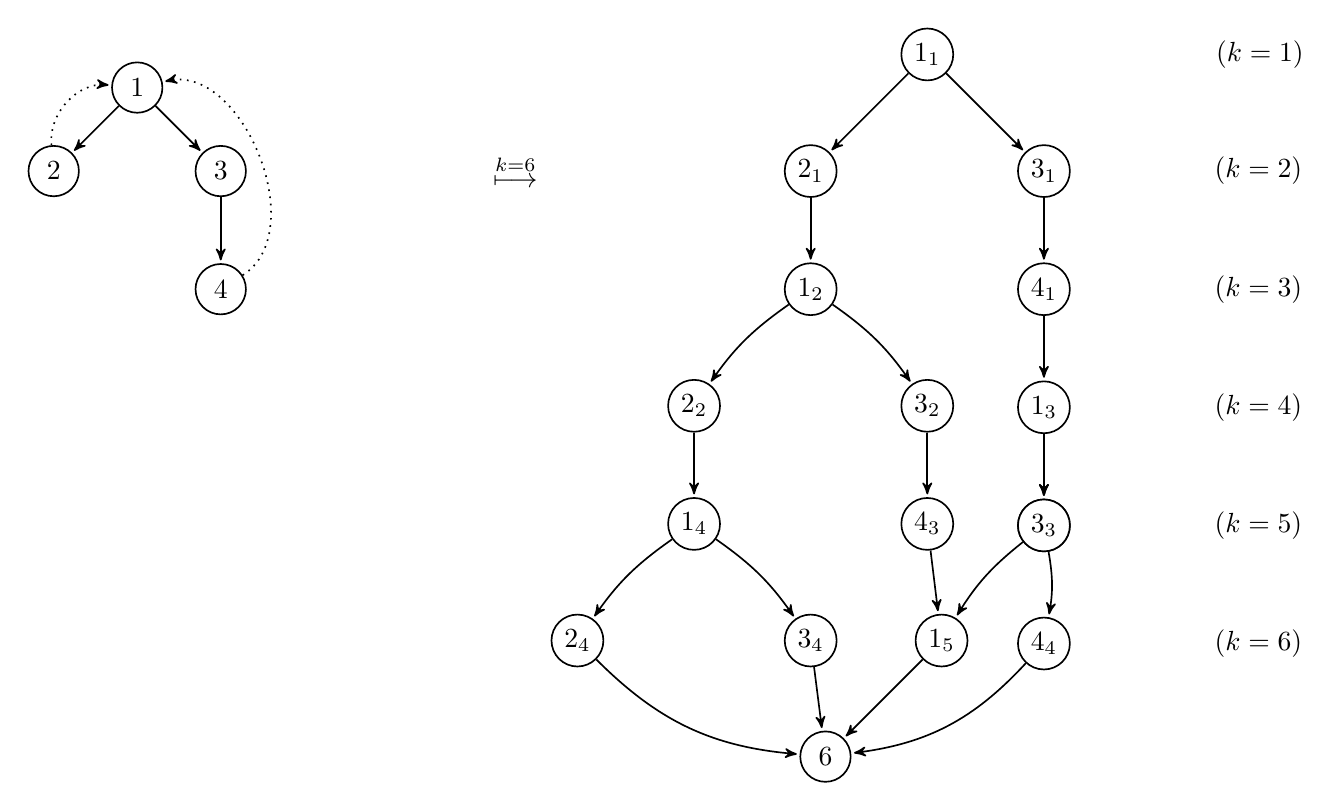
\begin{tikzpicture}[->,>=stealth',shorten >=1pt,auto,node distance=1.5cm,semithick]
\node[c] (1) [] {$1$};
\node[c] (2) [below left of=1] {$2$};
\node[c] (3) [below right of=1] {$3$};
\node[c] (4) [below of=3] {$4$};
\path[->]
(1) edge [] node {} (2)
(2) edge [bend left=50,dotted] node {} (1)
(1) edge [] node {} (3)
(3) edge [] node {} (4)
(4) edge [bend right=80,dotted] node {} (1)
;
\node[draw=none] (impl) [right=3cm of 3] {$\overset{k = 6}{\longmapsto}$};
;
\node[c] (21) [right=3cm of impl] {$2_1$};
\node[c] (11) [above right=1cm and 1cm of 21]{$1_1$};
\node[c] (31) [below right=1cm and 1cm of 11] {$3_1$};
\node[c] (41) [below of=31] {$4_1$};
\node[c] (12) [below of=21] {$1_2$};
\node[c] (22) [below left=1cm and 1cm of 12] {$2_2$};
\node[c] (32) [below right=1cm and 1cm of 12] {$3_2$};
\node[c] (13) [below of=41] {$1_3$};
\node[c] (14) [below of=22] {$1_4$};
\node[c] (43) [below of=32] {$4_3$};
\node[c] (23) [below of=13] {$2_3$};
\node[c] (33) [below of=13] {$3_3$};
\node[c] (24) [below left=1cm and 1cm of 14] {$2_4$};
\node[c] (34) [below right=1cm and 1cm of 14] {$3_4$};
\node[c] (15) [below right=1cm and -0.3cm of 43] {$1_5$};
\node[c] (44) [below of=33] {$4_4$};
\node[c] (6) [below left=1cm and 1cm of 15] {$6$};
\node[] (11k) [right=3.2cm of 11] {$(k = 1)$};
\node[] (31k) [right=1.7cm of 31] {$(k = 2)$};
\node[] (41k) [right=1.7cm of 41] {$(k = 3)$};
\node[] (13k) [right=1.7cm of 13] {$(k = 4)$};
\node[] (33k) [right=1.7cm of 33] {$(k = 5)$};
\node[] (44k) [right=1.7cm of 44] {$(k = 6)$};
\path[->]
(11) edge [] node {} (21)
(11) edge [] node {} (31)
(31) edge [] node {} (41)
(21) edge [] node {} (12)
(12) edge [bend right=10] node {} (22)
(12) edge [bend left=10] node {} (32)
(41) edge [] node {} (13)
(22) edge [] node {} (14)
(32) edge [] node {} (43)
(13) edge [] node {} (23)
(13) edge [] node {} (33)
(14) edge [bend right=10] node {} (24)
(14) edge [bend left=10] node {} (34)
(43) edge [] node {} (15)
(33) edge [bend right=10] node {} (15)
(33) edge [bend left=10] node {} (44)
(24) edge [bend right=20] node {} (6)
(34) edge [] node {} (6)
(15) edge [] node {} (6)
(44) edge [bend left=20] node {} (6)
;
\end{tikzpicture}
\caption{Example of the flow graph from Figure~\ref{fig:merged-loop}, unwinded up to the bound $k = 6$} \label{fig:merged-loop}
\end{figure}

\end{document}

" 
%pdflatex -output-directory=out "
\documentclass[12pt,a4paper,oneside,pdftex]{report}


\usepackage{subcaption}
\usepackage{graphicx}
\usepackage{amsmath}

\usepackage{tikz}
\usetikzlibrary{positioning}
\usetikzlibrary{calc}
\usetikzlibrary{arrows}
\usetikzlibrary{decorations.pathmorphing,decorations.markings}
\usetikzlibrary{shapes}
\usetikzlibrary{patterns}
\usetikzlibrary{automata}

\tikzset{
c/.style={
  circle,
  inner sep=0pt,
  text width=6mm,
  align=center,
  draw=black,
  fill=white
  }
}


\begin{document}

Hello

\section{Kakashka}
blub

%pdflatex -output-directory=out "\def\IsAalto{yes} \input{test.tex}" 
%pdflatex -output-directory=out "\input{test.tex}" 
\ifdefined\IsAalto
  def
\else
  non-def
\fi

\begin{figure}
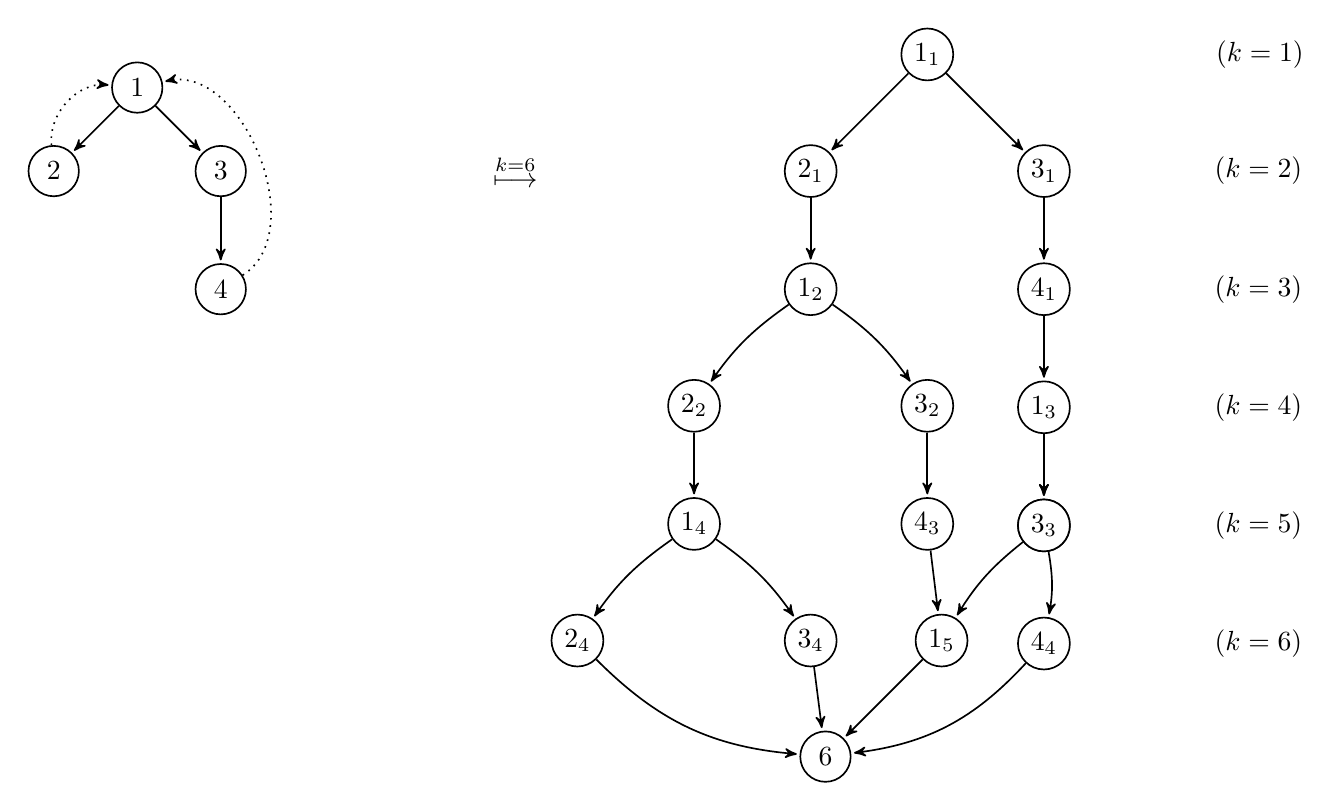
\begin{tikzpicture}[->,>=stealth',shorten >=1pt,auto,node distance=1.5cm,semithick]
\node[c] (1) [] {$1$};
\node[c] (2) [below left of=1] {$2$};
\node[c] (3) [below right of=1] {$3$};
\node[c] (4) [below of=3] {$4$};
\path[->]
(1) edge [] node {} (2)
(2) edge [bend left=50,dotted] node {} (1)
(1) edge [] node {} (3)
(3) edge [] node {} (4)
(4) edge [bend right=80,dotted] node {} (1)
;
\node[draw=none] (impl) [right=3cm of 3] {$\overset{k = 6}{\longmapsto}$};
;
\node[c] (21) [right=3cm of impl] {$2_1$};
\node[c] (11) [above right=1cm and 1cm of 21]{$1_1$};
\node[c] (31) [below right=1cm and 1cm of 11] {$3_1$};
\node[c] (41) [below of=31] {$4_1$};
\node[c] (12) [below of=21] {$1_2$};
\node[c] (22) [below left=1cm and 1cm of 12] {$2_2$};
\node[c] (32) [below right=1cm and 1cm of 12] {$3_2$};
\node[c] (13) [below of=41] {$1_3$};
\node[c] (14) [below of=22] {$1_4$};
\node[c] (43) [below of=32] {$4_3$};
\node[c] (23) [below of=13] {$2_3$};
\node[c] (33) [below of=13] {$3_3$};
\node[c] (24) [below left=1cm and 1cm of 14] {$2_4$};
\node[c] (34) [below right=1cm and 1cm of 14] {$3_4$};
\node[c] (15) [below right=1cm and -0.3cm of 43] {$1_5$};
\node[c] (44) [below of=33] {$4_4$};
\node[c] (6) [below left=1cm and 1cm of 15] {$6$};
\node[] (11k) [right=3.2cm of 11] {$(k = 1)$};
\node[] (31k) [right=1.7cm of 31] {$(k = 2)$};
\node[] (41k) [right=1.7cm of 41] {$(k = 3)$};
\node[] (13k) [right=1.7cm of 13] {$(k = 4)$};
\node[] (33k) [right=1.7cm of 33] {$(k = 5)$};
\node[] (44k) [right=1.7cm of 44] {$(k = 6)$};
\path[->]
(11) edge [] node {} (21)
(11) edge [] node {} (31)
(31) edge [] node {} (41)
(21) edge [] node {} (12)
(12) edge [bend right=10] node {} (22)
(12) edge [bend left=10] node {} (32)
(41) edge [] node {} (13)
(22) edge [] node {} (14)
(32) edge [] node {} (43)
(13) edge [] node {} (23)
(13) edge [] node {} (33)
(14) edge [bend right=10] node {} (24)
(14) edge [bend left=10] node {} (34)
(43) edge [] node {} (15)
(33) edge [bend right=10] node {} (15)
(33) edge [bend left=10] node {} (44)
(24) edge [bend right=20] node {} (6)
(34) edge [] node {} (6)
(15) edge [] node {} (6)
(44) edge [bend left=20] node {} (6)
;
\end{tikzpicture}
\caption{Example of the flow graph from Figure~\ref{fig:merged-loop}, unwinded up to the bound $k = 6$} \label{fig:merged-loop}
\end{figure}

\end{document}

" 
\ifdefined\IsAalto
  def
\else
  non-def
\fi

\begin{figure}
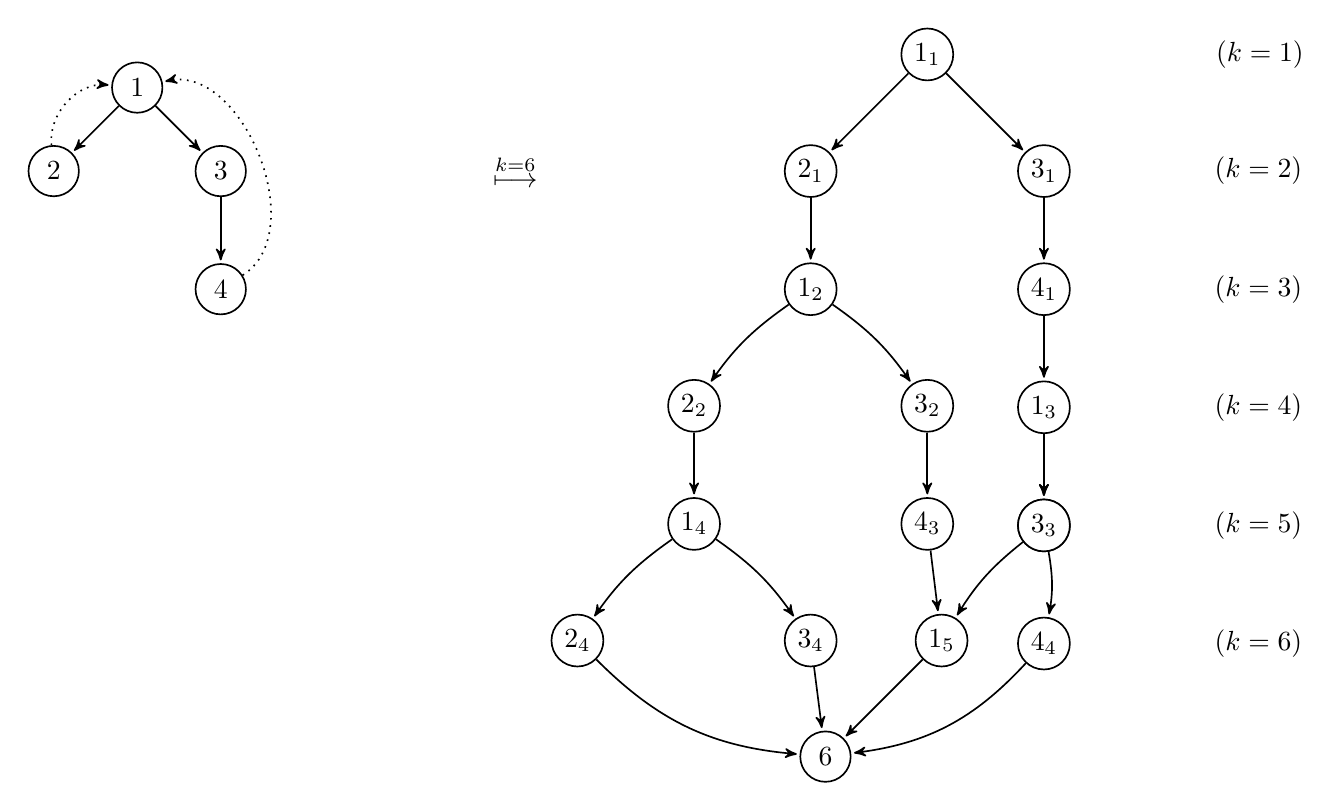
\begin{tikzpicture}[->,>=stealth',shorten >=1pt,auto,node distance=1.5cm,semithick]
\node[c] (1) [] {$1$};
\node[c] (2) [below left of=1] {$2$};
\node[c] (3) [below right of=1] {$3$};
\node[c] (4) [below of=3] {$4$};
\path[->]
(1) edge [] node {} (2)
(2) edge [bend left=50,dotted] node {} (1)
(1) edge [] node {} (3)
(3) edge [] node {} (4)
(4) edge [bend right=80,dotted] node {} (1)
;
\node[draw=none] (impl) [right=3cm of 3] {$\overset{k = 6}{\longmapsto}$};
;
\node[c] (21) [right=3cm of impl] {$2_1$};
\node[c] (11) [above right=1cm and 1cm of 21]{$1_1$};
\node[c] (31) [below right=1cm and 1cm of 11] {$3_1$};
\node[c] (41) [below of=31] {$4_1$};
\node[c] (12) [below of=21] {$1_2$};
\node[c] (22) [below left=1cm and 1cm of 12] {$2_2$};
\node[c] (32) [below right=1cm and 1cm of 12] {$3_2$};
\node[c] (13) [below of=41] {$1_3$};
\node[c] (14) [below of=22] {$1_4$};
\node[c] (43) [below of=32] {$4_3$};
\node[c] (23) [below of=13] {$2_3$};
\node[c] (33) [below of=13] {$3_3$};
\node[c] (24) [below left=1cm and 1cm of 14] {$2_4$};
\node[c] (34) [below right=1cm and 1cm of 14] {$3_4$};
\node[c] (15) [below right=1cm and -0.3cm of 43] {$1_5$};
\node[c] (44) [below of=33] {$4_4$};
\node[c] (6) [below left=1cm and 1cm of 15] {$6$};
\node[] (11k) [right=3.2cm of 11] {$(k = 1)$};
\node[] (31k) [right=1.7cm of 31] {$(k = 2)$};
\node[] (41k) [right=1.7cm of 41] {$(k = 3)$};
\node[] (13k) [right=1.7cm of 13] {$(k = 4)$};
\node[] (33k) [right=1.7cm of 33] {$(k = 5)$};
\node[] (44k) [right=1.7cm of 44] {$(k = 6)$};
\path[->]
(11) edge [] node {} (21)
(11) edge [] node {} (31)
(31) edge [] node {} (41)
(21) edge [] node {} (12)
(12) edge [bend right=10] node {} (22)
(12) edge [bend left=10] node {} (32)
(41) edge [] node {} (13)
(22) edge [] node {} (14)
(32) edge [] node {} (43)
(13) edge [] node {} (23)
(13) edge [] node {} (33)
(14) edge [bend right=10] node {} (24)
(14) edge [bend left=10] node {} (34)
(43) edge [] node {} (15)
(33) edge [bend right=10] node {} (15)
(33) edge [bend left=10] node {} (44)
(24) edge [bend right=20] node {} (6)
(34) edge [] node {} (6)
(15) edge [] node {} (6)
(44) edge [bend left=20] node {} (6)
;
\end{tikzpicture}
\caption{Example of the flow graph from Figure~\ref{fig:merged-loop}, unwinded up to the bound $k = 6$} \label{fig:merged-loop}
\end{figure}

\end{document}

" 
%pdflatex -output-directory=out "
\documentclass[12pt,a4paper,oneside,pdftex]{report}


\usepackage{subcaption}
\usepackage{graphicx}
\usepackage{amsmath}

\usepackage{tikz}
\usetikzlibrary{positioning}
\usetikzlibrary{calc}
\usetikzlibrary{arrows}
\usetikzlibrary{decorations.pathmorphing,decorations.markings}
\usetikzlibrary{shapes}
\usetikzlibrary{patterns}
\usetikzlibrary{automata}

\tikzset{
c/.style={
  circle,
  inner sep=0pt,
  text width=6mm,
  align=center,
  draw=black,
  fill=white
  }
}


\begin{document}

Hello

\section{Kakashka}
blub

%pdflatex -output-directory=out "\def\IsAalto{yes} 
\documentclass[12pt,a4paper,oneside,pdftex]{report}


\usepackage{subcaption}
\usepackage{graphicx}
\usepackage{amsmath}

\usepackage{tikz}
\usetikzlibrary{positioning}
\usetikzlibrary{calc}
\usetikzlibrary{arrows}
\usetikzlibrary{decorations.pathmorphing,decorations.markings}
\usetikzlibrary{shapes}
\usetikzlibrary{patterns}
\usetikzlibrary{automata}

\tikzset{
c/.style={
  circle,
  inner sep=0pt,
  text width=6mm,
  align=center,
  draw=black,
  fill=white
  }
}


\begin{document}

Hello

\section{Kakashka}
blub

%pdflatex -output-directory=out "\def\IsAalto{yes} \input{test.tex}" 
%pdflatex -output-directory=out "\input{test.tex}" 
\ifdefined\IsAalto
  def
\else
  non-def
\fi

\begin{figure}
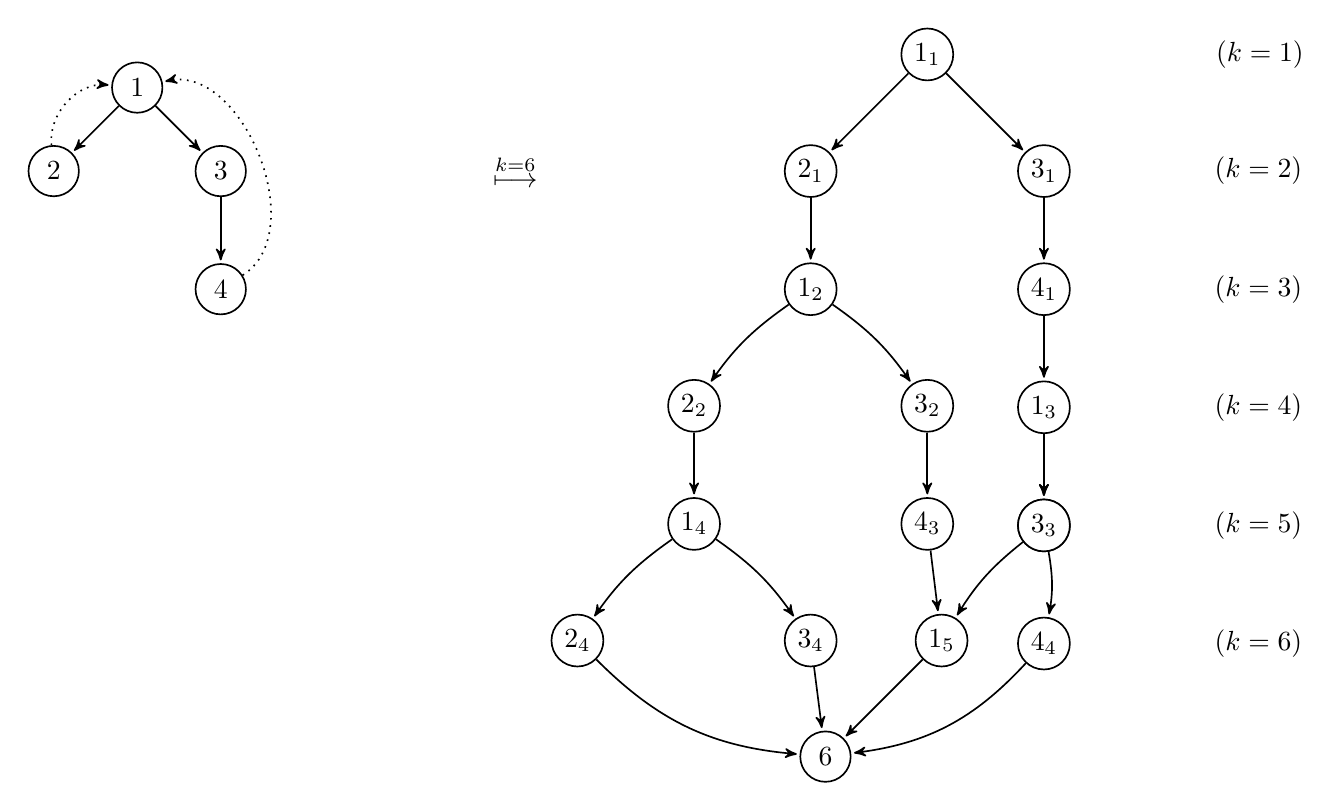
\begin{tikzpicture}[->,>=stealth',shorten >=1pt,auto,node distance=1.5cm,semithick]
\node[c] (1) [] {$1$};
\node[c] (2) [below left of=1] {$2$};
\node[c] (3) [below right of=1] {$3$};
\node[c] (4) [below of=3] {$4$};
\path[->]
(1) edge [] node {} (2)
(2) edge [bend left=50,dotted] node {} (1)
(1) edge [] node {} (3)
(3) edge [] node {} (4)
(4) edge [bend right=80,dotted] node {} (1)
;
\node[draw=none] (impl) [right=3cm of 3] {$\overset{k = 6}{\longmapsto}$};
;
\node[c] (21) [right=3cm of impl] {$2_1$};
\node[c] (11) [above right=1cm and 1cm of 21]{$1_1$};
\node[c] (31) [below right=1cm and 1cm of 11] {$3_1$};
\node[c] (41) [below of=31] {$4_1$};
\node[c] (12) [below of=21] {$1_2$};
\node[c] (22) [below left=1cm and 1cm of 12] {$2_2$};
\node[c] (32) [below right=1cm and 1cm of 12] {$3_2$};
\node[c] (13) [below of=41] {$1_3$};
\node[c] (14) [below of=22] {$1_4$};
\node[c] (43) [below of=32] {$4_3$};
\node[c] (23) [below of=13] {$2_3$};
\node[c] (33) [below of=13] {$3_3$};
\node[c] (24) [below left=1cm and 1cm of 14] {$2_4$};
\node[c] (34) [below right=1cm and 1cm of 14] {$3_4$};
\node[c] (15) [below right=1cm and -0.3cm of 43] {$1_5$};
\node[c] (44) [below of=33] {$4_4$};
\node[c] (6) [below left=1cm and 1cm of 15] {$6$};
\node[] (11k) [right=3.2cm of 11] {$(k = 1)$};
\node[] (31k) [right=1.7cm of 31] {$(k = 2)$};
\node[] (41k) [right=1.7cm of 41] {$(k = 3)$};
\node[] (13k) [right=1.7cm of 13] {$(k = 4)$};
\node[] (33k) [right=1.7cm of 33] {$(k = 5)$};
\node[] (44k) [right=1.7cm of 44] {$(k = 6)$};
\path[->]
(11) edge [] node {} (21)
(11) edge [] node {} (31)
(31) edge [] node {} (41)
(21) edge [] node {} (12)
(12) edge [bend right=10] node {} (22)
(12) edge [bend left=10] node {} (32)
(41) edge [] node {} (13)
(22) edge [] node {} (14)
(32) edge [] node {} (43)
(13) edge [] node {} (23)
(13) edge [] node {} (33)
(14) edge [bend right=10] node {} (24)
(14) edge [bend left=10] node {} (34)
(43) edge [] node {} (15)
(33) edge [bend right=10] node {} (15)
(33) edge [bend left=10] node {} (44)
(24) edge [bend right=20] node {} (6)
(34) edge [] node {} (6)
(15) edge [] node {} (6)
(44) edge [bend left=20] node {} (6)
;
\end{tikzpicture}
\caption{Example of the flow graph from Figure~\ref{fig:merged-loop}, unwinded up to the bound $k = 6$} \label{fig:merged-loop}
\end{figure}

\end{document}

" 
%pdflatex -output-directory=out "
\documentclass[12pt,a4paper,oneside,pdftex]{report}


\usepackage{subcaption}
\usepackage{graphicx}
\usepackage{amsmath}

\usepackage{tikz}
\usetikzlibrary{positioning}
\usetikzlibrary{calc}
\usetikzlibrary{arrows}
\usetikzlibrary{decorations.pathmorphing,decorations.markings}
\usetikzlibrary{shapes}
\usetikzlibrary{patterns}
\usetikzlibrary{automata}

\tikzset{
c/.style={
  circle,
  inner sep=0pt,
  text width=6mm,
  align=center,
  draw=black,
  fill=white
  }
}


\begin{document}

Hello

\section{Kakashka}
blub

%pdflatex -output-directory=out "\def\IsAalto{yes} \input{test.tex}" 
%pdflatex -output-directory=out "\input{test.tex}" 
\ifdefined\IsAalto
  def
\else
  non-def
\fi

\begin{figure}
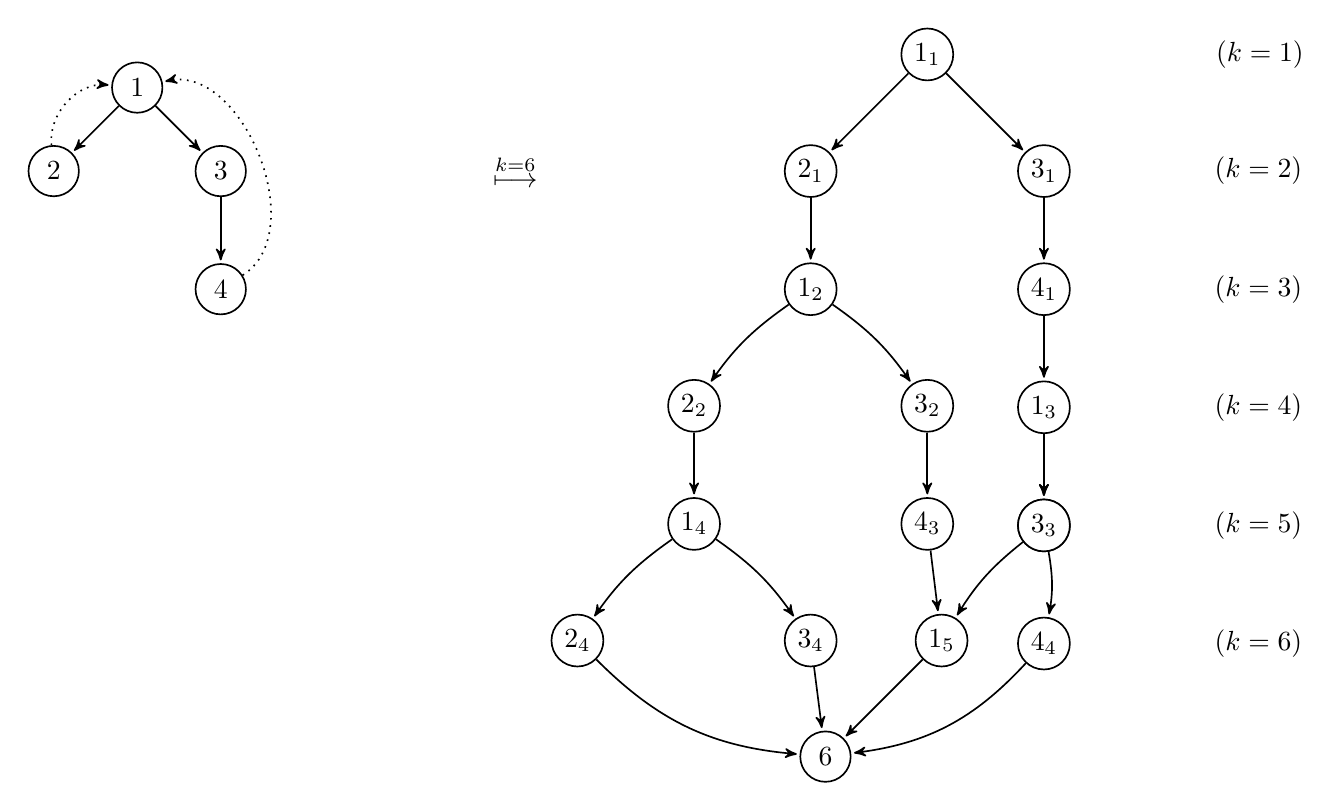
\begin{tikzpicture}[->,>=stealth',shorten >=1pt,auto,node distance=1.5cm,semithick]
\node[c] (1) [] {$1$};
\node[c] (2) [below left of=1] {$2$};
\node[c] (3) [below right of=1] {$3$};
\node[c] (4) [below of=3] {$4$};
\path[->]
(1) edge [] node {} (2)
(2) edge [bend left=50,dotted] node {} (1)
(1) edge [] node {} (3)
(3) edge [] node {} (4)
(4) edge [bend right=80,dotted] node {} (1)
;
\node[draw=none] (impl) [right=3cm of 3] {$\overset{k = 6}{\longmapsto}$};
;
\node[c] (21) [right=3cm of impl] {$2_1$};
\node[c] (11) [above right=1cm and 1cm of 21]{$1_1$};
\node[c] (31) [below right=1cm and 1cm of 11] {$3_1$};
\node[c] (41) [below of=31] {$4_1$};
\node[c] (12) [below of=21] {$1_2$};
\node[c] (22) [below left=1cm and 1cm of 12] {$2_2$};
\node[c] (32) [below right=1cm and 1cm of 12] {$3_2$};
\node[c] (13) [below of=41] {$1_3$};
\node[c] (14) [below of=22] {$1_4$};
\node[c] (43) [below of=32] {$4_3$};
\node[c] (23) [below of=13] {$2_3$};
\node[c] (33) [below of=13] {$3_3$};
\node[c] (24) [below left=1cm and 1cm of 14] {$2_4$};
\node[c] (34) [below right=1cm and 1cm of 14] {$3_4$};
\node[c] (15) [below right=1cm and -0.3cm of 43] {$1_5$};
\node[c] (44) [below of=33] {$4_4$};
\node[c] (6) [below left=1cm and 1cm of 15] {$6$};
\node[] (11k) [right=3.2cm of 11] {$(k = 1)$};
\node[] (31k) [right=1.7cm of 31] {$(k = 2)$};
\node[] (41k) [right=1.7cm of 41] {$(k = 3)$};
\node[] (13k) [right=1.7cm of 13] {$(k = 4)$};
\node[] (33k) [right=1.7cm of 33] {$(k = 5)$};
\node[] (44k) [right=1.7cm of 44] {$(k = 6)$};
\path[->]
(11) edge [] node {} (21)
(11) edge [] node {} (31)
(31) edge [] node {} (41)
(21) edge [] node {} (12)
(12) edge [bend right=10] node {} (22)
(12) edge [bend left=10] node {} (32)
(41) edge [] node {} (13)
(22) edge [] node {} (14)
(32) edge [] node {} (43)
(13) edge [] node {} (23)
(13) edge [] node {} (33)
(14) edge [bend right=10] node {} (24)
(14) edge [bend left=10] node {} (34)
(43) edge [] node {} (15)
(33) edge [bend right=10] node {} (15)
(33) edge [bend left=10] node {} (44)
(24) edge [bend right=20] node {} (6)
(34) edge [] node {} (6)
(15) edge [] node {} (6)
(44) edge [bend left=20] node {} (6)
;
\end{tikzpicture}
\caption{Example of the flow graph from Figure~\ref{fig:merged-loop}, unwinded up to the bound $k = 6$} \label{fig:merged-loop}
\end{figure}

\end{document}

" 
\ifdefined\IsAalto
  def
\else
  non-def
\fi

\begin{figure}
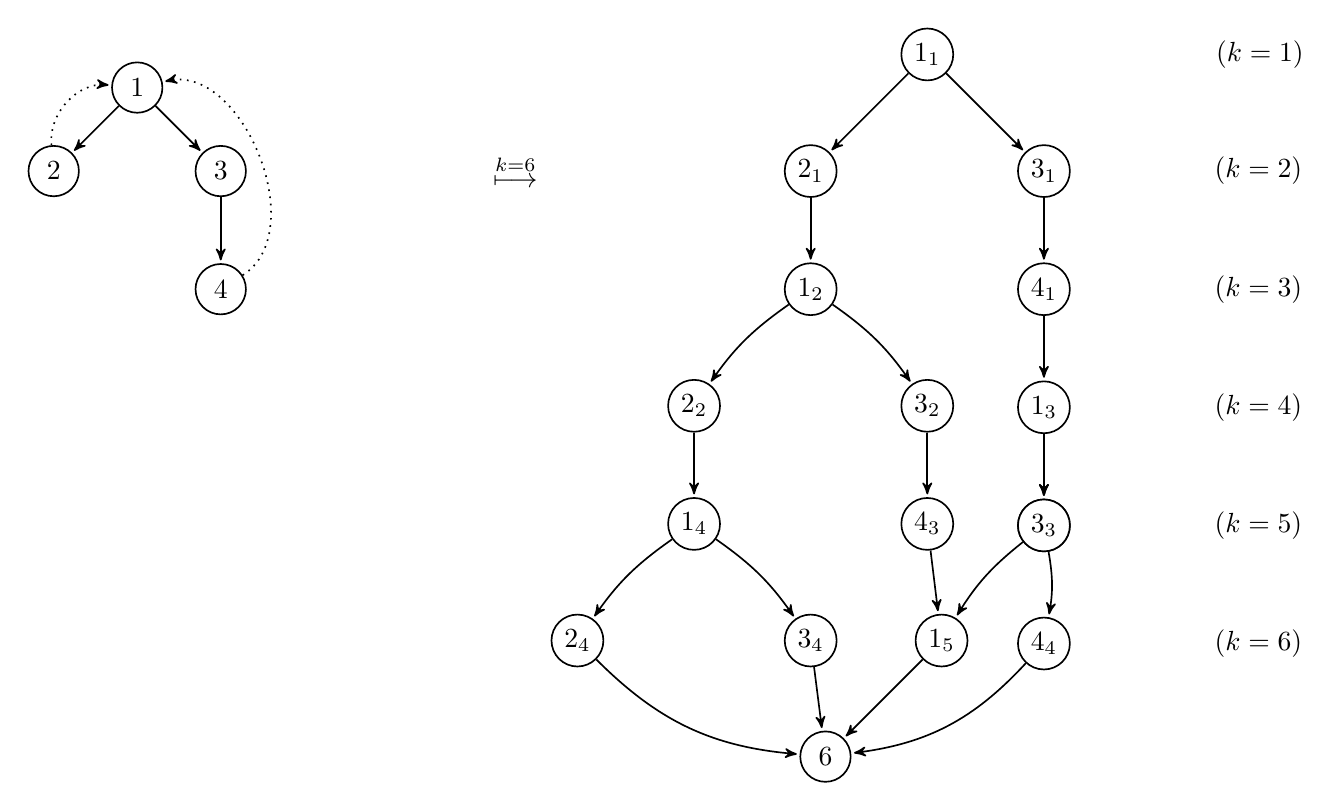
\begin{tikzpicture}[->,>=stealth',shorten >=1pt,auto,node distance=1.5cm,semithick]
\node[c] (1) [] {$1$};
\node[c] (2) [below left of=1] {$2$};
\node[c] (3) [below right of=1] {$3$};
\node[c] (4) [below of=3] {$4$};
\path[->]
(1) edge [] node {} (2)
(2) edge [bend left=50,dotted] node {} (1)
(1) edge [] node {} (3)
(3) edge [] node {} (4)
(4) edge [bend right=80,dotted] node {} (1)
;
\node[draw=none] (impl) [right=3cm of 3] {$\overset{k = 6}{\longmapsto}$};
;
\node[c] (21) [right=3cm of impl] {$2_1$};
\node[c] (11) [above right=1cm and 1cm of 21]{$1_1$};
\node[c] (31) [below right=1cm and 1cm of 11] {$3_1$};
\node[c] (41) [below of=31] {$4_1$};
\node[c] (12) [below of=21] {$1_2$};
\node[c] (22) [below left=1cm and 1cm of 12] {$2_2$};
\node[c] (32) [below right=1cm and 1cm of 12] {$3_2$};
\node[c] (13) [below of=41] {$1_3$};
\node[c] (14) [below of=22] {$1_4$};
\node[c] (43) [below of=32] {$4_3$};
\node[c] (23) [below of=13] {$2_3$};
\node[c] (33) [below of=13] {$3_3$};
\node[c] (24) [below left=1cm and 1cm of 14] {$2_4$};
\node[c] (34) [below right=1cm and 1cm of 14] {$3_4$};
\node[c] (15) [below right=1cm and -0.3cm of 43] {$1_5$};
\node[c] (44) [below of=33] {$4_4$};
\node[c] (6) [below left=1cm and 1cm of 15] {$6$};
\node[] (11k) [right=3.2cm of 11] {$(k = 1)$};
\node[] (31k) [right=1.7cm of 31] {$(k = 2)$};
\node[] (41k) [right=1.7cm of 41] {$(k = 3)$};
\node[] (13k) [right=1.7cm of 13] {$(k = 4)$};
\node[] (33k) [right=1.7cm of 33] {$(k = 5)$};
\node[] (44k) [right=1.7cm of 44] {$(k = 6)$};
\path[->]
(11) edge [] node {} (21)
(11) edge [] node {} (31)
(31) edge [] node {} (41)
(21) edge [] node {} (12)
(12) edge [bend right=10] node {} (22)
(12) edge [bend left=10] node {} (32)
(41) edge [] node {} (13)
(22) edge [] node {} (14)
(32) edge [] node {} (43)
(13) edge [] node {} (23)
(13) edge [] node {} (33)
(14) edge [bend right=10] node {} (24)
(14) edge [bend left=10] node {} (34)
(43) edge [] node {} (15)
(33) edge [bend right=10] node {} (15)
(33) edge [bend left=10] node {} (44)
(24) edge [bend right=20] node {} (6)
(34) edge [] node {} (6)
(15) edge [] node {} (6)
(44) edge [bend left=20] node {} (6)
;
\end{tikzpicture}
\caption{Example of the flow graph from Figure~\ref{fig:merged-loop}, unwinded up to the bound $k = 6$} \label{fig:merged-loop}
\end{figure}

\end{document}

" 
\ifdefined\IsAalto
  def
\else
  non-def
\fi

\begin{figure}
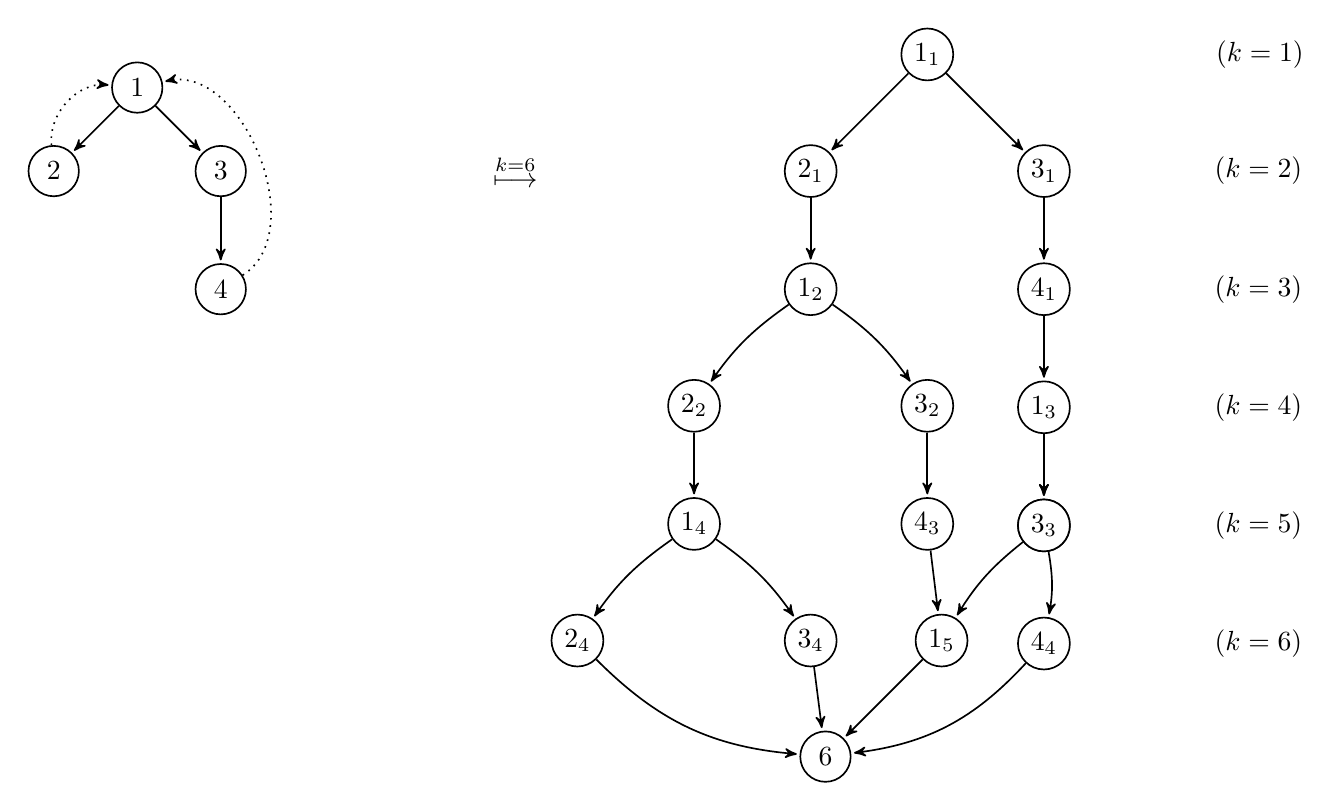
\begin{tikzpicture}[->,>=stealth',shorten >=1pt,auto,node distance=1.5cm,semithick]
\node[c] (1) [] {$1$};
\node[c] (2) [below left of=1] {$2$};
\node[c] (3) [below right of=1] {$3$};
\node[c] (4) [below of=3] {$4$};
\path[->]
(1) edge [] node {} (2)
(2) edge [bend left=50,dotted] node {} (1)
(1) edge [] node {} (3)
(3) edge [] node {} (4)
(4) edge [bend right=80,dotted] node {} (1)
;
\node[draw=none] (impl) [right=3cm of 3] {$\overset{k = 6}{\longmapsto}$};
;
\node[c] (21) [right=3cm of impl] {$2_1$};
\node[c] (11) [above right=1cm and 1cm of 21]{$1_1$};
\node[c] (31) [below right=1cm and 1cm of 11] {$3_1$};
\node[c] (41) [below of=31] {$4_1$};
\node[c] (12) [below of=21] {$1_2$};
\node[c] (22) [below left=1cm and 1cm of 12] {$2_2$};
\node[c] (32) [below right=1cm and 1cm of 12] {$3_2$};
\node[c] (13) [below of=41] {$1_3$};
\node[c] (14) [below of=22] {$1_4$};
\node[c] (43) [below of=32] {$4_3$};
\node[c] (23) [below of=13] {$2_3$};
\node[c] (33) [below of=13] {$3_3$};
\node[c] (24) [below left=1cm and 1cm of 14] {$2_4$};
\node[c] (34) [below right=1cm and 1cm of 14] {$3_4$};
\node[c] (15) [below right=1cm and -0.3cm of 43] {$1_5$};
\node[c] (44) [below of=33] {$4_4$};
\node[c] (6) [below left=1cm and 1cm of 15] {$6$};
\node[] (11k) [right=3.2cm of 11] {$(k = 1)$};
\node[] (31k) [right=1.7cm of 31] {$(k = 2)$};
\node[] (41k) [right=1.7cm of 41] {$(k = 3)$};
\node[] (13k) [right=1.7cm of 13] {$(k = 4)$};
\node[] (33k) [right=1.7cm of 33] {$(k = 5)$};
\node[] (44k) [right=1.7cm of 44] {$(k = 6)$};
\path[->]
(11) edge [] node {} (21)
(11) edge [] node {} (31)
(31) edge [] node {} (41)
(21) edge [] node {} (12)
(12) edge [bend right=10] node {} (22)
(12) edge [bend left=10] node {} (32)
(41) edge [] node {} (13)
(22) edge [] node {} (14)
(32) edge [] node {} (43)
(13) edge [] node {} (23)
(13) edge [] node {} (33)
(14) edge [bend right=10] node {} (24)
(14) edge [bend left=10] node {} (34)
(43) edge [] node {} (15)
(33) edge [bend right=10] node {} (15)
(33) edge [bend left=10] node {} (44)
(24) edge [bend right=20] node {} (6)
(34) edge [] node {} (6)
(15) edge [] node {} (6)
(44) edge [bend left=20] node {} (6)
;
\end{tikzpicture}
\caption{Example of the flow graph from Figure~\ref{fig:merged-loop}, unwinded up to the bound $k = 6$} \label{fig:merged-loop}
\end{figure}

\end{document}

" 
\ifdefined\IsAalto
  \documentclass[12pt,a4paper,oneside,pdftex]{report}
  \usepackage[doublenumbering,twosupervisors]{lib/aalto-thesis}
\else
  \documentclass[14pt,a4paper,oneside,pdftex]{extreport}
  \usepackage{lib/itmo-thesis}
\fi


% Bibliography
\addbibresource{bib/ms-thesis.bib}

\newcommand{\TITLE}{\nohyphens{Automated Analysis of Weak Memory Models}}
%\newcommand{\FTITLE}{?}
%\newcommand{\FSUBTITLE}{}
%\newcommand{\FDATE}{?.?.2018} % TODO
\newcommand{\SUBTITLE}{}
\newcommand{\DATE}{18.6.2018}

% Supervisors and instructors
% ------------------------------------------------------------------
% If you have two supervisors, write both names here, separate them with a
% double-backslash (see below for an example)
% Also remember to add the package option ``twosupervisors'' or
% ``twoinstructors'' to the aalto-thesis package so that the titles are in
% plural.
% Example of one supervisor:
\newcommand{\SUPERVISOR}{Assoc. Prof. Keijo Heljanko\\Docent Igor I. Komarov}
%\newcommand{\FSUPERVISOR}{} % TODO
%\newcommand{\SSUPERVISOR}{} % TODO

% If you have only one instructor, just write one name here
%\newcommand{\INSTRUCTOR}{} % TODO
%\newcommand{\FINSTRUCTOR}{} % TODO
%\newcommand{\SINSTRUCTOR}{} % TODO
% If you have two instructors, separate them with \\ to create linefeeds
% \newcommand{\INSTRUCTOR}{Olli Ohjaaja M.Sc. (Tech.)\\
%  Elli Opas M.Sc. (Tech)}
%\newcommand{\FINSTRUCTOR}{Diplomi-insinööri Olli Ohjaaja\\
%  Diplomi-insinööri Elli Opas}
%\newcommand{\SINSTRUCTOR}{Diplomingenjör Olli Ohjaaja\\
%  Diplomingenjör Elli Opas}

% If you have two supervisors, it is common to write the schools
% of the supervisors in the cover page. If the following command is defined,
% then the supervisor names shown here are printed in the cover page. Otherwise,
% the supervisor names defined above are used.
%\newcommand{\COVERSUPERVISOR}{Professor Antti Ylä-Jääski, Aalto University\\
%  Professor Pekka Perustieteilijä, University of Helsinki}

% The same option is for the instructors, if you have multiple instructors.
% \newcommand{\COVERINSTRUCTOR}{Olli Ohjaaja M.Sc. (Tech.), Aalto University\\
%  Elli Opas M.Sc. (Tech), Aalto SCI}


% Other stuff
% ------------------------------------------------------------------
%\newcommand{\PROFESSORSHIP}{} % TODO
%\newcommand{\FPROFESSORSHIP}{?} % TODO check
% Professorship code is the same in all languages
%\newcommand{\PROFCODE}{AS-116} % TODO check
\newcommand{\KEYWORDS}{Weak memory models, concurrent programming, software verification, portability analysis, bounded reachability analysis, SMT-encoding}
%\newcommand{\FKEYWORDS}{Diplomityöpohja} % TODO
\newcommand{\LANGUAGE}{English}
%\newcommand{\FLANGUAGE}{Englanti} % TODO

% Author is the same for all languages
\newcommand{\AUTHOR}{Artem Yushkovskiy}


% Currently the English versions are used for the PDF file metadata
% Set the PDF title
\hypersetup{pdftitle={\TITLE\ \SUBTITLE}}
% Set the PDF author
\hypersetup{pdfauthor={\AUTHOR}}
% Set the PDF keywords
\hypersetup{pdfkeywords={\KEYWORDS}}
% Set the PDF subject
\hypersetup{pdfsubject={Master's Thesis}}


% Layout settings
% ------------------------------------------------------------------

% When you write in English, you should use the standard LaTeX
% paragraph formatting: paragraphs are indented, and there is no
% space between paragraphs.
% When writing in Finnish, we often use no indentation in the
% beginning of the paragraph, and there is some space between the
% paragraphs.

% If you write your thesis Finnish, uncomment these lines; if
% you write in English, leave these lines commented!
%\setlength{\parindent}{0pt}
%\setlength{\parskip}{1ex}

% Use this to control how much space there is between each line of text.
% 1 is normal (no extra space), 1.3 is about one-half more space, and
% 1.6 is about double line spacing.
\ifdefined\IsAalto
  \linespread{1.05} %almost single spacing 
\else
  \linespread{1.3}%one-and-a-half spacing
  %\setlength{\parindent}{1.25cm} %горизонтальн
  \setlength{\parskip}{0pt} %вертикальн
%  \renewcommand{\baselinestretch}{1} %между параграфами 
\fi
% \linespread{1.25}

% Extra hyphenation settings
% ------------------------------------------------------------------
% You can list here all the files that are not hyphenated correctly.
% You can provide many \hyphenation commands and/or separate each word
% with a space inside a single command. Put hyphens in the places where
% a word can be hyphenated.
% Note that (by default) LaTeX will not hyphenate words that already
% have a hyphen in them (for example, if you write ``structure-modification
% operation'', the word structure-modification will never be hyphenated).
% You need a special package to hyphenate those words.
%\hyphenation{di-gi-taa-li-sta}


% Proper style for book binding, left margin bigger than right margin
% Uncomment to take into use
%\setlength{\parindent}{0pt}
%\setlength{\parskip}{2ex}
%\setlength{\textwidth}{140mm}
%\setlength{\oddsidemargin}{20mm}
%\setlength{\evensidemargin}{20mm}
%\setlength{\textheight}{240mm}
%\setlength{\voffset}{3mm}
%\setlength{\topmargin}{-11mm}


%\definecolor{pblue}{rgb}{0.13,0.13,1}
%\definecolor{pgreen}{rgb}{0,0.5,0}
%\definecolor{pred}{rgb}{0.9,0,0}
%\definecolor{pgrey}{rgb}{0.46,0.45,0.48}
%\lstset{
%  showspaces=false,
%  showtabs=false,
%  breaklines=true,
%  showstringspaces=false,
%  breakatwhitespace=true,
%  commentstyle=\color{pgreen},
%  keywordstyle=\color{pblue},
%  stringstyle=\color{pred},
%  basicstyle=\ttfamily\scriptsize,
%  moredelim=[il][\textcolor{pgrey}]{$$},
%  moredelim=[is][\textcolor{pgrey}]{\%\%}{\%\%}
%}

% The preamble ends here, and the document begins.
% Place all formatting commands and such before this line.
% ------------------------------------------------------------------
\begin{document}



% This command adds a PDF bookmark to the cover page
\pdfbookmark[0]{Cover}{bookmark.0.cover}

\startcoverpage

% Cover page
% ------------------------------------------------------------------
% Options: finnish, english, and swedish
\coverpage{english}

%change page numbering:
%\if 
%\addtocounter{page}{1}

% Abstract in English
% ------------------------------------------------------------------
\thesisabstract{english}{
Software verification is considered to be a hard computational problem vulnerable to the state explosion problem.
Concurrent software verification raises the complexity of the problem to a power determined by %by the factor defined
all the possible interleavings of states of the system. %concurrent parts of the system.
Moreover, the architecture of a modern shared-memory multi-core processor and optimisations performed by a compiler can cause program behaviour that is unexpected from the point of view of traditional concurrency.
The guarantees that an execution environment can provide to a programmer are formalised in its \textit{Weak Memory Model (WMM)}.
%The formalisation of weak memory models
Over the last decade, weak memory models were defined for multiple hardware architectures and programming languages.
%Thus, the memory model-aware software analysis 
%This opens/brings new 
%This opens new challenges in developing new and adapting existing methods for software verification with respect to a memory model.
This opens new challenges in software verification with respect to a weak memory model.
%Moreover, a modern shared-memory multiprocessor architecture or an optimising compiler can cause new program behaviours, unexpected from the point of view of traditional concurrency.
%These behaviours are described by the formal \textit{weak memory model} of an execution environment. %a processor architecture. % or a programming language.
%This opens large opportunities for missing bugs that are extremely difficult to reproduce and eliminate.
%formally described by <wmms> : guarantees even with aggressive hw and compiler optimisations

Most existing tools that perform memory model-aware software analysis tools examine behaviours of the program against a single memory model.
%Generally, they perform static 
%finite-state system
The first tool that analyses the \textit{portability} of a concurrent program from one platform to another is \textit{\porthos{}}~\cite{Porthos17a} released in April~2017.
\porthos{} can verify that the program is portable from the source platform $\mathcal{S}$ to the target platform $\mathcal{T}$ by checking that the program has no extra states under $\mathcal{T}$.
For that, it performs an SMT-based bounded reachability analysis by encoding the constraints of the program and two memory models $\mathcal{M_S}$ and $\mathcal{M_T}$ into a single SMT-formula.

Although the approach has been proven to be efficient, the tool accepts as input the small C-like toy language. % and remains to have hardly extensible architecture. %proof-of-concept 
Current thesis aims to rework \porthos{} by extending its input language, so that it is able to process real-world C programs.
However, current implementation of \porthos{} can be considered hardly extensible, which raises the need to redesign its whole architecture in order to increase the robustness, transparency, efficiency and extensibility.
The result of the work is \textit{\porthos[2]}, a framework for SMT-based memory model-aware analysis.
%to redesign \porthos{} so that 
%considers the problem of the memory model-aware program verification, especially verification the portability from one architecture to another.
%The main goal of the work was to rework the proof-of-concept tool \porthos{}, <extend the input lang>, rework architecture towards the framework for analysis of C 
}

% Acknowledgements
% ------------------------------------------------------------------
% Select the language you use in your acknowledgements
\selectlanguage{english}
% Uncomment this line if you wish acknoledgements to appear in the table of contents
%\addcontentsline{toc}{chapter}{Acknowledgements}

\chapter*{Acknowledgements}
First of all, I wish to thank Professor Keijo Heljanko for his continuous support in both technical and mental aspects of the work.
He has opened for me the opportunity of working in this extremely interesting project; he guided and assisted me during six months, explaining all the things I don't understand and helping to find the way when I have lost it.

Also, I feel grateful to the development team of the static analyser Application Inspector by Positive Technologies, where I've been working in~2016-17.
This was an important experience for me, there I learned how the high-class code analysers look like.
Especially I want to thank Vladimir Kochetkov who has a gift of explaining the complex matter in simplest words, and Stanislav Matveev who has taught me how to be a perfectionist in writing the code.

Although I did far not all things that I could have done, I learned a lot during the work on this project: about the compilation theory and logic, about concurrency and programming, and, most importantly, about myself.


\vskip 10mm

\noindent %\ATCITY
Espoo, Finland \newline
Saint Petersburg, Russia
\newline
\DATE
\vskip 5mm
\noindent \AUTHOR


% ------------------------------------------------------------------
% Use \cleardoublepage so that IF two-sided printing is used
% (which is not often for masters theses), then the pages will still
% start correctly on the right-hand side.
\cleardoublepage


\ifdefined\IsAalto
  \addcontentsline{toc}{chapter}{Abbreviations}
  \chapter*{Abbreviations}
% The longtable environment should break the table properly to multiple pages, if needed
\noindent
\begin{longtable}{@{}p{0.25\textwidth}p{0.7\textwidth}@{}}
API & Application Programming Interface \\
AST & Abstract Syntax Tree \\
BDD & Binary Decision Diagrams \\
BNF & Backus-Naur form \\
BMC & Bounded Model Checking \\
CF  & Control-Flow \\
CPU & Central Processor Unit \\
CTL & Computational Tree Logic \\
DF  & Data-Flow \\
DFS & Deep-First Search \\
DSA & Dynamic Single-Assignment form \\
DTO & Data-Transfer Object \\
LTL & Linear Temporal Logic \\
NP  & Non-deterministic Polynomial time \\
OOP & Object-Oriented Programming \\
SB  & Store Buffering \\
SC  & Sequential Consistency \\
SAT & Satisfiability problem \\
SMP & Symmetric Multiprocessor architecture \\
SMT & Satisfiability Modulo Theories problem \\
SSA & Static Single-Assignment form \\
UMC & Unbounded Model Checking \\
UML & Unified Modeling Language \\
WMM & Weak Memory Model \\
\end{longtable}

\else
\fi


% Table of contents
% ------------------------------------------------------------------
\cleardoublepage
% This command adds a PDF bookmark that links to the contents.
% You can use \addcontentsline{} as well, but that also adds contents
% entry to the table of contents, which is kind of redundant.
% The text ``Contents'' is shown in the PDF bookmark.
\pdfbookmark[0]{Table of contents}{bookmark.0.contents}
\tableofcontents

% List of tables
% ------------------------------------------------------------------
% You only need a list of tables for your thesis if you have very
% many tables. If you do, uncomment the following two lines.
%\cleardoublepage
%\listoftables

% Table of figures
% ------------------------------------------------------------------
% You only need a list of figures for your thesis if you have very
% many figures. If you do, uncomment the following two lines.
\cleardoublepage
%\phantomsection


\ifdefined\IsAalto
  \addcontentsline{toc}{chapter}{\listfigurename}
  \listoffigures
\else
\fi





% ===================================================================



% The following label is used for counting the prelude pages 
%https://latex.org/forum/viewtopic.php?t=21520 :
%\phantomsection %does not work either
%\newcounter{dummy}\refstepcounter{dummy}

\label{pages-prelude}

\cleardoublepage


%%%%%%%%%%%%%%%%% The main content starts here %%%%%%%%%%%%%%%%%%%%%
% ------------------------------------------------------------------
% This command is defined in aalto-thesis.sty. It controls the page
% numbering based on whether the doublenumbering option is specified
\startfirstchapter


% The contents of the thesis are separated to their own files.
% Edit the content in these files, rename them as necessary.
% ------------------------------------------------------------------


\chapter{Introduction}
\label{ch:intro}

Most modern computer systems contain large parts that operate concurrently. Though parallelisation of the system can improve its performance drastically, it opens numerous of problems connected to correctness, robustness and reliability, which makes the concurrent program design one of the most difficult problems of programming~\cite{mckenney2017parallel}.
% Most articles, presentations and books on concurrent programming start with words how hard it is.

Traditionally, studies related to concurrent programming concern on more fundamental theoretical questions of designing race-free and lock-free parallel algorithms, asynchronous data structures and synchronisation primitives of a programming language. Unfortunately,
when it comes to 
%in cases of 
the real-world concurrent programs, the algorithmic level of abstraction is not enough for guaranteeing their properties of correctness and reliability. The reasons of this fact lie in the code optimisations that both compiler and hardware perform in order to increase performance as much as possible. For instance, Figure~\ref{simple_wmm_x86} provides simple example of
unexpected state `\texttt{(0:EAX=0~/\textbackslash~1:EAX=0)}' reachable on x86 machines (such little examples that illustrate specific behaviour of a WMM are called \textit{litmus tests}).
%reordering of memory access instructions within single process allowed by the x86-TSO weak memory model, which potentially breaks the program logic. 
This state is allowed because in x86 architecture each processor may cache the write to shared memory variable into its local write buffer, so that they do not become visible by other processes immediately. In the example, the write `\texttt{MOV~[x],1}' performed by process \texttt{P0} stores value~\texttt{1} to the shared variable~\texttt{[x]} into the write buffer of process~\texttt{P0}. Meanwhile, the write cache of the process \texttt{P1} may not have updated version of the variable~\texttt{[x]}, neither may have the main memory, so that the read `\texttt{MOV~EBX,[x]}' performed in the process~\texttt{P1} may read the initial value~\texttt{0}, even if this variable has been already updated in another thread.
%More presice description of x86-TSO memory model is given in Chapter~\ref{ch:wmm:x86}.

\begin{figure}
\small \ttfamily
\begin{tabular}{ |l|l| }
\hline
\multicolumn{2}{|l|}{ \{ x=0; y=0; \}} \tabularnewline \hline
P0 & P1 \\ \hline
MOV [x],1 & MOV [y],1 \\
MOV EAX,[y] & MOV EAX,[x] \\
\hline
%\multicolumn{2}{|l|}{locations [x;y;]} \tabularnewline
\multicolumn{2}{|l|}{exists (0:EAX=0~/\textbackslash~1:EAX=0)} \tabularnewline
\hline
\multicolumn{2}{|l|}{x86-TSO: allow} \tabularnewline
\hline

\end{tabular}
\caption{Store buffering (SB): a test on write-read reordering allowed under the x86-TSO weak memory model}
\label{simple_wmm_x86}
\end{figure}

The first memory model for concurrent systems was formulated by Leslie Lamport back in 1979~\cite{lamport1979make}. This memory model, called the \textit{sequential consistency (SC)}, allows only those executions (interleavings) that produce the same result as if the operations had been executed by single process. This means that the order of operations executed by a process is strictly defined by the program it executes. The SC model does requires the write to a shared variable performed in one process to become visible by all other processes not instantly, but simultaneously. This means each process communicates to the shared memory directly, without local buffering. Another important requirement of SC memory model is that it forbids memory operations reordering within single process (the order is strictly defined by the program).

The SC model is considered to be the strong memory model in the sence that it provides strong guarantees regarding the ordering and caused effect of memory operations. Different relaxations of this model lead to the class of \textit{weak memory models~(WMM)}.
%while preserving consistency
They specify how threads interact through shared memory, when a write becomes visible to other threads and what value a read can return. 
Therefore, WMMs serve as set of guarantees made by designers of execution environment (hardware, programming language, compiler, database, operation system, etc.) to programmers on which behaviours of their concurrent code they may expect. 

Although weak memory studies is rather young research area, there exist frameworks and tools for exploring WMMs and examining simple programs with respect to the them. The state-of-the-art tool is \tool{diy} (for \textit{do it yourself}), developed by the researchers from INRIA institute, France and University of Cambridge, UK.
The \tool{diy}\footnote{\url{diy.inria.fr}} is a sofware suite for designing and testing weak memory models. It is firstly released back in 2010, and since that time it remained to be the only tool for testing weak memory models. The \tool{diy} consists of several modules: the litmus tests generators \tool{diy7}, \tool{diycross7} and \tool{diyone7}, the litmus tests concrete executor \tool{litmus7} that runs tests on a physical machine while collecting its behaviours, and the weak memory models simulator \tool{herd7} that implements reachability analysis for exploring states reachable under specified~WMM.

All the \tool{diy} tools work only with single memory model, however, in real life we face serious engineering problems involving necessity to model more than one execution environment. One of these problems is the \textit{portability} of the program from one hardware architecture to another. A program written in a high-level language is then compiled for different hardware. Even if all the compiler optimisations were disabled (which is rare case nowadays), the behaviour of two compiled versions of the same program may differ due to differences between hardware memory models. As the result, the program compiled for the platform $X$, can reach states that are unreachable on the platform $Y$, or some states that are reachable on $Y$ can become unreachable on $X$. We declare these cases as \textit{portability bugs}.

The first tool that performs the WMM-awared portability analysis is \tool{PORTHOS} introduced in April~2017~\cite{Porthos17}. This tool reduces described problem to a bounded reachability problem, which can be solved with help of an SMT-solver. This approach allows to capture symbolically the semantics of analysing program and both weak memory models into single SMT-formula, augmented by the reachability assertion. As most modern SMT-solvers are efficient enough to be able to operate the state space of size millions of variables bounded by millions of constraints~(\cite{malik2009boolean}), the used method can be applicable in solving the real-world problems.
% TODO: search space size: https://courses.cs.washington.edu/courses/csep573/11wi/lectures/ashish-satsolvers.pdf slide 

%In the work~\cite{Porthos17}, the SMT-based approach was defined for analysing the portability of a program from one hardware architechture to another, which is defined as ``an execution that is consistent with the target but inconsistent with the source memory model". Although encoding the control-flow and the data-flow of a program into an SMT-formula seems to be a trivial problem of symbolic execution, encoding of the weak memory model is more tedious. The reason is that some relations of WMMs are defined as mutually-recursive and need to be linearised in order to be encoded into an equivalent logical formula.

%"A portability bug is an execution that is consistent with the target but inconsistent with the source memory model. We capture this alternation with a single existential query. Consistency is specified in terms of acyclicity (and irreflexivity) of relations. Hence, an execution is inconsistent if a derived relation of the (source) memory model contains a cycle (or is not irreflexive)."

Current work aims to rework the proof-of-concept tool \tool{PORTHOS} by extending the input language, which currently represents the minimum subset of C, and revising the general architecture of the tool in order to enhance performance, reliability and mantainability.
%interprocedural analysis
We called the new tool \textbf{the \tool{mousquetaires} framework} as now it not only performs the portability analysis, but can serve as the basis for SMT-solver driven weak memory model analysis.

\section{Thesis structure}
\label{ch:intro:structure}

The Chapter~\ref{ch:wmm} gives more detailed description of the weak memory model-awared analysis and provides description of memory models for some common architectures (x86, ARM and POWER, Sparc, ???). Chapter~...

% TODO: Add intro to the bounded reachability analysis using SAT -- ? 
\chapter{Memory model-aware analysis}
\label{ch:wmm}

The main idea behind the memory model-aware program analysis is that the set of all possible interleavings of the concurrent program (\textit{anarchic semantics}) can be specified by the axiomatic constraints of the memory model that filter out executions inconsistent in particular architecture (\textit{analytic semantics})~\cite{alglave2016syntax}.
The anarchic semantics of the program is a truly parallel semantics with no global time that describes all possible computations with all possible communications.
However, the analytic semantics captures the program behaviours on a certain execution environment more precisely.
%"The semantics of a program is a set of executions" https://johnwickerson.github.io/papers/memalloy.pdf


\section{The event-based program representation}
\label{ch:wmm:event}

The classical approach for analysing concurrent programs is to model it as the set of sequentially consistent programs, obtained by enumerating all possible interleavings.
These models are deterministic as they include the notion of the \textit{global time}. %, a single order of interleavings among all events happened in different threads.
Although these models are easy to build and analyse, the number of all possible interleavings grows exponentially (known as the \textit{combinatorial explosion}), which affects the completeness of an analysis method in general case.

One way to fight the combinatorial explosion is to exclude the global time from the model and treat executions from one equivalence class together in a non-deterministic fashion.
For instance, such an equivalence class can be the set of computations performed by a processor locally that do not affect the global state.
This idea is used in the \textit{event-based} model, that represents the program as a directed graph of events (the \textit{event-flow graph})~\cite{alglave2010shared}.
The vertices of such a graph represent \textit{events} (see Section~\ref{ch:wmm:model:events}), and edges represent basic relations (see Section~\ref{ch:wmm:model:relations}).
The graph represents the set of executions (sequences of events; see Section~\ref{ch:wmm:model:executions}) defined by the non-deterministic guesses of certain relations on some states.

There are three main types of sources of non-determinism in concurrent programs~\cite{musuvathi2008fair}:
\begin{enumerate}[noitemsep,topsep=0pt]
\item \textit{input non-determinism}, which is a standard undecidable problem for all static analysis methods: to resolve the user input, system call from the environment, unresolved function calls, etc.;
\item \textit{scheduling non-determinism}, caused by the interleavings, which in turn are caused by the scheduler activity;
\item \textit{memory-model non-determinism}, caused by hardware and compiler relaxations.
\end{enumerate}

The event-based program model is able to emulate effectively the second and the third types of sources of non-determinism, while the first one can be coped by standard static analysis methods~\cite{landi1992undecidability,SurveySymExec-CSUR18}.

%- The semantics of the event-flow graph is given:  "alglave: Don’t sit on the fence A static analysis approach to automatic fence insertion" page 8 or 9
%"To build the aeg , we define a semantics of goto-programs in terms of abstract events, ..."
% TODO: OR from here: http://www.cprover.org/etaps/esop.pdf "Software Verification for Weak Memory via Program Transformation"


\subsection{Events}
\label{ch:wmm:model:events}

%TODO: EVENT -- ATOMIC?
An event is a fact of executing the low-level primitive operation such as memory access, threads synchronisation, computation, etc.

A \textit{memory event} $e_m \in \mathbb{E}$ represents the fact of access to the memory.
Only memory events change the state of an abstract machine executing the code, since it is completely determined by values stored in its memory.
Since memory is the crucial low-level resource shared by multiple processes, most relations are defined over memory events. 
The processes can access a shared memory location (denoted by~$l_i$, for \textit{location}), or a local one (denoted by~$r_i$, for \textit{register}).
A memory event can access at most one shared memory location, high-level instructions that address more than one shared variable must be transformed into a sequence of events.
A memory event is specified by its direction with respect to the shared variable, its location~$\mathtt{loc}(e_m)$, its processor label~$\mathtt{proc}(e_m)$, and a unique event label~$\mathtt{id}(e_m)$~\cite{alglave2010shared}.
%\texttt{load} for read the value of a shared-memory location, or \texttt{store} for write, or neither of them if both locations are local

The set of memory events $\mathbb{M}$ is divided into write events $\mathbb{W}$ (that write values to shared-memory locations) and read events $\mathbb{R}$ (that read values stored in shared-memory locations).
We add a restriction that each memory event uses at most one shared location, so that the write instruction $i = write(l_1, l_2)$, that encodes the write from the shared location $l_2$ to the shared location $l_1$, is represented as two consequent events $e_1~=~\mathtt{load}(r_1~\leftarrow~l_2); \ e_2~=~\mathtt{store}(l_1~\leftarrow~r_1)$.
Also, it is important to separate the set of initial write events $\mathbb{IW}~\subseteq~\mathbb{W}$ that perform initialisation of program variables.

A \textit{computation event} $e_c \in \mathbb{C} \subseteq \mathbb{E}$, represents a low-level assembly computation operation performed solely on local-memory arguments.
An example of computation event may be the event $e_c = r_1 \leftarrow add(r_2, 1)$ that writes the sum of values stored in register $r_2$ and constant $1$ (which is modelled as a register as well) to the register $r_1$.
For modelling branching statements, we define the set $\mathbb{C}_{g}~\subseteq~\mathbb{C}$ of \textit{guard} computation events (also called as \textit{branching events}), that are evaluated to a boolean value.

The synchronisation instructions (fences) cause the \textit{barrier events}, that do not perform any computation or memory value transfer, instead, they add new relations to the program model that restrict the set of allowed behaviours.
Functionally, a fence may be a synchronisation barrier or a instruction of flushing the local memory caches, etc.

% TODO: more fences: "On Power and ARM (see Sec. 6), we distinguish between control fence (which we write cfence), lightweight fence (lwfence) and full fence (ffence). On x86, implementing TSO, there is only one fence, called mfence." (herding cats, p. 14)

\subsection{Relations}
\label{ch:wmm:model:relations}

%In this section, we describe basic relations used in memory model-aware program analysis.

The relation~$r\,\subseteq~\mathbb{E}~\times~\mathbb{E}$ is a set of pairs of events (a subset of Cartesian product of two sets of events). There are two kinds of relations between events: \textit{basic relations} that capture the semantics of the program, and \textit{derived relations} that are defined from the basic relations and events in the weak memory model specification. Constraints over relations that are specified by weak memory models are defined as requirements of acyclicity, irreflexivity or emptiness of specific relations~\cite{alglave2016syntax}.

\vspace{1em}
The basic relations are the following~\cite{alglave2010shared}:
%TODO: say that po and rf are  defined from the candidate execution:
%TODO: say that 
\begin{itemize}
    \item The \textit{control-flow} of a program is defined by the \textit{program-order} relation \po~$\subseteq~\mathbb{E}~\times~\mathbb{E}$, which represents the total order of events of same process.
    For instance, if the instruction $i_1$ generates the event $e_1$ and the instruction $i_2$ follows $i_1$ and generates the event $e_2$, then $e_1 \relation{po} e_2$.
    %Some new relations may be acquired : dp, po-loc

    \item The \textit{data-flow} of a program is defined by \textit{communication relations}:
    \begin{itemize}[noitemsep]
        \item the \textit{read-from} relation \rf{}~$\subseteq~\mathbb{W}~\times~\mathbb{R}$ that maps each write event to the read event that reads the value written by write event;
        \item the \textit{coherence order} relation \co{}~$\subseteq~\mathbb{W}~\times~\mathbb{W}$ that defines the total order on writes to the same location across all processes (also called the \textit{write serialisation}, \texttt{ws}-relation);
    \end{itemize}

    \item Events from the same process are related by the \textit{scope relation} \sr{}~$\subseteq~\mathbb{E}~\times~\mathbb{E}$.
    In contrast to the \tool{herd} tool, the \porthos[2] does not use hierarchy of scopes (depicted as the scope tree); instead, it uses simple labels that indicate which process has produced certain event.
\end{itemize}

%TODO: add ppo = characteristics of memory model. "Architectures are instances of our model. An architecture is a triple of functions (ppo, fences, prop), which specifies the preserved program order ppo, the fences fences and the propagation order prop." (herding cats, p.13)

Below we enumerate some derived relations~\cite{alglave2010shared}:

\begin{itemize}

    \item the \textit{from-read} relation $\fr \subseteq~\mathbb{R}~\times~\mathbb{W}$ that maps a read event to all write events succeeding the write event from which the read event gets its value: \\
    $r \relation{fr} w ~\triangleq~ (\exists w' . w' \relation{rf} r \land w' \relation{co} w)$

    %\item the \textit{data dependency} relation \texttt{dp}, which is a subset of \po-relation that always has a read at its source (it connects the read to the write which it depends on)
    %TO-DO: formula for dp or exclude

    \item the \textit{communication} relation \com over memory events, that fully describes the data-flow of a program: \\
    %$\mathtt{com} \triangleq (\mathtt{rf} \cup \mathtt{co} \cup \mathtt{fr})$
    $m_1 \relation{com} m_2~\triangleq~((m_1\relation{rf}m_2) \lor (m_1\relation{co}m_2) \lor (m_1\relation{fr}m_2))$

    \item the \textit{external} (and \textit{internal}) \textit{from-read} relations that restrict the \fr-relation to the different (respectively, same) processes: \\
    $w \relation{fre} r ~\triangleq~ (w \relation{fr} r \land \mathtt{proc}(w) = \mathtt{proc}(w))$ \\
    $w \relation{fri} r ~\triangleq~ (w \relation{fr} r \land \mathtt{proc}(w) \neq \mathtt{proc}(w))$
    
    %TODO: say that po-relation is *static*
    \item the \texttt{po-loc} relation that is the \po-relation over events that access to the same shared variable: \\
    $m_1 \relation{po-loc} m_2 ~\triangleq~ (m_1 \relation{po} m_2 \land \mathtt{loc}(m_1) = \mathtt{loc}(m_2))$

    \item the semantics of \textit{fences} (memory barriers) specific for different architectures may be defined as derived relations.

    %"Preserved program order defines the set of reorderings guaranteed by the architecture not to occur, based on the types of the accesses." http://delivery.acm.org/10.1145/2750000/2742219/p635-lustig.pdf

\end{itemize}

%todo: some words here?


\subsection{Executions}
\label{ch:wmm:model:executions}

The semantics of a concurrent program is represented as the set of allowed executions.
The \textit{execution} is a path in the event-flow graph defined by \po- and \rf-relations and set of final writes to a given memory location that is valid under certain memory model~\cite{alglave2014herding}.
It can be interpreted as a sequence of guesses which event is to be executed next.
The \textit{candidate execution} is an execution that is not yet constrained by a memory model.

%TODO: cite this paper elsewhere
%As it was shown in~\cite{wickerson2017automatically}, it is enough for memory models to constrain the executions independently instead of constraining the program at a whole.

%An \textit{execution} (trace, run) of a program is an ordered set of events defined by \po- and \rf-relations and set of final writes to a given memory location that is valid under certain memory model~\cite{alglave2014herding}.
%The order of events in particular execution is denoted as `$\rightarrow$', an empty execution is denoted as $\emptyset$.
%associated with the instructions of the program
%An execution is considered to be \textit{valid} if the memory events follow a single global timeline, i.e., can be embedded in a single partial order allowed by the memory model restrictions~\cite{alglave2010shared}.
%An execution is uniquely defined by the set $\mathbb{X}$ of events have been executed in each thread (the \textit{control-flow} of a program), and the relations $\mathtt{rf}$ and $\mathtt{co}$~\cite{alglave2010shared}.
Figure~\ref{simple_wmm_x86_pic} illustrates four possible candidate executions for the litmus test Example~\ref{simple_wmm_x86} (the pictures are generated by the \tool{herd7} tool, version~7.47).
Since there are no conditional jumps, the \po-relation is defined and we do not need to guess it.
Since each thread performs single write followed by a single read, the \co-relation is also defined (it relates the initial write event with the write event to the same location).

\begin{figure}[!htb]
\centering
\begin{subfigure}[t]{.28\textwidth}
  \centering
  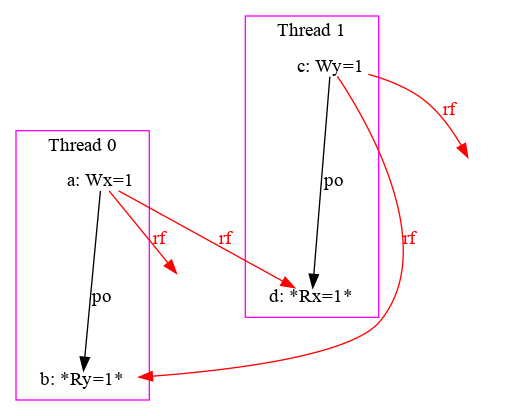
\includegraphics[width=1.2\linewidth]{img/my/sb-example/SB-dot.png}
  \caption{Final state: \texttt{(0:EAX=1,~1:EAX=1)}}
  \label{simple_wmm_x86_pic:sub1}
\end{subfigure}
\hfill
\begin{subfigure}[t]{.23\textwidth}
  \centering
  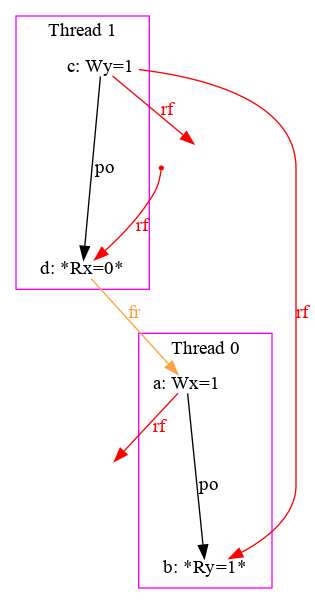
\includegraphics[width=.9\linewidth]{img/my/sb-example/SB-dot-2.png}
  \caption{Final state: \texttt{(0:EAX=1,~1:EAX=0)}}
  \label{simple_wmm_x86_pic:sub2}
\end{subfigure}
\hfill
\begin{subfigure}[t]{.23\textwidth}
  \centering
  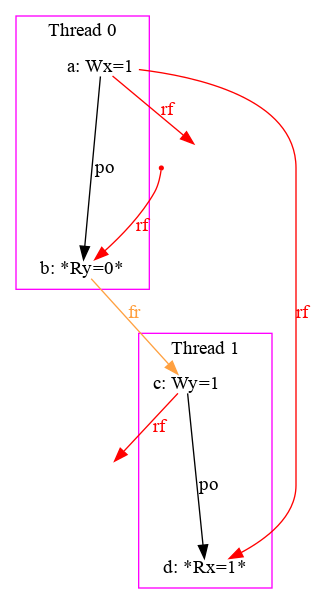
\includegraphics[width=.9\linewidth]{img/my/sb-example/SB-dot-3.png}
  \caption{Final state: \texttt{(0:EAX=1,~1:EAX=1)}}
  \label{simple_wmm_x86_pic:sub3}
\end{subfigure}
\hfill
\begin{subfigure}[t]{.23\textwidth}
  \centering
  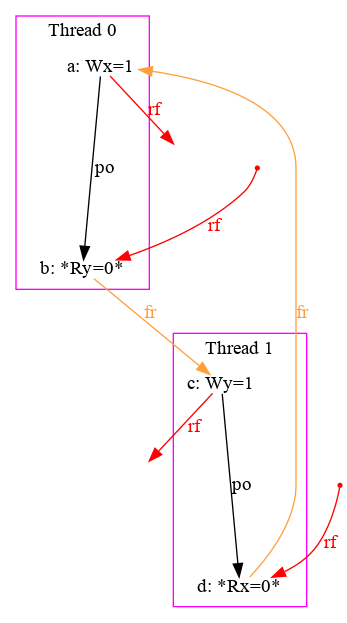
\includegraphics[width=.9\linewidth]{img/my/sb-example/SB-dot-4.png}
  \caption{Final state: \texttt{(0:EAX=0,~1:EAX=0)}}
  \label{simple_wmm_x86_pic:sub4}
\end{subfigure}
\hfill
\caption{Possible candidate executions for the litmus test Example~\ref{simple_wmm_x86}}
\label{simple_wmm_x86_pic}
\end{figure}

Thus, there are only four possible executions defined by the choice of \rf-relation.
The candidate executions pictured in Figures~\ref{simple_wmm_x86_pic:sub1}--\ref{simple_wmm_x86_pic:sub3} are consistent both under strong memory model SC and under relaxed memory models x86-TSO, Power, ARM, and some others.
However, the execution shown in Figure~\ref{simple_wmm_x86_pic:sub3} is still consistent under relaxed-memory architectures, but it becomes inconsistent under SC architecture as it forbids cycles over~$\fr\cup\po$.
%However, the Power memory model allows such cycles, therefore %TODO: include load buffering example, see presentation pdf


\section{\cat{} language}
\label{ch:wmm:cat}

Weak memory models are defined via \cat{} language~\cite{alglave2016syntax}.
This is a domain specific language for describing consistency properties of concurrent programs.
The language combines expressive power of a functional language (it is inspired by OCaml and adopts its types, first-class functions, pattern matching and other features) with types, operations and assertions that are specific for operating with relations and executions.
%represents the functional language extended by the theory of  allows to axiomatically define derived relations, architecture-specific fences, and constraints over relations.
In \cat{}, new relations can be defined via the keyword \texttt{let} and the following operators over relations~\cite{alglave2016syntax}. % 3.1.6 Relations between events

%TODO: this is binary relations. ADD UNARY RELS!

Below we enumerate pre-defined operators over relations and sets of events:

\begin{enumerate}
  \item \textit{Unary operations}:
    \begin{itemize}
      \item \textit{the complement} of a relation \rel{r} is $\rel{\textasciitilde r}$,
      \item \textit{the transitive closure} of a relation \rel{r} is $\rel{r+}$,
      \item \textit{the reflexive closure} of a relation \rel{r} is $\rel{r?}$,
      \item \textit{the reflexive-transitive closure} of a relation \rel{r} is $\rel{r*}$, and
      \item \textit{the inverse} of a relation \rel{r} is $\invrel{r}$.
    \end{itemize}
  \item \textit{Binary operations:}
  \begin{itemize}
    \item \textit{the union} of two relations \rel{r1} and \rel{r2} is \rel{r1\,|\,r2},
    \item \textit{the intersection} of two relations \rel{r1} and \rel{r2} is \rel{r1\,\&\,r2},
      \item \textit{the difference} of two relations \rel{r1} and \rel{r2} is $\mathtt{r1 \relminus r2}$, and
    \item \textit{the sequence} of two relations \rel{r1} and \rel{r2} is \rel{r1;r2}, which is defined as the set of pairs \rel{(x,y)} such that there exists an intervening \rel{z}, such that $\rel{(x,z)} \in \rel{r1}$ and $\rel{(z,y)} \in \rel{r2}$.
  \end{itemize}
\end{enumerate}

For instance, the \fr-relation is defined as a sequence of inverted \rf-relation and \co-relation: $\mathr{fr} = (\mathr{rf}^{-1};\mathr{co})$. As an example memory model definition in \cat{} language, the the x86-TSO can be found in Appendix~\ref{apx:x86cat}. This memory model asserts acyclicity of communication relation, \rel{po-loc} relation, \rel{mfence} relation and some other derived relations~\cite{owens2009better}.

\chapter{Portability analysis as an SMT~problem}
\label{ch:enc}


% TODO: Add intro to the bounded reachability analysis using SAT -- ? 

% TODO: other tools for bounded model-checking: 


%TODO: the method used by Porthos is complete and efficient, but the implementation sucks. Why? 1), 2), 3). How can it be fixed? 1), 2), 3).

%TODO: more about SMT-(= SAT + constraints expressed in background theories. Exapmles of theories that we use and that are implem-ted in Z3).

As it has been discussed in Chapter~\ref{ch:intro}, the program may behave differently when compiled for different parallel hardware architectures.
This may cause the portability bugs, the behaviour that is allowed under one architecture and forbidden under another. 
%already said:
%Although the research of weak memory models has achieved considerable success, most works remain to be rather theoretical that practical and serve mostly as tools for better understanding the concurrent nature of programs.
% The first tool that tackles the problem 
%The first work that has investigated the practical approach of modelling and verification the real-world programs with respect to weak memory models was ~\cite{Porthos17a}  
In this Chapter, we describe the general task of analysing the concurrent software portability
%may be stated 
as a \textit{bounded reachability} problem, which in turn can be reduced to a SMT problem~\cite{Porthos17a}.

%TODO: sound, complete...

\section{Model checking and reachability analysis}
\label{ch:enc:mc}

The model checking is the problem of verifying the system (the model) against a set of constraints (the specification)~\cite{dkw2008}.
As the state machine model is the most widespread mathematical model of computation, most classical model checking algorithms explore the state space of a system in order to find states that violate the specification.

The general scheme of model checking is the following. 
The analysing system (the \textit{model}) is represented as a transition system, a directed graph with labelled nodes representing states of the system.
Each state corresponds to the unique subset of atomic propositions that characterise its behavioural properties.
Once the model has been constructed, it can be checked for compliance to the \textit{specification}.

Usually, the specification defines temporal constraints over the properties of the system.
For instance, the specification assert may state that the property \textit{always} holds (the \textit{safety}) or the property will \textit{eventually} hold (the \textit{liveness}).
Commonly, the \textit{Linear Temporal Logic~(LTL)} or \textit{Computational Tree Logic~(CTL)} (along with their extensions) is used as a specification language due to the expressiveness and verifiability of their statements.

In the described scheme, the model checking problem is reducible to the reachability analysis, an iterative process of a systematic exhaustive search in the state space.
This approach is called \textit{Unbounded Model Checking~(UMC)}.
However, all model checking techniques are exposed to the \textit{state explosion problem} as the size of the state space grows exponentially with respect to the number of state variables used by the system (its size).
In case of modelling concurrent systems, this problem becomes much more considerable due to exponential number of possible interleavings of states.
Therefore, the research in model checking over past 40 years was fighting the state explosion problem mostly by optimising search space, search strategy or basic data structures of existing algorithms.

One of the first techniques that optimises the search space considerably is the symbolic model checking with \textit{Binary Decision Diagrams~(BDDs)}.
Instead of processing each state individually, in this approach the set of states is represented by the BDD, a data structure that allow to perform operations on large boolean formulas efficiently~\cite{clarke2012model}.
The BDD representation can be linear of size of variables it encodes if the ordering of variables is optimal, otherwise the size of BDD is exponential.
The problem of finding such an optimal ordering is known as NP-complete problem, which makes this approach inapplicable in some cases.

The other idea is to use satisfiability solvers for symbolic exploration of state space~\cite{clarke2001bounded}.
In this approach, the state space exploration consists of the sequence of queries to the SAT-solver, represented as boolean formulas that encode the constraints of the model and the finite path to a state in the corresponding transition system.  
%This approach uses an iterative process of constructing queries to the SAT-solver as a boolean formula which encodes the constraints of the model and the finite path to a state in the corresponding transition system. 
%Due to the SAT-solver.
This technique is called \textit{bounded model checking (BMC)} as the search process is being repeated up to the user-defined bound $k$, which may result to incomplete analysis in general case.
However, there exist numerous techniques for making BMC complete for finite-state systems~(e.g.,~\cite{shtrichman2000tuning}).
%As well as the BMC problem, the approach used by \porthos{}

%For instance, the idea of grouping states with similar properties into equivalence classes lead to the concept of traces in concurrent systems proposed by A.~Mazurkiewicz in 1986~\cite{mazurkiewicz1986trace}. 


\section{Portability analysis as a bounded reachability problem}
\label{ch:enc:enc}

%TODO: overapproximation. loops, Rice's thm. Within the bound, the method is complete.

In general, a BMC problem aims to examine the non-reachability of the "undesirable" states of a finite-state system.
Let $\vec{x} = (x_1, x_2, ..., x_n)$ be a vector of $n$ variables that uniquely distinguishes states of the system; let $\textit{Init}(\vec{x})$ be an \textit{initial-state predicate} that defines the set of initial states of the system; let $\textit{Trans}(\vec{x}, \pvec{x}')$ be a \textit{transition predicate} that signifies whether there the transition from state $\vec{x}$ to state $\pvec{x}'$ is valid; let $\textit{Bad}(\vec{x})$ be a \textit{bad-state predicate} that defines the set of undesirable states.
Then, the BMC problem, stated as the reachability of the undesirable state withing $k$ steps, is formulated as following:
%\begin{equation}
$\texttt{SAT}( \textit{Init}(\vec{x_0}) \land \textit{Trans}(\vec{x}_0, \vec{x}_1) \land ... \land \textit{Trans}(\vec{x}_{k-1}, \vec{x}_k) \land \textit{Bad}(\vec{x}_k) )$.
%\end{equation}

The portability analysis problem may also be stated as a reachability problem, where the undesirable state is one reachable under the target~$\mathcal{M_T}$ memory model and unreachable under the source memory model~$\mathcal{M_S}$.
%However, unlikely a BMC problem, the portability analysis does not require to call the SMT solver repeatedly, since (imperative) programs may be converted as acyclic state graph (by reducing the loops, see Section~\ref{ch:impl:proc:x-transf}) and the $Trans$ predicate may be stated only for the final state of a program.
Consider the function $\textit{cons}_{\mathcal{M}}(P)$ calculates the set of executions of program $P$ consistent under the memory model $\mathcal{M}$. Then, the program $P$ is called portable from the source architecture (memory model) $\mathcal{M_S}$ to the target architecture $\mathcal{M_T}$ if all executions consistent under $\mathcal{M_T}$ are consistent under $\mathcal{M_S}$~\cite{Porthos17a}:

\begin{definition}[Portability]
Let $\mathcal{M_S}$, $\mathcal{M_T}$ be two weak memory models. A program $P$ is portable from $\mathcal{M_S}$ to $\mathcal{M_T}$ if 
$\textit{cons}_{\mathcal{M_T}}(P) \subseteq \textit{cons}_{\mathcal{M_S}}(P)$
\end{definition}

Note that the definition of portability requirements against \textit{executions} is strong enough, as it implies the portability against \textit{states} (the \textit{state-portability})~\cite{Porthos17b}.
The result SMT-formula $\phi$ that encodes the portability problem should contain both encodings of control-flow $\phi_{CF}$ and data-flow $\phi_{DF}$ of the program, and assertions of both memory models: ${\phi \defeq \phi_{CF} \land \phi_{DF} \land \phi_{\mathcal{M_T}} \land \phi_{\lnot\mathcal{M_S}}}$. If the formula is satisfiable, there exist a portability bug.
%The control-flow and data-flow encodings are standard for BMC~\cite{collavizza2006exploration}, they are described below. 
%However, encoding of memory models requires additional techniques due to recursive definitions of relations, that were proposed in~\cite{Porthos17a}.


\subsection{Encoding for the control-flow} %Encoding the control-flow constraints}
\label{ch:enc:enc:cf}

The control-flow of a program is represented by the \textit{control-flow graph}, a directed acyclic connected graph with a single source and multiple sink nodes. %TODO: footnote why multiple sinks
In a control-flow graph, there are two types of edges (transitions): \textit{primary transitions} that denote unconditional jumps or if-true-transitions (pictured with solid lines), and \textit{alternative transitions} that denote if-false-transitions (pictured with dotted lines).
Each node on graph can have either one successor (primary) or two successors (both primary and alternative); only computation events can serve as a branching point).
However, each merge node can have any positive number of predecessors, where each edge may be either primary or alternative.

While working on \porthos[2], we have applied some modifications to the encoding scheme for the control-flow.
The changes are conditioned by the need to be able to process an arbitrary control-flow produced by conditional and unconditional jumps of the C language.
For that, we compile the \textit{Abstract Syntax Tree~(AST)} of the parsed C-code to the plain event-flow graph.
We show %TODO! to show, actually!!!
that the new encoding is smaller than the old one used in \porthos{} since it does not produces new variables for each high-level statement of the input language.
%The \tool{PORTHOS} tool encodes the \textit{instructions}, which have recursive nature, in a recursive manner. This means, it adds synthetic composite instructions for both linear (sequential) and non-linear (branching) instructions. 
For instance, \porthos{} used the encoding scheme where the control-flow of the sequential instruction $i_1 = i_2; i_3$ was encoded as
$\phi_{CF}(i_2;i_3) \defeq (cf_{i_1} \Leftrightarrow (cf_{i_2} \land cf_{i_3})) \land \phi_{CF}(i_2) \land \phi_{CF}(i_3)$,
and control-flow of the branching instruction $i_1 = (c\,?\,i_2\!:\!i_3)$ was encoded as
$\phi_{CF}(c\,?\,i_2\!:\!i_3) \defeq (\textit{cf}_{i_1} \Leftrightarrow (\textit{cf}_{i_2} \lor \textit{cf}_{i_3})) \land \phi_{CF}(i_2) \land \phi_{CF}(i_3)$
(here we used the notation of C-like ternary operator `\texttt{x?y:z}' for defining the conditional expression `$\texttt{if}\;x\;\texttt{then}\;y\;\texttt{else}\;z$').
In contrast, the new scheme implemented in \porthos[2] firstly compiles the recursive high-level code into the linear low-level event-based representation, that is then encoded into an SMT-formula. The encoding of branching nodes depends on the \textit{guards}, the value of conditional variable on the branching state, which in turn is encoded as data-flow constraint (see Section~\ref{ch:enc:enc:df}).

All control-flow edges contain a label that denotes the \textit{guard}, a predicate that determines the transition.
An empty guard (a \textit{true} predicate) is denoted as $\epsilon$.
A guard depends on the data-flow of the program, it represents a memory unit or a computational expression that is liable to the weak memory model relaxations.
The branching expressions that support more than two outgoing control-flow edges may be useful for describing non-deterministic transition systems, where the guards are not necessarily mutually exclusive.
However, as the C language supports only binary logic (\textit{if-then-else} branching), \porthos[2] builds only two possible outcomes of evaluating a guard (\textit{primary} and \textit{alternative} transition).


\begin{figure}%[b]
  \centering
  \begin{minipage}{\textwidth}
      \begin{subfigure}[b]{0.3\textwidth}
        \makebox[\textwidth]{
        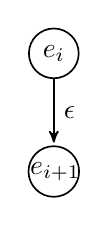
\begin{tikzpicture}[->,>=stealth',shorten >=1pt,auto,node distance=1.5cm,semithick]
            \node[c] (1) [] {$e_i$};
            \node[c] (2) [below of=1] {$e_{i+1}$};
            \path[->]
            (1) edge [] node {$\epsilon$} (2)
            ;
        \end{tikzpicture}
        }
        \caption{Sequence of events (seq)}
        \label{encode:cf:seq}
    \end{subfigure}
    ~
    \begin{subfigure}[b]{0.35\textwidth}
        \makebox[\textwidth] {
        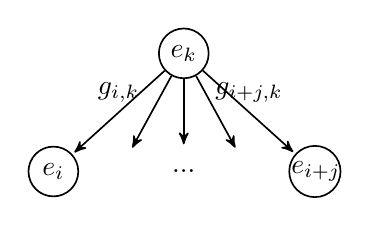
\begin{tikzpicture}[->,>=stealth',shorten >=1pt,auto,node distance=1.5cm,semithick]
            \node[c]           (k)   [] {$e_k$};
            \node[c,draw=none] (iii) [below of=k] {$...$};
            \node[c,draw=none] (ii)  [left=0.2cm of iii] {};
            \node[c]           (i)   [left=0.2cm of ii] {$e_i$};
            \node[c,draw=none] (iv)  [right=0.2cm of iii] {};
            \node[c]           (v)   [right=0.2cm of iv] {$e_{i+j}$};
            \path[->]
            (k) edge [above] node {$g_{i,k}$} (i)
            (k) edge [] node {} (ii)
            (k) edge [] node {} (iii)
            (k) edge [] node {} (iv)
            (k) edge [above] node {$g_{i+j,k}$} (v)
            ;
        \end{tikzpicture}
        }
        \caption{Conditional branching (br)}
        \label{encode:cf:br}
    \end{subfigure}
    ~
    \begin{subfigure}[b]{0.25\textwidth}
        \makebox[\textwidth]{
        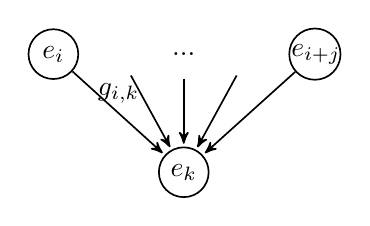
\begin{tikzpicture}[->,>=stealth',shorten >=1pt,auto,node distance=1.5cm,semithick]
            \node[c] (i) [] {$e_i$};
            \node[c,draw=none] (ii) [right=0.2cm of i] {};
            \node[c,draw=none] (iii) [right=0.2cm of ii] {$...$};
            \node[c,draw=none] (iv) [right=0.2cm of iii] {};
            \node[c] (v) [right=0.2cm of iv] {$e_{i+j}$};
            \node[c] (k) [below of=iii] {$e_k$};
            \path[->]
            (i) edge [above] node {$g_{i,k}$} (k)
            (ii) edge [above] node {} (k)
            (iii) edge [] node {} (k)
            (iv) edge [] node {} (k)
            (v) edge [] node {} (k) %sloped
            ;
        \end{tikzpicture}
        }
        \caption{Branch merging (mer)}
        \label{encode:cf:merge}
    \end{subfigure}
    %
    \caption{Possible mutual arrangements of events in a control-flow graph} %Linear and non-linear cases of a control-flow graph}
    \label{encode:cf}
\end{minipage}
\end{figure}

Let $\fx:\,\mathbb{E}\,\rightarrow\,\{0,1\}$ be the predicate that signifies the fact that the event has been e\textbf{x}ecuted (and, consequently, has changed the state of the system).
%Let $\fv:\,\mathbb{C}\,\rightarrow\,\mathbb{R}$ be the function that returns the value of the computation event (evaluates it) that will be computed once the event is executed (strictly speaking, it returns the \textit{set} of values determined by the \rf-relation; see Section~\ref{ch:wmm:model:relations} for details on relations).
%We distinguish the function ${\fv_g\;:\;\mathbb{C}_g\;\rightarrow\;\{0,1\}}$ that evaluates the guard computation event. In the result formula, all symbols $\fx(e_i)$ and $\fv(e_i)$ are encoded as boolean variables.
Consider the possible mutual arrangements of nodes in a control-flow graph presented in Figure~\ref{encode:cf}.

\begin{align}
\phi_{CF_{seq}} \defeq \quad & \fx(e_{i+1}) \Rightarrow \fx(e_i) \label{enc:cf:seq} \\
\phi_{CF_{br}}  \defeq \quad & [\fx(e_i) \Rightarrow \fx(e_k)] \ \land \ \cdots \ \land \ [\fx(e_{i+j}) \Rightarrow \fx(e_k)] \nonumber \\
                       \land & \ [\fx(e_i) \land \fx(e_k) \Rightarrow g_{i,k}] \ \land \ \cdots \ \land \ [\fx(e_{i+j}) \land \fx(e_k) \Rightarrow g_{i+j,k}] \nonumber \\
                       \land & \ \cdots \nonumber \\
                       \land & \ ( \bigvee_{e_l \in \ \texttt{succ}(e_m)} \ \
                               \bigvee_{\begin{subarray}{l}e_n \in \ \texttt{succ}(e_k) \\ e_n \neq e_m\end{subarray}} 
                              \! \lnot [\fx(e_m) \land \fx(e_n)] \ ) \label{enc:cf:br} \\
\phi_{CF_{mer}} \defeq \quad & \fx(e_k) \Rightarrow (\bigvee\limits_{e_p \in \ \texttt{pred}(e_k)}^{} \fx(e_p)) \label{enc:cf:merge}
\end{align}

For these cases, we propose the encoding scheme that uniquely encodes each node of graph and at the same time allows to encode partially executed program.
%TODO: say about epsilon on (c) picture
Equation~\ref{enc:cf:seq} shows the encoding for the sequential control-flow represented in Figure~\ref{encode:cf:seq} and reflects the fact that the event $e_2$ can be executed iff the event $e_1$ has been executed.
Equation~\ref{enc:cf:br} shows the encoding for the branching control-flow depicted in Figure~\ref{encode:cf:br}, that considers both transitions and guards.
Also, adding negations of pairwise conjunctions over all successors of the branching node, the encoding forbids the execution of two branches simultaneously.
Equation~\ref{enc:cf:merge} shows the encoding for the control-flow of a merge-point represented in Figure~\ref{encode:cf:merge}: the event $e_k$ is executed if either of its predecessors has been executed, regardless the type of the transition.
Note that the sequential control-flow is a special case of branching with the only transition guard $\epsilon$ (that is encoded as \texttt{true}).
%TODO: maybe add the overall formula \phi_{CF} ?

For sake of correctness of the encoding, we require all branches to have at least one event.
Thus, for branching statements that do not have any events in one of the branches (such a branch represents a conditional jump forward), we add the synthetic \textit{nop-event} as it is shown in Figure~\ref{encode:branching:nop}.

\begin{figure}%[!h]
    \centering
    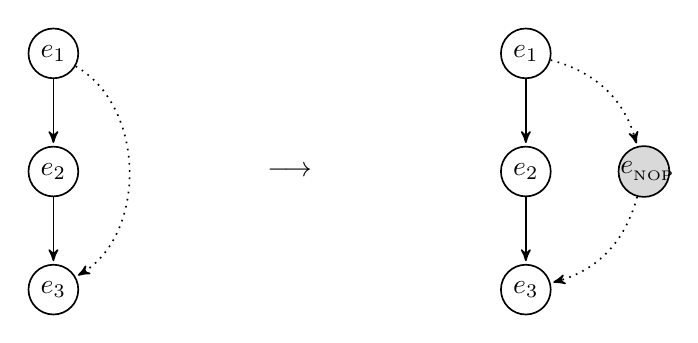
\begin{tikzpicture}[->,>=stealth',shorten >=1pt,auto,node distance=1.5cm,semithick]
        \node[c] at (0,0) (1a) {$e_1$};
        \node[c] at (0,-1.5) (2a) {$e_2$};
        \node[c] at (0,-3) (3a) {$e_3$};
        \node[c,draw=none] at (3,-1.5) (arr) {$\longrightarrow$};
        \node[c] at (6,0) (1b) {$e_1$};
        \node[c] at (6,-1.5) (2b) {$e_2$};
        \node[c,fill=black!15] at (7.5,-1.5) (nop) {$e_{_{\mbox{\tiny NOP}}}$};
        \node[c] at (6,-3) (3b) {$e_3$};
        \path[->]
        (1a) edge [] node {} (2a)
        (2a) edge [] node {} (3a)
        (1a) edge [dotted,bend left=60] node {} (3a)
        (1b) edge [] node {} (2b)
        (2b) edge [] node {} (3b)
        (1b) edge [dotted,bend left] node {} (nop)
        (nop) edge [dotted,bend left] node {} (3b)
        ;
    \end{tikzpicture}
    \caption{Transformation of the forward-jump control-flow}
    \label{encode:branching:nop}
\end{figure}

As an example of the control-flow encoding, consider the event-flow graph in Figure~\ref{fig:graph-example}, which has two branching points and one merge point with three incoming transitions.
To illustrate the correctness of the encoding, consider the path $e_1 \rightarrow e_2 \rightarrow e_4$.
This means, in the formula $\phi_{CF}$, the variables $\fx(e_1)$, $\fx(e_2)$ and $\fx(e_4)$ will have the value $1$, and the variable $\fx(e_3)$ will be assigned to $0$.
It is easy to check that the $\phi_{CF}$ is satisfiable by the chosen SMT-model (considering the guards $g_{1,2}$ and $g_{2,4}$ that define this path to be evaluated to $1$).

Next, consider the path $e_1 \rightarrow e_3 \rightarrow e_4$, which is not allowed by the control-flow graph.
The corresponding model $\fx(e_1)=1$, $\fx(e_2)=0$, $\fx(e_3)=1$ and $\fx(e_4)=1$ does not satisfy the formula $\phi_{CF}$.
The proposed encoding for the control-flow works not only for the whole graph: it can be used for encoding partial control-flow graph.
For example, the model $\fx(e_1)=1$, $\fx(e_2)=1$, $\fx(e_3)=0$ and $\fx(e_4)=0$, which encodes the path $e_1 \rightarrow e_2$, satisfies $\phi_{CF}$.

\begin{figure}
\begin{minipage}{.4\textwidth}
\centering
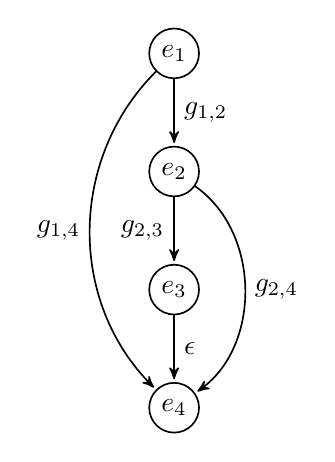
\begin{tikzpicture}[->,>=stealth',shorten >=1pt,auto,node distance=1.5cm,semithick]
    \node[c] (i)   [] {$e_1$};
    \node[c] (ii)  [below of=i] {$e_2$};
    \node[c] (iii) [below of=ii] {$e_3$};
    \node[c] (iv)  [below of=iii] {$e_4$};
    \path[->]
    (i) edge [right] node {$g_{1,2}$} (ii)
    (ii) edge [left] node {$g_{2,3}$} (iii)
    (iii) edge [right] node {$\epsilon$} (iv)
    (i) edge [left,bend right=45] node {$g_{1,4}$} (iv)
    (ii) edge [right,bend left=55] node {$g_{2,4}$} (iv) %sloped
    ;
\end{tikzpicture}
\end{minipage}
%
\begin{minipage}{.6\textwidth}
\centering
\begin{align*}
\phi_{CF} \defeq \ & [\fx(e_2) \Rightarrow \fx(e_1)] \\
                 \ & \land [\fx(e_3) \Rightarrow \fx(e_2)] \\
                 \ & \land [\fx(e_4) \Rightarrow (\fx(e_1) \lor \fx(e_2) \lor \fx(e_3))] \\
                 \ & \land [\fx(e_1) \land \fx(e_2) \Rightarrow g_{1,2}] \\
                 \ & \land [\fx(e_1) \land \fx(e_4) \Rightarrow g_{1,4}] \\
                 \ & \land [\fx(e_2) \land \fx(e_3) \Rightarrow g_{2,3}] \\
                 \ & \land [\fx(e_2) \land \fx(e_4) \Rightarrow g_{2,4}] \\
                 \ & \land \lnot [\fx(e_2) \land \fx(e_4)] \\
                 \ & \land \lnot [\fx(e_3) \land \fx(e_4)]
\end{align*}
\end{minipage}
\caption{Example of encoding for the control-flow of the event-flow graph}
\label{fig:graph-example}
\end{figure}


\subsection{Encoding for the data-flow}
\label{ch:enc:enc:df}

To encode the data-flow constraints, we use the \textit{Static Single-Assignment~(SSA) form} in order to be able to capture an arbitrary data-flow into a single SMT-formula.
The SSA form requires each variable to be assigned only once within entire program.
In contrast, \porthos{} used the \textit{Dynamic Single-Assignment~(DSA)} form, that requires indices to be unique within a branch.
Although the number of variable references (each of which is encoded as unique SMT-variable) on average is logarithmically less in the case of the DSA form than the SSA form, the result SMT-formula still needs to be complemented by same number of equality assertions when encoding the data-flow of merge points~\cite{Porthos17a}.

Following~\cite{Porthos17b}, the indexed references of variables are computed in accordance with the following rules:
%\begin{enumerate}[noitemsep,topsep=0pt]
(1)~any access to a shared variable (both read and write) increments its SSA-index;
(2)~only writes to a local variable increment its SSA-index (reads preserve indices);
(3)~no access to a constant variable or computed (evaluated) expression changes their %SSA-index.
%\end{enumerate}
These rules determine the following encoding of load, store and computation events within single thread:
%TODO: maybe add the overall formula \phi_{DF} ?
%
\begin{align}
    \phi_{DF_{e = \texttt{load}(r \leftarrow l)}}  \defeq \ & [\fx(e) \Rightarrow (r_{i+1} = l_{i+1})] \\
    \phi_{DF_{e = \texttt{store}(l \leftarrow r)}} \defeq \ & [\fx(e) \Rightarrow (l_{i+1} = r_i)] \\
    \phi_{DF_{e = \texttt{eval}(\cdot)}}           \defeq \ & [\fx(e) \Rightarrow \fv(e)] % \\
\end{align}

To convert the program into SSA form, for each event each variable that is declared so far (either local or shared) is mapped to its indexed reference; this information is stored in the SSA-map "event \textit{to} variable \textit{to} SSA-index". %for each event stores the map that each declared variable maps to its SSA-index
%"$\{$ event : $\{$ variable : index $\}\}$",
%"$\left\{$ event : $\left\{$ variable : index $\right\} \right\}$",
The SSA-map is computed iteratively while traversing the event-flow graph in topological order as it is described in Algorithm~\ref{algorithm:ssa-map}.

\begin{algorithm}
    \caption{Algorithm for computing the SSA-indices}\label{alg:compute-ssa}
    \algorithmicrequire{The event-flow graph $G = \langle N, E \rangle$ where $V$ is the set of nodes (events), $E$ is the set of control-flow transitions, $e_0$ is the entry node}
    \algorithmicensure{The SSA-map of the form "$\{$ event : $\{$ variable : index $\}\}$"}
    \begin{algorithmic}[1]
        \Function{Compute-SSA-Map}{G}
            \State {$S \gets$ empty map; $S[e_0] \gets$ empty map}
            \ForAll {event $e_i \in G.N$ in topological order}
                \ForAll {predecessor $e_j \in \texttt{pred}(e_i)$}
                    \State {$S[e_i] \gets \texttt{copy}(S[e_j])$}
                    \ForAll {variable $v_k \in$ set of variables accessed by $e_i$ }
                        \State {$S[e_i][v_k] \gets \texttt{max}(S[e_i][v_k], \ S[e_j][v_k])$}
                        \If {need to update the index of $v_k$} \Comment {cases (1)-(2)}
                            \State {$S[e_i][v_k] \gets S[e_i][v_k] + 1$}
                        \EndIf
                    \EndFor
                \EndFor
            \EndFor
        \EndFunction
    \end{algorithmic}
    \label{algorithm:ssa-map}
\end{algorithm}

The time of described algorithm is linear of the size of event-flow graph since it performs only one graph traverse.
%Notwithstanding the overhead of storing (or, equivalently, computing with %TODO: are you sure that 'with'?
%linear time) the predecessors of each node in order to be able to convert the program into an SSA form, the time of such a transformation reduced %TODO: How much ????
%comparing to the algorithm implemented in \porthos, which recomputed SSA-indices recursively for each instruction. %TODO: PROOF OR REMOVE !  Maybe, some words of copying, merging SSA maps ?

As it has been described before, the \rf-relation links data-flow between events %TODO: another word?
of data-flow stored in equivalence assertions over the SSA-variables. 
%The encoding of the \rf-relation, which links the SSA-variables to the original variables, 
The encoding of this linkage left untouched as it is implemented in \porthos: for each pair of events $e_1$ and $e_2$ linked by the \rf-relation, we add the following constraint:
%
\begin{align}
\phi_{DF_{mem}}(e_1, e_2) \defeq \ & [\texttt{rf}(e_1, e_2) \Rightarrow (l_i = l_j)]
\end{align}

where the variable of location $l$ is mapped to the SSA-variable $l_i$ for event $e_1$, and to the SSA-variable $l_j$ for event $e_2$; and the predicate $\texttt{rf}(e_1, e_2)$ is encoded as a boolean variable, which itself equals $true$ if $e_2$ reads the shared variable that was written in $e_1$.


\subsection{Encoding for the memory model} %Encoding the memory model constraints}
\label{ch:enc:enc:wmm}

The basic scheme for encoding the memory model is proposed in~\cite{Porthos17a}.
The encoding consists of two parts: encoding the \textit{derived relations} and encoding the memory model \textit{assertions}.

In an SMT-formula, the relation $x \relarrow{r} y$ is represented by a boolean variable $r(x, y)$ that indicates whether the relation holds.
The derived relations are encoded by fresh boolean variables according to the following rules~\cite{Porthos17b}:
\begin{itemize}[noitemsep,topsep=0pt]
\item $r_1 \cup r_2(e_1, e_2) \defeq r_1(e_1, e_2) \lor r_2(e_1, e_2)$;
\item $r_1 \cap r_2(e_1, e_2) \defeq r_1(e_1, e_2) \land r_2(e_1, e_2)$;
\item $r_1 \relminus r_2(e_1, e_2) \defeq r_1(e_1, e_2) \land \neg r_2(e_1, e_2)$;
\item $r^{-1}(e_1, e_2) \defeq r(e_2, e_1)$;
\item $r^{*}(e_1, e_2) \defeq r^{+}(e_1, e_2) \lor (e_1 = e_2)$;
\item $r_1;r_2(e_1,e_2) \defeq \bigvee\limits_{e_k \in \mathbb{E}}^{} r_1(e_1,e_k) \land r_2(e_k,e_2)$; \ and
\item $r^{+}(e_1, e_2) \defeq \texttt{tc}_{\left\lceil log|\mathbb{E}| \right\rceil} (e_1, e_2), \ where \vspace{0.25em} \\
\texttt{tc}_{0}(e_1,e_2) \defeq r(e_1,e_2), \ and \\
\texttt{tc}_{i+1}(e_1,e_2) \defeq r(e_1,e_2) \lor (\texttt{tc}_{i}(e_1,e_2);\texttt{tc}_{i}(e_1,e_2))$.
\end{itemize}
\vspace{1em}

Note that \cat{} language allows mutually-recursive definitions of relations (for example, `$\texttt{r}_\texttt{1} = \texttt{r}_\texttt{2} \cup (\texttt{r}_\texttt{1}; \texttt{r}_\texttt{1})$').
The basic idea of using the Kleene fixpoint iteration for encoding such relations was also proposed in~\cite{Porthos17a}: for any pair of events $e_1,e_2 \in \mathbb{E}$ and relation $r \subseteq \mathbb{E} \times \mathbb{E}$, we encode a new integer variable $\Phi_{e_1,e_2}^{r}$ that represents the round of Kleene iteration on which the variable $r(e_1, e_2)$ has been set.
 %is used for guessing the execution 

The memory model can assert acyclicity, irreflexivity of emptiness of a relation or a set of events.
As it has been proposed in~\cite{Porthos17a}, encoding the acyclicity assertion uses numerical variable $\Psi_e \in \mathbb{N}$ for each event $e$ in the relation to be asserted: $\textit{acyclic}(r) \defeq (r(e_1,e_2) \Rightarrow (\Psi_{e_1} < \Psi_{e_2}))$.
The irreflexivity assertion as $\textit{irreflexive}(r) \defeq \bigwedge\limits_{e_k \in \mathbb(E)}^{} \lnot r(e_k,e_k)$.

%The ... \wmodel{}

%Most bounded model-checking problems are solved via computing the fixpoint for the

%The encoding of a weak memory model itself does not depend on the analysing program. The problem here...
%recursive definitions and Kleene iteration

%r 1 ∪r 2 (e 1 , e 2 ) ⇔ r 1 (e 1 , e 2 ) ∨ r 2 (e 1 , e 2 )
%r 1 ∩r 2 (e 1 , e 2 ) ⇔ r 1 (e 1 , e 2 ) ∧ r 2 (e 1 , e 2 )
%r 1 \r 2 (e 1 , e 2 ) ⇔ r W
%r −1 (e 1 , e 2 ) ⇔ r(e 2 , e 1 )
%1 (e 1 , e 2 ) ∧ ¬r 2 (e 1 , e 2 )
%r 1 (e 1 , e 3 ) ∧ r 2 (e 3 , e 2 )
%r ∗ (e 1 , e 2 ) ⇔ r + (e 1 , e 2 ) ∨ (e 1 = e 2 )
%r 1 ;r 2 (e 1 , e 2 ) ⇔
%e 3 ∈E
%r + (e 1 , e 2 ) ⇔ tc ⌈log |E|⌉ (e 1 , e 2 ), where
%tc 0 (e 1 , e 2 ) ⇔ r(e 1 , e 2 ), and
%tc i+1 (e 1 , e 2 ) ⇔ r(e 1 , e 2 ) ∨ (tc i (e 1 , e 2 ); tc i (e 1 , e 2 ))
%
%As it is described in~\cite{Porthos17a}, the is based . . .
%~\cite{Porthos17a}%, Section "Programs and Memory Models", subsection "Encoding Derived Relations"

\chapter{The~\texttt{porthos2}:~implementation}
\label{ch:impl}

The main reason for commencing the work on \porthos[2] was the need for processing real-world C programs, which, at first, requires the input language to be extended.
This implies the support not only for new syntactic structures of C language (such as the \texttt{switch} statement or the postfix increment operator \texttt{i++}), but also for its fundamental concepts and features (such as types, pointer arithmetic or first-order functions), which requires revision of the whole architecture of the tool.
Although far not the entire C language has been supported (that, considering its complexity and numerous pitfalls, goes far beyond current thesis%
\footnote{To ensure that, we have merely to look at existing C compilers, for instance, the open-source \texttt{gcc} compiler, that uses a C parser written in more than 18.5 thousand lines (see \url{https://github.com/gcc-mirror/gcc/blob/master/gcc/c/c-parser.c})}%
), we consider the accomplished work as a step towards this.
%This applies not only to instances that simply constitute the syntactic sugar of C language (such as the \texttt{switch} statement or the prefix increment operator \texttt{++i}), but also to its fundamental concepts and features (such as pointer arithmetic or structures).
%However, the architecture of current version of \porthos{} does not allow to ... as it is ....
% Although and optimisation of the tool so that it is able to process real C programs in perspective.

%In current Chapter we discuss the new architecture of \porthos[2].

% function invocations/calls: inlining with binding
% contexts: for now, no ctxs
% comparing to cprover (https://www.cprover.org/cbmc/doc/manual.pdf, page 45, absatz about 'goto') where "the loop is unwound a given number of times" , we SHOULD have 2 modes of unrolling: 1) number of times, and 2) number of high-level instructions executed
% TODO(code): (https://www.cprover.org/cbmc/doc/manual.pdf, page 45) "The break and continue statements are replaced by equivalent goto statements as described in the ANSI-C standard."

% TODO: arrays: cprover manual page 48


%\section{The architecture of \porthos[1]}
\section{General principles}
\label{ch:impl:principles}

The existing implementation of \porthos[1] does not distinguish the event-based program model from the high-level AST, they both are encoded into single SMT-formula (see classes of package `\texttt{dartagnan.program}' of \porthos tool).
Moreover, the syntax tree was implemented as a mutable data structure, which is being modified at all stages of the program (for instance, see the methods `\texttt{dartagnan.program.Program.compile(...)}' of \porthos{} that recursively compute some properties of the AST and change its state).
We are inclined to consider this architecture as one that is fast to develop, but hard to maintain (since it is difficult to guarantee the correctness of the program) and extend (since adding the support for a new high-level instruction requires changing multiple components of the program, from parser to encoder).
%Moreover, we encounter serious problems when we need to add support for control-flow jumps (as \texttt{continue}, \texttt{break}, \texttt{goto} in C).

% todo: in old porthos the strategy soft: print info about error. new: exception on any detected violation of any invariant

Therefore, while working on the new design of \porthos[2], we decided to clearly separate the high-level intermediate code representation (implemented as a recursive AST structure) from low-level event-based representation (implemented as an event-flow graph).
Such a modular architecture allows to support multiple input languages by parsing them and converting parsed syntax trees to a simplified AST. which, along with all other data-transfer objects (DTO), must be immutable, so that it is possible to guarantee the correctness of the program by controlling its invariants.
The immutability in \porthos[2] is implemented via \texttt{final} fields that are assigned by the immutable-object values (either a primitive type, or another immutable object, or an immutable collection provided by the library Guava by Google%
\footnote{Guava project repository: \url{https://github.com/google/guava/}}%
).

During the development of \porthos[2] we mainly followed the \textit{KISS~principle}, which can be exhaustively described in 17 Unix Rules of Eric Raymond~\cite{raymond2003art}.% which include the rule of modularity, the rule of clarity, transparency, extensibility, etc.
The following list summarises the main rules we followed during the development of \porthos[2]:

\vspace{0.5em}
\begin{enumerate}[nolistsep]
  \item \textit{Robustness:}
    \begin{enumerate}[label*=\arabic*.]
      \item usage of immutable data structures for all DTOs;
      \item interrupting the work on errors;
      \item modular architecture: each module can be tested independently;
      \item usage of software design patterns if necessary;
    \end{enumerate}
  \item \textit{Transparency:}
    \begin{enumerate}[label*=\arabic*.]
      \item following the principles of simplicity and readability;
      \item clear and informative program output;
    \end{enumerate}
  \item \textit{Efficiency:}
    \begin{enumerate}[label*=\arabic*.]%[leftmargin=1.5em]
      \item keeping the trade-off between execution time and memory usage;
    \end{enumerate}
  \item \textit{Extensibility:}
    \begin{enumerate}[label*=\arabic*.]%[leftmargin=1em]
      \item clear modular architecture.
    \end{enumerate}
\end{enumerate}


As \porthos[1], the \porthos[2] uses the open-source SMT solver \texttt{Z3} from Microsoft Research~\cite{de2008z3}. However, unlikely its predecessor, the \porthos[2] has an additional abstraction level \zformula{} (see Section~\ref{ch:impl:model:zformula}) that allow to use any other SMT solver. %TODO: *should* allow?

The programming language choice for \porthos[2] was also made in favour of \textit{java}, firstly, in order to be able to reuse some parts and concepts of \porthos[1] that is written in java, and secondly, because the authors find the object-oriented (OOP) concepts of java suitable for modelling languages.
Although java does not show best results in performance benchmarks (for example, comparing to C++~\cite{hundt2011loop, oaks2014java}), the performance cornerstone of \porthos[2] (as well as any other SMT-based code analyser) is the phase of solving the SMT-formula, which is left to the third-party SMT-solver \textit{Z3}%
\footnote{The Z3 project repository: \url{https://github.com/Z3Prover/z3}} %
invoked from \porthos[2] via java API.
However, considering the perspective of using \porthos[2] as a static analyser for real-world programs, the memory optimisation problem must also be taken into account during both encoding and solving stages.
It is worth noting that, for the reasons of simplicity, the \porthos[2] is not a concurrent program, however, we believe that, due to its modular architecture, it can be easily parallelised on the level of program modules.


\section{Architecture}
\label{ch:impl:arch}

The general architecture scheme of \porthos[2] is presented in Figure~\ref{fig:arch}. On the picture, rectangles denote processing units (marked with gear sign with a number of the component for referencing it).

\begin{figure}%[H]
    \centering
  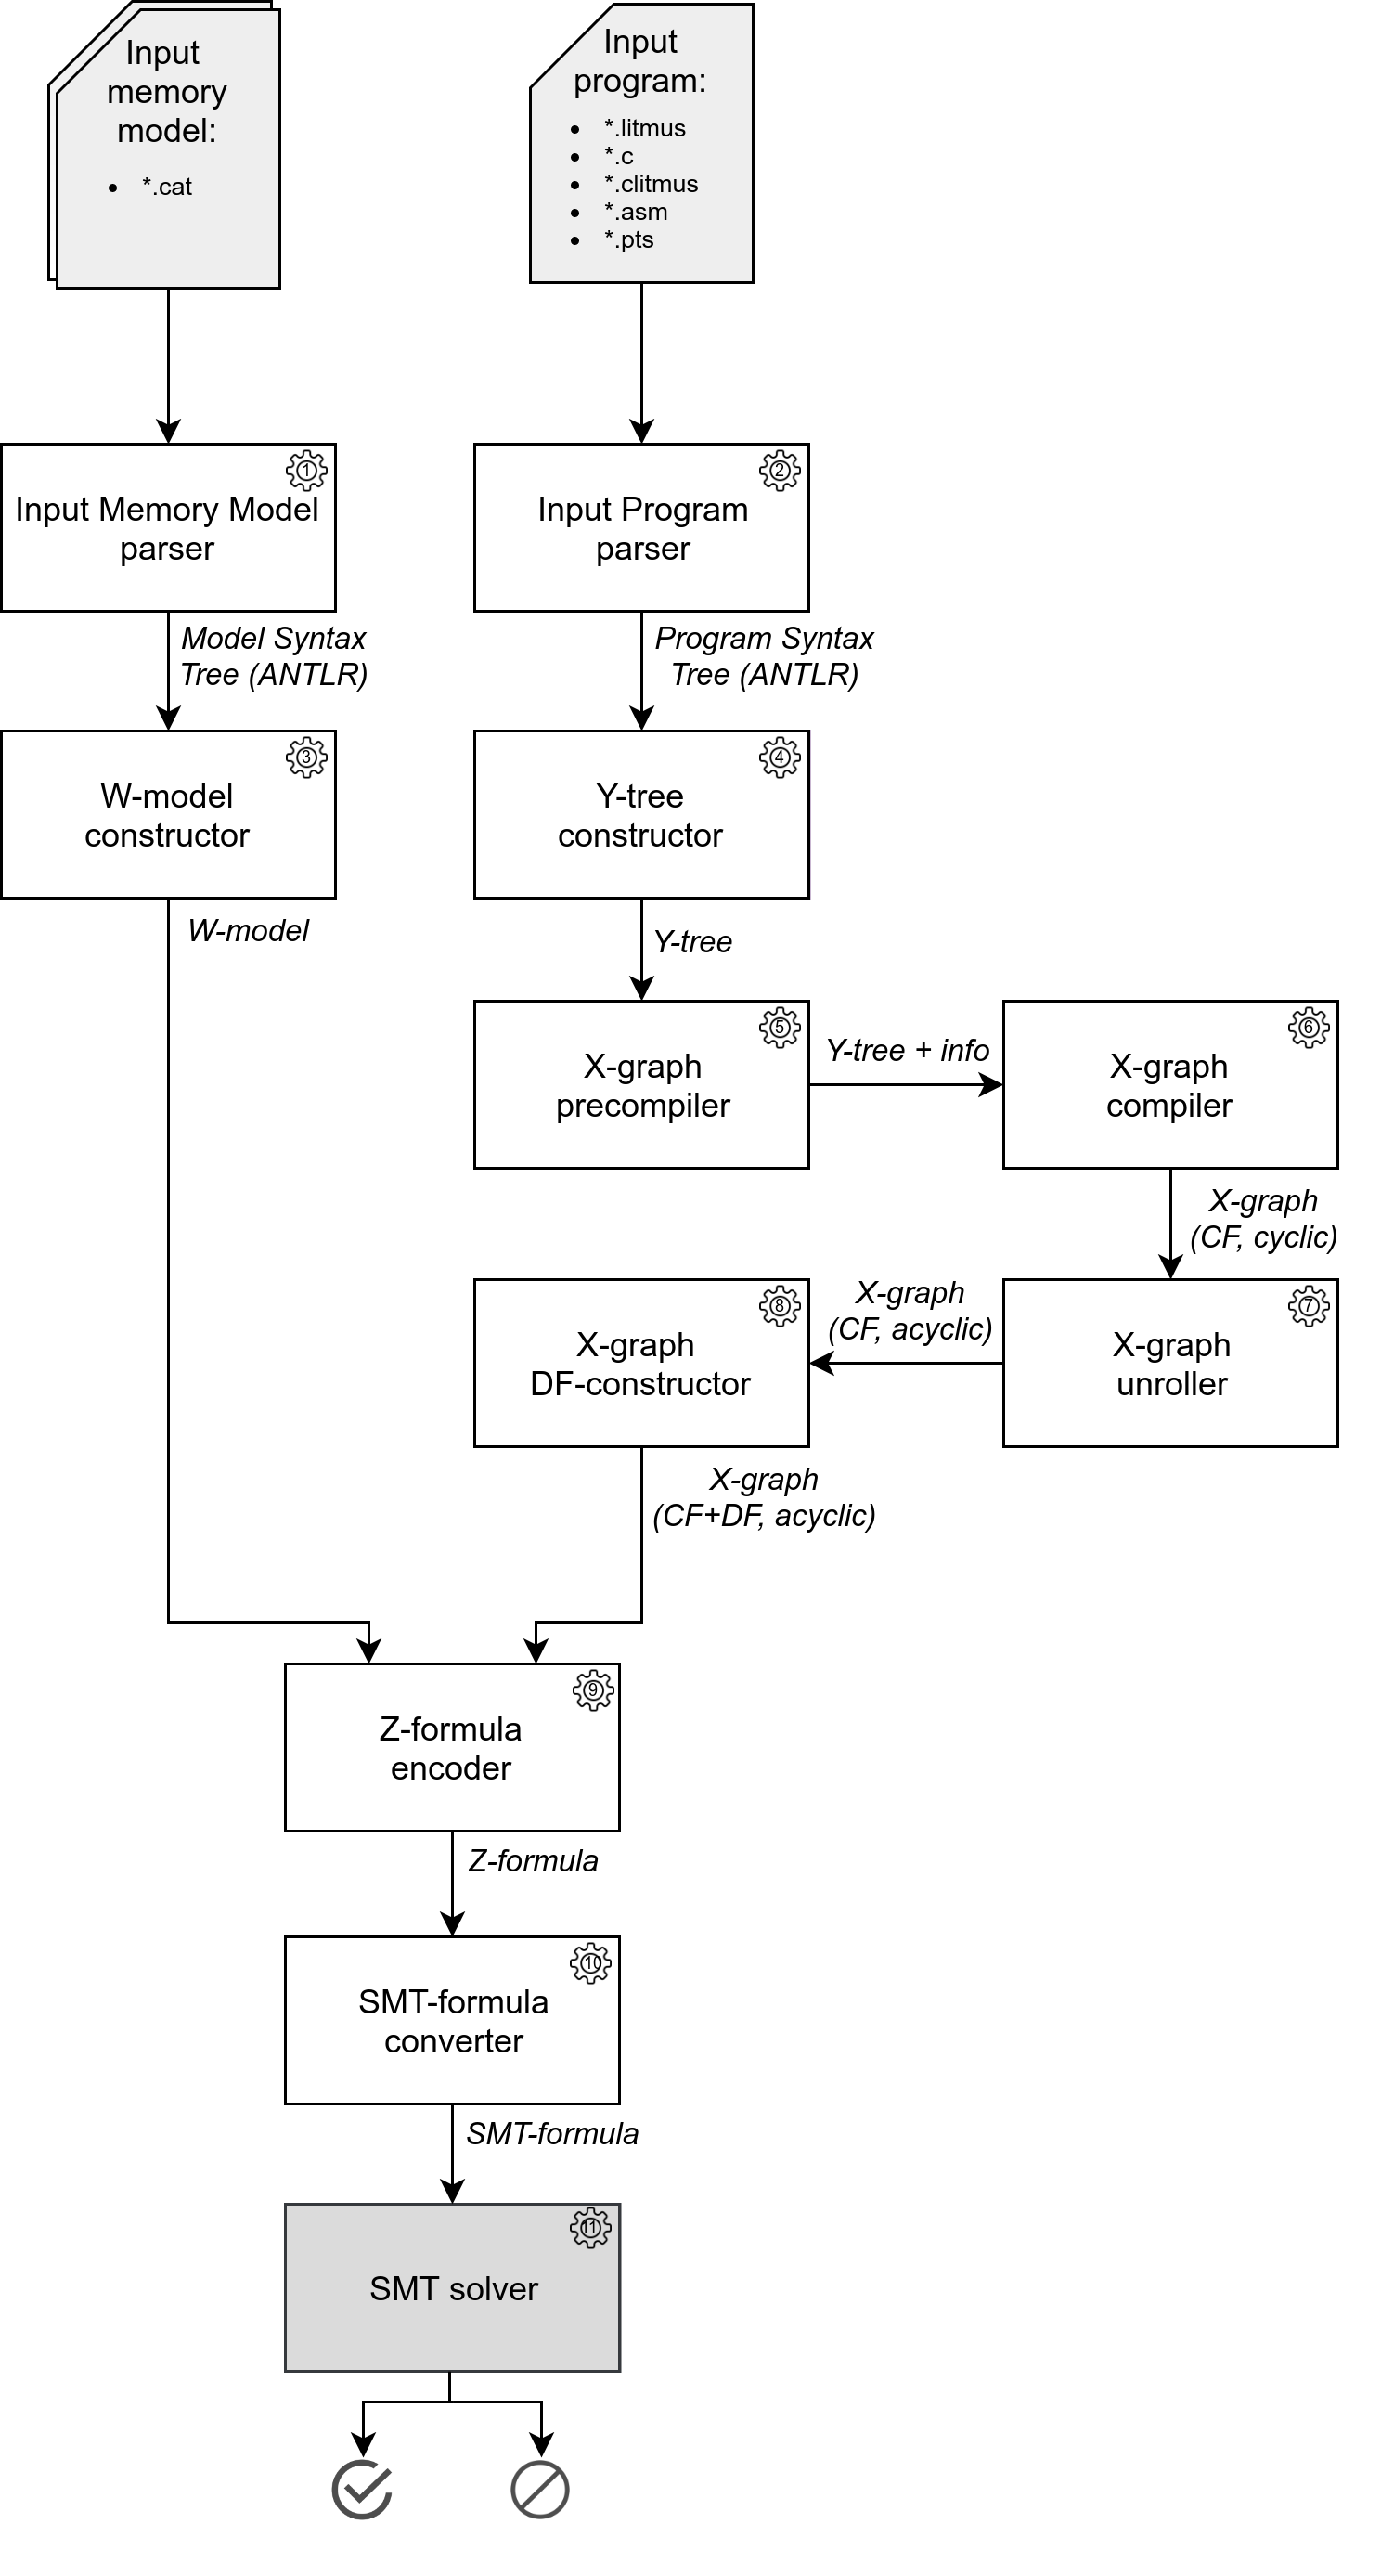
\includegraphics[width=\textwidth,height=\textheight,keepaspectratio]{img/my/draw.io/general_arch.png}
  \caption{The general architecture of \porthos[2]}
  \label{fig:arch}
\end{figure}

The program takes as input the program to be analysed and one (the reachability analysis mode) or two (the portability analysis mode) memory models. The parsed program syntax tree is then converted (Section~\ref{ch:impl:proc:y-constr}) to a program AST called \ytree{}%
\footnote{In order to avoid confusion between different internal representations, we prefix the names of elements of each internal representation with a letter. For instance, we picked the letter `Y' to denote the AST code representation as drawing of this letter resembles the tree branching; with letter `X' we prefix elements of the event-flow graph as the events are to be e\textbf{x}ecuted; and with letter `W' we prefix elements of the \textbf{w}eak memory model AST.} %
(Section~\ref{ch:impl:model:ytree})
%, and the memory model is being parsed (Section~\ref{ch:impl:proc:w-parser}) to another AST called \wmodel{} (Section~\ref{ch:impl:model:wmodel}).
, which then is being pre-processed at the pre-compilation stage (Section~\ref{ch:impl:proc:x-pre-compiler}) in order to collect information necessary for the compilation.
The \ytree{} then is being compiled (Section~\ref{ch:impl:proc:x-compiler}) to an \xgraph{} representation (Section~\ref{ch:impl:model:xgraph}).
The compiled \xgraph{} then undergoes a number of transformations (Section~\ref{ch:impl:proc:x-unroll}) necessary for the encoding into a \zformula{} (Section~\ref{ch:impl:model:zformula}) at the pre-encoding stage (Section~\ref{ch:impl:proc:x-unroll}).
Then, the memory-model constructor (Section~\ref{ch:impl:proc:w-constr}) constructs the derived relations on the basis of the \xgraph{} in order to build the weak memory model \wmodel{} (Section~\ref{ch:impl:model:wmodel}).
Thereafter, \wmodel{} and transformed \xgraph{} are encoded (Section~\ref{ch:impl:proc:z-encoder}) to a \zformula{} representation (a wrapper over an SMT logical formula), which then is passed as an input to the SMT-solver.

\subsection{Program input}
\label{ch:impl:input}
%(for instance, the original input language of \porthos{} tool, two variants of syntax of a litmus test used by \tool{herd}, an assembly language for any supported architecture).

Both \porthos[1] and \porthos[2] use the ANTLR parser generator%
\footnote{The ANTLR project repository: \url{https://github.com/antlr/antlr4}}%
~\cite{parr2013definitive}, a~powerful language processing tool.
The ANTLR takes as input the user-defined grammar of the target language in a BNF-like form and produces the LL(*)-parser and optionally some auxiliary classes (such as listeners and visitors for the syntax tree).
Although this parser may be not as efficient as the hand-written language-optimised parser, it reduces the overhead of implementing the parser significantly.
Among other advantages ANTLR, it is worth of noting that it has rather large collection of officially supported grammars. Nonetheless, the intuitive syntax for defining grammars and numerous of tools for debugging grammars make the ANTLR an attractive instrument for solving the parsing problem.

Figure~\ref{fig:in_grammar_pts} represents the simplified grammar of of input language used by previous version of \porthos{} (the full ANTLR grammar is available at Appendix~\ref{apx:grammar}.

\begin{figure}[h]%[!hb]
\centering
\begin{lstlisting}[mathescape=true,%
                  caption={The sketch of the input language grammar used by \oldporthos},%
                  label={fig:in_grammar_pts},%
                  morekeywords={if,then,else,return,while,program,thread},%
                  breaklines=true,%
                  basicstyle=\ttfamily\scriptsize]
<prog> : <init> <thrd>* <assert>
       ;
<thrd> : thread <tid> <inst>
       ;
<inst> : <atom>
       | <inst> ; <inst>
       | while <pred> <inst>
       | if <pred> { <inst> } <inst>
       ;
<atom> : <reg> <- <expr>
       | <reg> <:- <loc>
       | <loc> := <reg>
       | <reg> = <loc>.load(<atomic>)
       | <loc> = <reg>.store(<atomic>)
       | 'mfence'
       | 'sync'
       | 'lwsync'
       | 'isync'
       ;
<pred> :
       | true
       | false
       | <expr> (and | or) <expr>
       | <expr> ('==' | '!=' | '>' | '>=' | '<' | '>=') <expr>
       ;
<expr> : [0-9]
       | <reg>
       | <expr> ('*' | '+' | '-' | '/' | '%') <expr>
       ;
\end{lstlisting}
\end{figure}

The input language parser used by \porthos[1] suffered from several disadvantages.
Firstly, it contained the parser code inlined into directly the grammar, so that the grammar would serve as a template for the parser code (which is called semantic actions). Such a combining of two rich languages%
\footnote{by the term "reach" we mean "expressiveness": at least, the grammar of the language of semantic actions (i.e., java in our case) is Turing-complete.} %
makes the code hardly understandable, and, therefore, poorly maintainable. In \porthos[2], we clearly separated the parser (generated from the grammar file `\textit{<grammar>.g4}') from the converting the ANTLR syntax tree to the AST, that is one for all  languages of an input program.

Secondly, the semantics of operations was defined syntactically, whereas processing programs written in most modern languages (including C) requires the semantics resolution based on typification%
\footnote{for instance, given two functions
`\lstinline{int foo(int a)}' and `\lstinline{int foo(char a)}', the code `\lstinline{int a = '1'; foo(a);}' will invoke the first method rather than the second one.}.%
As the reader can notice from the grammar sketch in Figure~\ref{fig:in_grammar_pts}, the memory operations of different kinds vary syntactically. For example, the assignment of local computation to a register uses the symbol `\lstinline{<-}', the atomic non-relaxed load operation denoted as `\lstinline{<:-}', non-relaxed store operation denoted as `\lstinline{:=}', and the semantics of relaxed \lstinline{load} and \lstinline{store} are resolved syntactically by matching the method name. In \porthos[2], the semantics of the data-flow operation is determined according to the types of operands, that are determined during the pre-compilation stage (see Section~\ref{ch:impl:proc:x-pre-compiler}). The semantics of the methods also is being resolved during the pre-compilation stage via the \textit{invocation hooks} mechanism (see Section~\ref{ch:impl:proc:x-pre-compiler:hooks}).

Thirdly, the grammar used by \porthos{} had restricted set of allowed operations. For example, it allowed only computations over the local variables, which might lead to inconsistency of the result SMT-formula if the same variable name was used both as a register and as a location, for instance, the in code snippet `\lstinline{x := reg1; reg2 <- (x + 1);}', the first statement interprets the variable \lstinline{x} as a location, while the grammar of second statement requires it to be a register. Also, only integers were processed by the input language parser of \porthos[1]. In \porthos[2], we extended support for primitive types supported by the \texttt{Z3} solver (this apply to 32-bit integers encoded as \texttt{Int}s, floats encoded as \texttt{Real}s, enums encoded as Z3 \texttt{Scalars}).
%TODO : constant arrays? https://rise4fun.com/Z3/tutorial/guide
Thus, adding support for more advanced syntactic structures as pointers, arrays, function definitions and calls was one of the purposes of revising the tool architecture.

The minor drawbacks of grammar used by \porthos[1] include lack of operator associativity (expressions of the form \lstinline{1 + 2 * 3} could not be parsed), incorrectly (in terms of C) implemented grammar rule for the statement (the semicolon punctuator `\lstinline{;}' was implemented as the separator between two statements, whereas in C it serves as a statement terminator). Also, \porthos[1] supports only the litmus-specific syntax for the variables initialisation, however, it allows only ini
tialisation of the shared variable and only by default value \lstinline{0}. The \porthos[2] supports arbitrary declaration to be performed in initialisation statement.


The \porthos[2] uses the C language grammar of proposed in the C11 standard~\cite{jtc2011sc22}, that was extended by litmus test-specific syntax such as initialisation and final-state assertion statements (the original ANTLR grammar can be found in the official repository containing the collection of ANTLR v4 grammars%
\footnote{Repository path: \url{https://github.com/antlr/grammars-v4}}).%
Currently, \porthos[2] can operate only in the intra-procedural analysis mode (analysing single procedure), assuming that each function defined in the input file is being executed in a separate thread.
%TODO: describe more intra- and inter-procedural!
However, the redesigned architecture of \porthos[2] allow to easily support inter-procedural (cross-procedure) analysis by inlining function calls and binding variable contexts.
%TODO: inter: user specifies the repository with code, functions that intended to work in parallel and runs. 
Also, Current version of \porthos[2] simply ignores C processor directives, however, in future it is possible to support it.

%TODO: say sth about 100500 litmus-tests for kernel


\subsection{The internal representations}
\label{ch:impl:model}
%As it has already been mentioned, all internal representations constructed by \porthos[2] are \textit{immutable}.

\subsubsection{Y-tree}
\label{ch:impl:model:ytree}

The first internal representation that \porthos[2] uses is the \ytree{}, which represents a rather high-level AST.
The Apendix~\ref{apx:trees} represents the file tree of main classes that constitute the \ytree{} hierarchy (as the inheritance tree might be obvious for the C-like AST, we confine ourselves to presenting the classes file tree only).

%\columnratio{0.7}%\begin{paracol}{2}
%\switchcolumn%\VerbatimInput{inc/lst/Ytree-tree.out}%\end{paracol}
The abstract syntax tree \ytree{} is an abstraction level suitable for compiling the program to a low-level representation (in case of processing low-level assembly code, it may be directly converted to the \xgraph{} representation).
As the ANTLR syntax tree follows the same structure as the grammar, which is a superset of the real (meaningful) grammar of C language, it lacks multiple concepts of the language (for example, the syntax of indexer access corresponds the grammar rule \lstinline{postfixExpression '[' expression ']'}, that is converted to the \texttt{YIndexerExpression}).
However some details of the syntax might have been abstracted away (for instance, array operations may be emulated by functions invocations, see~\cite[Chapter 5]{gries2012science}), we found this level of abstraction suitable enough for our tasks.

Each \ytree{} element implements the interface \texttt{YEntity} and carries the \texttt{OriginLocation} %
%\textbf{(TODO: Rename CodeLocation->OriginLocation in the code!)} %TODO <--
instance that contains information about the coordinates of the input text that generated the \ytree{} element.

Following the C11 standard~\cite{iso2012iec}, we distinguish a \textit{statement} (\textit{"an action to be performed"}) from an \textit{expression} (\textit{"a sequence of operators and operands that specifies computation of a value, or that designates an object or a function, or that generates side effects, or that performs a combination thereof"}).

All \ytree{} expressions implement the \texttt{YExpression} interface.
On the \ytree{} level, the pointer arithmetic is modelled by the integer number \textit{pointer level} of an expression (although in fact this is the property of a type not of an expression, the y-tree is an untyped syntax tree, therefore the elements \ytree{} should carry this property).
We distinguish the subset of expressions that imply no side-effects, they implement the interface \texttt{YAtom} and can be global or local (which is defined also syntactically).
%\textbf{(TODO:THIS SHOULD BE IN PRE-PROCESSING)} %TODO <--

\vspace{0.5em}
The \ytree{} expressions are the following:

\begin{itemize}%[nolistsep]
  \item \texttt{YBinaryExpression} that model the C binary operator (\textit{relative} operator that compares two expressions of any type, \textit{logical} that processes two boolean expressions, and \textit{numerical} that processes two numerical expressions);
  %\textbf{TODO: rename 'integer'->'numerical' in code} %TODO <--

  \item \texttt{YUnaryExpression} that model the C unary expression (logical negation, numeric prefix and postfix increment and decrement, bitwise complement);

  \item \texttt{YMemberAccessExpression} that has an arbitrary expression of type \texttt{YExpression} as its base expression (it will be resolved during the compilation stage);%TODO: pre-compilation??

  \item \texttt{YIndexerExpression} and \texttt{YInvocationExpression} that as arbitrary expression as its base or arguments (strictly speaking, the indexer expression is an unary-function invocation, but as the SMT solver we use supports the constant-array theory, we can maintain the array type);

  \item \texttt{YAssignmentExpression} that assigns an \texttt{YExpression} to an \texttt{YAtom};

  \item \texttt{YVariableRef} that stores the "reference" to a variable (viz., the name of an object);

  \item \texttt{YLabeledVariableRef} that represents the litmus-specific local variable reference for a certain the process (e.g., `\lstinline{P0:x}' which means the local variable \lstinline{x} of the process \lstinline{P0});

  \item \texttt{YParameter} that represents a typed variable (the type was declared, similarly to the variable definition);

  \item \texttt{YConstant} that represents an untyped non-named constant.
\end{itemize}

%\vspace{0.5em}
Similarly to expressions, all \ytree{} statements implement the \texttt{YStatement} interface. The statements are the following: 
%\textbf{(TODO: extract interface YStatement, create abstract class YStatementBase)} %TODO <--

\begin{itemize}%[nolistsep]
  \item \texttt{YBranchingStatement} representing the \texttt{if-then-else} statement;
  
  \item \texttt{YLoopStatement} representing both \texttt{while}- and \texttt{for}-loops;%TODO:RENAME YWhileLoopStatement->YLoopStatement in code!!!)}
  
  \item \texttt{YJumpStatement} representing unconditional jump (\texttt{goto}-jump to a label and loop-jumps \texttt{break} and \texttt{continue});
  
  \item \texttt{YCompoundStatement} (block statement) representing sequence of \texttt{N} statements grouped into one syntactic unit;
  
  \item \texttt{YLinearStatement} representing a single expression;
  
  \item \texttt{YVariableDeclarationStatement} containing the information about the variable type during the variable declaration.
\end{itemize}

On the \texttt{Y}-level of abstraction, we define the \texttt{YType} as an alias for a type (since the \ytree{} is not typed, all expressions do not have type, however, the \texttt{YType} is used for storing the information of the type for declarations

According to the C standard, \textit{"any statement may be preceded by a prefix that declares an identifier as a label name"}.
The \ytree{} statements of follow this rule, however they these labels are symbolic, and they need to be resolved at the pre-compilation stage.
Apart from the set of statements listed before, we define the \texttt{YFunctionDefinition} and its inheritor a litmus-specific declaration \texttt{YProcessDefinition}
%\textbf{(TODO: rename YProcessStatement->YProcessDefinition)} %TODO <--
used in intra-procedural analysis mode.
The function definition contains the \texttt{YCompoundStatement}-typed body and the signature of type \texttt{YMethodSignature}, which is used in the function resolution during the compilation stage. %TODO: pre-compilation?
The other litmus-specific statements are \texttt{YPreludeDefinition}
%\textbf{(TODO: rename YPreludeStatement -> YPreludeDefinition)} %TODO <--
that carries the list of \texttt{YStatement}-typed initial writes, and \texttt{YPostludeDefinition} 
%\textbf{(TODO: rename YPostludeStatement -> YPostludeDefinition)} %TODO <--
that carries the \texttt{YExpression}-typed binary expression to be asserted by the litmus test.

The syntax tree that contains set of definitions (e.g., litmus-initialisations, function definitions, litmus-asserts) is modelled by the class \texttt{YSyntaxTree}.


\subsubsection{X-graph}
\label{ch:impl:model:xgraph}

The \ytree{} is compiled into the low-level event-based program representation \xgraph{}.
The mathematical structure of event-flow graph was discussed in Section~\ref{ch:wmm:event}.
In general, \xgraph{} follows the structure described there, however it is constructed in several stages.
%.. goto: compilation


atomic action?

%However, the \xgraph{}
%The basic element of \xgraph{} is an event. Each event \texttt{XEvent}
Firstly, two elements
%two basic elements of diff nature: XEvent and YMemoryUnit

comp event emulated by both -- optimisation?

secondly, relations edges (special class? no, just map with enum as kind of edge)


CF edge: then-edge (primary), else-edge (alternative)


XEventInfo


hierarchy of memory units


memory events

computation: reduce to method call event
MethCallE (descr in transformer section)

XBarrierEvent - kinds

controlflow/ %TODO: rename package controlflow->empty (NOT FORGET TO UPDATE FILE TREE LISTING)
XNopEvent
XJumpEvent - no kinds, same as nop
entry
two kinds of exit


Valid graph:
- single source, two sinks
- connected
- each node has 1 or 2 children
- branching node (2 children) instanceof XComputationEvent (evaluation of the value, no shared-memory operations)
- 


//Picture of the CF-graph
Consider the following code in C:


\subsubsection{W-model}
\label{ch:impl:model:wmodel}

a simple set of recursively defined relations

atoms: sets/basic relations


\subsubsection{Z-formula}
\label{ch:impl:model:zformula}

%TODO: not implemented at all !

in \porthos[1] : ctx as an argument, calling ctx to create new clause. 
drawbacks:
- hard to debug
- only one solver
- non-safe way to construct formula (if ctx has changed, runtime excpetion)

in \porthos[2] we created the new abstraction layer \zformula that is translated to 

also recursive representation of smt formula

used as an abstrac

implemented as a simple wrapper over the z3 formula

typed: Expr, BoolExpr, ArithExpr, ...



\subsection{The processing units} %Transformation}
\label{ch:impl:proc}


\subsubsection{Input memory model parser (1)}
\label{ch:impl:proc:inp-mod-parser}

ANTLR grammar is extracted from parser used by herd written in OCaml

\subsubsection{Input program parser (2)}
\label{ch:impl:proc:inp-prog-parser}
% todo: test pre-/post-fix operations //+think how current tool will behave if there's more than one post-operation //and pre-operation

%TODO: maybe merge this and previous subsubsections

todo: move something from the input language chapter here


\subsubsection{W-model constructor (3)}
\label{ch:impl:proc:w-constr}

same as y-tree constructor

in perspective: work with functional-style definitions

<not implemented yet>


\subsubsection{Y-tree constructor (4)}
\label{ch:impl:proc:y-constr}

The ANTLR syntax tree of C

%, comparing to ANTLR syntax tree, does not have 
- desugar, equiv transform
- variables distinguished from 


- if we don't support , our parser still parses it, and the error is thrown at the moment of converting syntax tree to the AST (Y-tree).

- So, The language-dependent syntax tree is converted to the AST by the stateless Visitor (e.g., for C11->Ytree conversion is made by 'C2YtreeConverterVisitor') + short structure of this visitor (how?.. need ly?)




\subsubsection{X-graph precompiler (5)}
\label{ch:impl:proc:x-pre-compiler}


\paragraph{The macro preprocessor}

typedefs, aliases

not supported yet

\paragraph{Variables kinds determination}
\label{ch:impl:proc:x-pre-compiler:var}

todo


\paragraph{The label resolution}
\label{ch:impl:proc:x-pre-compiler:label}

The label resolution is a process of linkage the referenced labels to declared labels.

In C, the labeled statements are declared via the colon-syntax `\texttt{<label> : <statement>}',
and the labels are referenced by the jump-statement `\texttt{goto <label>}'.
The label resolution algorithm traverses the \ytree{} and collects all declared labels into a map that points a label to the labeled statement. %TODO: code: remove temp label generation, it's stupid. put null.
This information is used during compilation (see Section~\ref{ch:impl:proc:x-compiler}).

%TODO: <not implemented yet>


\paragraph{Type analysis}% and function resolution.}
\label{ch:impl:proc:x-pre-compiler:type}

%\textit{Type analysis} is the process of \textit{converting} the text-based type labels (obtained at variable declarations) to the type instances (modelled by the class \texttt{mousquetaires.languages.common.Type}) and \textit{propagating} them to all expressions.
The C language has a static (resolved at compile-time) manifest (all types are declared explicitly) type system.
Comparing to languages that use type inference, the type analysis of a C program constitutes a simple propagating the type information (obtained from variables declarations) to all expressions.
In \porthos[2], the type is modelled by the class \texttt{mousquetaires.languages.common.Type}.%TODO: + fix class and package name!
Being carried at Y and X representation levels, the type is converted to a Z-type at the Z-formula encoding stage (see Section~\ref{ch:impl:proc:z-encoder}).

%TODO: describe the Type
%TODO: maybe rename back to XYType
%TODO: but definitely get rid of bit32

- X-Y-type construction: code of class YType2TypeConverter (todo: rename: it's not conversion, it's a type construction, from the y-level name+qualifiers+

- The typification algorithm: propagation rules for each of Y and X

- more about type abstraction: common for all levels. Simple label?

- data-model?

\paragraph{Invocation hooking.}
\label{ch:impl:proc:x-pre-compiler:hooks}

resolve the semantics of a function given its signature (arguments are already typed)

knowledge base

\subsubsection{X-graph compiler (6)}
\label{ch:impl:proc:x-compiler}

Firstly, the \ytree{} is compiled to the \textit{cyclic control-flow event-based graph} \xgraph[CF].

Then: unrolled up to bound $k$ to the \textit{acyclic control-flow event-based graph} \xgraphU[CF].

Then: data-flow analysis to the \textit{acyclic full event-based graph} \xgraphU[CF+DF].

no contexts yet

MethCallE : bind parameters with values (load them to temp registers) + remember the return-register
reutrn event= assign the return-register + simple jump


\subsubsection{X-graph unroller (7)}
\label{ch:impl:proc:x-unroll}

simple algorithm

how we attempted, why it didn't work in general case:
- 

why we changed the notion of unrolling bound


\subsubsection{X-graph data-flow constructor (8)}
\label{ch:impl:proc:x-df}%TODO: ref it in pre-word in this chapter


\subsubsection{Z-formula encoder (9)}
\label{ch:impl:proc:z-encoder}

Z-type : SMT-specific

\subsubsection{SMT-formula translator (10)}
\label{ch:impl:proc:smt-transator}%TODO: ref in pre-word

\subsubsection{SMT-formula translator (11)}
\label{ch:impl:proc:smt-solver}%TODO: ref it in pre-word in this chapter
%TODO: check that we have ALL references in pre-word in this chapter

%todo: mention The SMT-LIB standard http://smtlib.cs.uiowa.edu/papers/smt-lib-reference-v2.6-r2017-07-18.pdf

\subsection{Program output}
\label{ch:impl:out}

structure: verdict

%TODO: say sth about syntax errors handling: still now, what if parser does not accept syntax?



\subsection{Auxiliary components}
\label{ch:impl:aux}

\subsubsection{Watchdog timer}
\label{ch:impl:aux:watchdog}

\subsubsection{}
\label{ch:impl:aux:watchdog}





- picture of the Y-hierarchy. everything inherits interface YEntity

- immutable

- AST is untyped (YVariableRef).

- short characteristics with citations from the code (this AST contains very basic language elements according to the C execution model (statements and expressions) )

- minor changes are performed by converting to ytree representation: desugaring the target code, etc. (what else?)


%\section{Model parser}
%\label{ch:impl:model}

TODO




\begin{figure}%[!b]%[H]
  \centering
  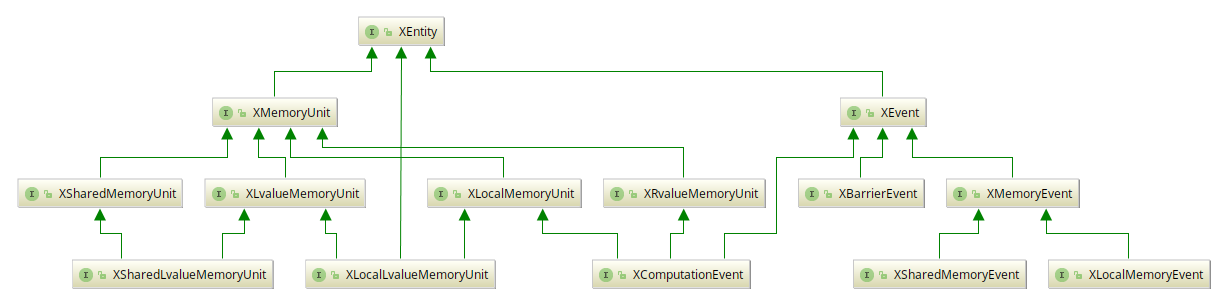
\includegraphics[width=\textwidth,height=\textheight,keepaspectratio]{img/my/class-diagrams/XEntity.png}
  \caption{TODO}
  \label{fig:class-diagrams:XEntity}
\end{figure}

\lstinputlisting{inc/XEventVisitor-cleaned.java}


%todo: some words on necessity of contexts and lack of them. How would we implement them

%todo: rename Interpreter -> Compiler.

%note https://en.wikipedia.org/wiki/Semantics_(computer_science)
%Operational semantics loosely corresponds to interpretation,

- hierarchy of Compilers (XCompiler is an stateful abstract machine)

- interface that it provides

- dependencies on other modules (memory-manager, etc.)


\subsection{Pre-compilation}
\label{ch:impl:y2x:precomp}

- collect goto labels (not done yet.)

- determine kind of variables (cannot be done during parsing? don't say this)


%todo: after all, list which modules (classes, managers) are being initialised during the pre-compilation. I'ts good to have the dependencies graph on moduls (operational semantics:) )

%\subsection{Compilation}
%\label{ch:impl:y2x:compil}

- more low-level code representation (or high-level assembly); abstract assembly language. refer to the %2_wmm.tex

- X-hierarchie


%\subsection{Post-compilation}
%\label{ch:impl:x2y:postcomp}

transformations

- After we acquired the event-based representation, we can perform some modifications/simplifications/optimisations on it (separately, allowing user to manage them)

- converting to SSA form (now: during the encoding. should be: during the post-compilation) (as one of necessary steps before encoding)

- setting up backward edges

- more?

- unrolling: why we cannot encode cyclic structures. reference to the paper (see arXiv version)
% If the analysing program contains a loop, then its control-flow graph represents the cyclic directed graph. Although, in order to be able to encode such a cyclic structure as a boolean formula, this graph needs to be

The original program encoded into the \texttt{XGraph} represents a \textit{flow graph}, a connected cyclic directed graph with single source node \texttt{(ENTRY)} (usually for convenience all leaves are connected to the sink node \texttt{(EXIT)}). The cycles are caused by low-level jump instructions, obtained from non-linear high-level control-flow statements (such as \texttt{while}, \texttt{do-while}, \texttt{for}, etc.). However, the cyclic flow graph cannot be encoded into SMT formula since ...
//TODO:REFERENCE.%TODO



\begin{figure}
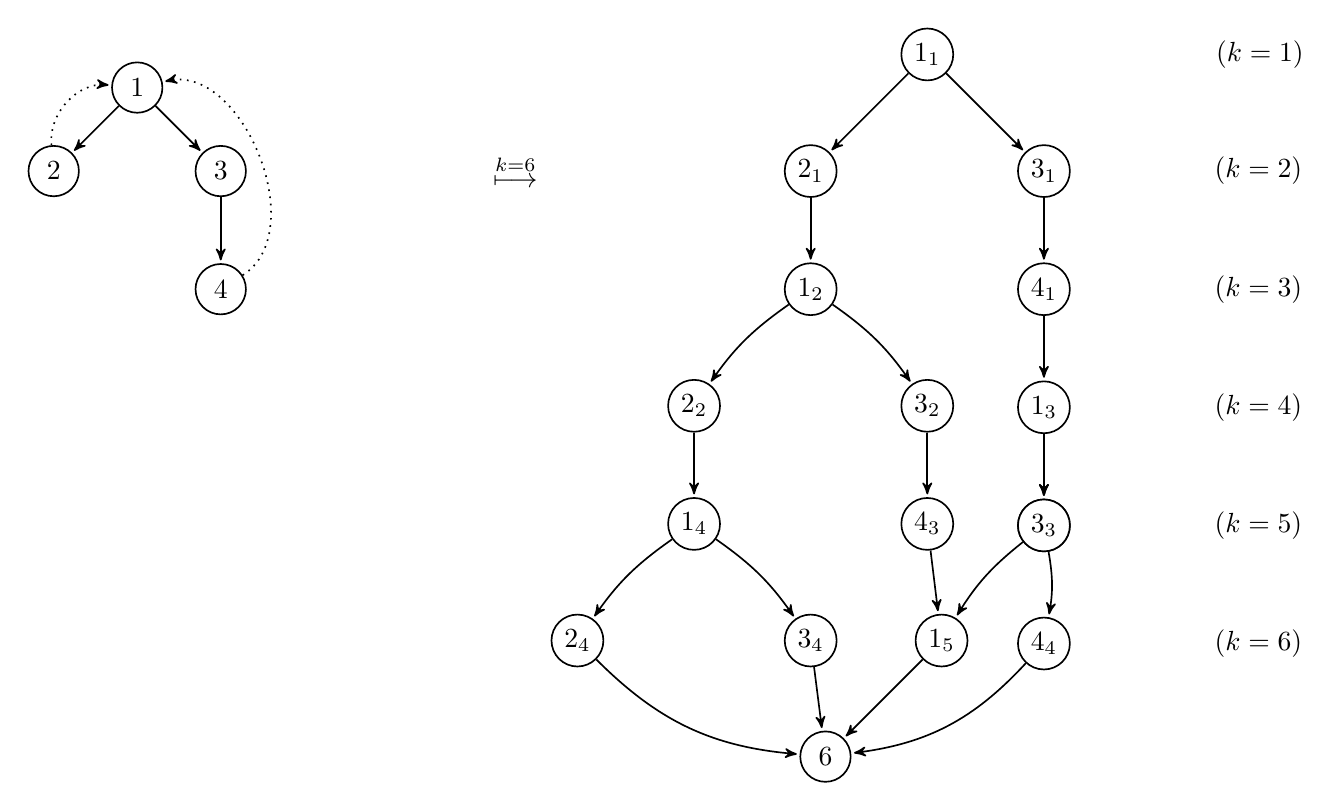
\begin{tikzpicture}[->,>=stealth',shorten >=1pt,auto,node distance=1.5cm,semithick]
\node[c] (1) [] {$1$};
\node[c] (2) [below left of=1] {$2$};
\node[c] (3) [below right of=1] {$3$};
\node[c] (4) [below of=3] {$4$};
\path[->]
(1) edge [] node {} (2)
(2) edge [bend left=50,dotted] node {} (1)
(1) edge [] node {} (3)
(3) edge [] node {} (4)
(4) edge [bend right=80,dotted] node {} (1)
;
\node[draw=none] (impl) [right=3cm of 3] {$\overset{k = 6}{\longmapsto}$};
;
\node[c] (21) [right=3cm of impl] {$2_1$};
\node[c] (11) [above right=1cm and 1cm of 21]{$1_1$};
\node[c] (31) [below right=1cm and 1cm of 11] {$3_1$};
\node[c] (41) [below of=31] {$4_1$};
\node[c] (12) [below of=21] {$1_2$};
\node[c] (22) [below left=1cm and 1cm of 12] {$2_2$};
\node[c] (32) [below right=1cm and 1cm of 12] {$3_2$};
\node[c] (13) [below of=41] {$1_3$};
\node[c] (14) [below of=22] {$1_4$};
\node[c] (43) [below of=32] {$4_3$};
\node[c] (23) [below of=13] {$2_3$};
\node[c] (33) [below of=13] {$3_3$};
\node[c] (24) [below left=1cm and 1cm of 14] {$2_4$};
\node[c] (34) [below right=1cm and 1cm of 14] {$3_4$};
\node[c] (15) [below right=1cm and -0.3cm of 43] {$1_5$};
\node[c] (44) [below of=33] {$4_4$};
\node[c] (6) [below left=1cm and 1cm of 15] {$6$};
\node[] (11k) [right=3.2cm of 11] {$(k = 1)$};
\node[] (31k) [right=1.7cm of 31] {$(k = 2)$};
\node[] (41k) [right=1.7cm of 41] {$(k = 3)$};
\node[] (13k) [right=1.7cm of 13] {$(k = 4)$};
\node[] (33k) [right=1.7cm of 33] {$(k = 5)$};
\node[] (44k) [right=1.7cm of 44] {$(k = 6)$};
\path[->]
(11) edge [] node {} (21)
(11) edge [] node {} (31)
(31) edge [] node {} (41)
(21) edge [] node {} (12)
(12) edge [bend right=10] node {} (22)
(12) edge [bend left=10] node {} (32)
(41) edge [] node {} (13)
(22) edge [] node {} (14)
(32) edge [] node {} (43)
(13) edge [] node {} (23)
(13) edge [] node {} (33)
(14) edge [bend right=10] node {} (24)
(14) edge [bend left=10] node {} (34)
(43) edge [] node {} (15)
(33) edge [bend right=10] node {} (15)
(33) edge [bend left=10] node {} (44)
(24) edge [bend right=20] node {} (6)
(34) edge [] node {} (6)
(15) edge [] node {} (6)
(44) edge [bend left=20] node {} (6)
;
\end{tikzpicture}
\label{fig:loop-unwind}
\caption{Example of the flow graph from Figure~\ref{fig:merged-loop.....}, unwinded up to the bound $k = 6$}
\end{figure}




%\section{XGraph to ZFormula (SMT) encoder}
%\label{ch:impl:comp:zformula}

- Then, this modified event-representation is being encoded to SMT formula and sent to the solver.



% say something about equals() and hashCode()



%TODO: \section{Optimisations}

\chapter{Evaluation}
\label{ch:eval}


\section{Comparison with \porthos[1]}
\label{ch:eval:show}

\subsection{Compilation and unrolling}
\label{ch:eval:show:compil}

%As an example of the compilation and unrolling processes, consider the simple
%As a simple example of the compilation process discussed in Section~\ref{ch:impl:proc:x-compiler}, 
Consider two equivalent functions in C (left) and the \porthos[1] input language (right) represented in Figure~\ref{ex:test-both-cf}. %(in the C language on the left-hand side, the \porthos[1] input language on the right-hand side).
%The functions are state-equivalent (represent the same state machine) and 
The functions does not compute any useful value, however they contain three nested \texttt{while}-loops and thus can serve as an illustration of the differences in the program compilation and unrolling between \porthos[1] and \porthos[2].
%contains several syntactic elements (such as prefix increment and loop-breaking statements), which are supported by \porthos[2] comparing to its predecessor.
%In the Figure, the control-flow subgraph \xgraph[CF] of the non-unrolled event-flow graph is presented on the right-hand side (

\begin{figure}[!h]
%\begin{minipage}{.53\textwidth}
\begin{subfigure}[b]{.53\textwidth}\centering
\begin{lstlisting}[language=Java,basicstyle=\ttfamily\small]

void t0(int &x) {
     int a = 1;
     int c = 1;
     while (a == 1) {
         int b = 1;
         while (b == 1) {
             while (c == 1) {
                 x = c;
             }
             x = b;
         }
     }
     x = a;
 }
 
 
\end{lstlisting}
\caption{An example in the C language}
\label{ex:both-cf:ptsC}
\end{subfigure}
%\begin{minipage}{.45\textwidth}
\begin{subfigure}[b]{.45\textwidth}\centering
\begin{lstlisting}[language=Java,basicstyle=\ttfamily\small]
{ x }
thread t0 {
     a <- 1;
     c <- 1;
     while (a == 1) {
         b <- 1;
         while (b == 1) {
             while (c == 1) {
                 x := c
             };
             x := b
         };
     };
     x := a
 }
\end{lstlisting}
\caption{An example in the \porthos[1] input language}
\label{ex:both-cf:pts1}
\end{subfigure}
\caption{Example: A demonstrative cyclic function}
\label{ex:test-both-cf}
\end{figure}

The functions are processed by \porthos[2] or modified version \porthos[1] that is able to print same \xgraph[CF] as the new tool (for that, the control-flow instructions \texttt{if-then-else}, \texttt{while} and \texttt{sequence} are expanded recursively and the head and the tails of each instruction are bind by the method processing its parent).
The graph generation is performed via the open-source library \texttt{Graphviz}~\cite{ellson2001graphviz}).
%Each event of the control-flow graph contains the unique number (generated by the \texttt{hashCode} method) in curly brackets below the value, which is necessary for correct displaying the graph.

The Figure~\ref{ex:test-both-pic} illustrates the data structure which the functions in Figure~\ref{ex:test-both-cf} are compiled to.
The left-hand side picture represents the non-unrolled \xgraph[CF] generated by \porthos[2], and the right-hand picture represents the AST generated by \porthos[1].

In both pictures, the writes are denoted with the left-directed arrow `\lstinline{<-}', and the functions \lstinline{load} and \lstinline{store} denote the type of the shared memory event.
The primary transitions that denote unconditional jumps or if-true-transitions are pictured with solid lines, and the alternative transitions that denote if-false-transitions are pictured with dotted lines.
The graphs contains a single source event and a single sink event represented by the grey triangles (actually, the graph produced by \porthos[1] does not have sink and source nodes, but they were added to the picture for demonstrative purposes).
For clarity, all branching events, that in current example serve as the conditional events of loops, are highlighed with light-grey colour.

\begin{figure}[!h]
%
\begin{subfigure}[t]{.49\textwidth}\centering
  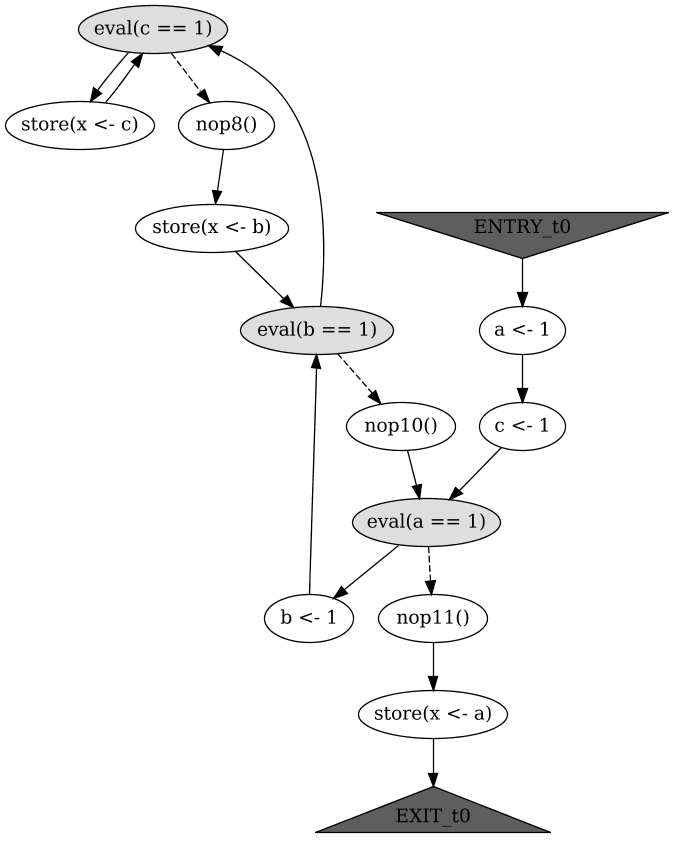
\includegraphics[width=\textwidth,keepaspectratio]{img/my/graphs/unrolling-comparison/PorthosC/t0.png}
  \hfill
  \caption{The compiled \xgraph{} of the function in Figure~\ref{ex:both-cf:ptsC}}
  \label{ex:both-cf:graph:ptsC}
\end{subfigure}
%
\begin{subfigure}[t]{.49\textwidth}\centering
  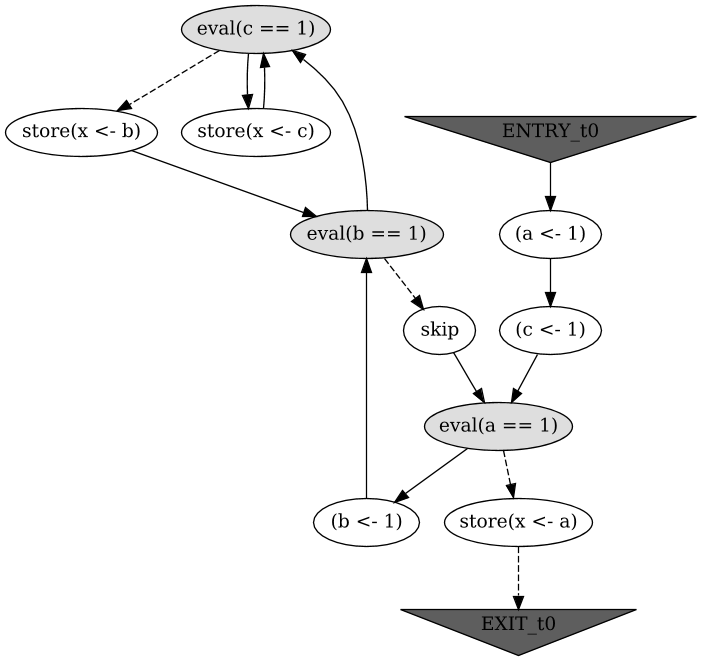
\includegraphics[width=\textwidth,keepaspectratio]{img/my/graphs/unrolling-comparison/Porthos/t0.png}
  \hfill
  \caption{The compiled AST of the function in Figure~\ref{ex:both-cf:pts1}}
  \label{ex:both-cf:graph:pts1}
\end{subfigure}
%
\caption{The control-flow graphs of the functions represented in Figure~\ref{ex:test-both-cf}}
\label{ex:test-both-pic}
\end{figure}

Two compiled the graphs are equivalent up to the extra \texttt{nop}-events in the \porthos[2] graph, that are necessary for correct encoding as it was discussed in Section~\ref{ch:enc:bmc:cf}, and \texttt{skip}-events in \porthos[1] graph.
However, the unrolled graphs presented in Figure~\ref{ex:test-both-pic-unroll} are different as \porthos[2] uses different unrolling algorithm.
The labels of events in the left-hand side picture (produced by \porthos[2]) are augmented by the unrolling depth number, which is separated from the event label by comma.

The unrolling algorithm used by \porthos[1] (right-hand side picture) unrolls \textit{all} loops $k$ times (where $k$ is the unrolling bound), and the unrolling algorithm of \porthos[2] unrolls loops so that not more than $k$ events are executed.
As it is illustrated by the picture, the new algorithm produces a better set of program executions (for example, the unrolled graph of \porthos[1] does not contain executions of the inner loops more than $k=2$ times, which makes the old unrolling algorithm not complete).
As the new unrolling algorithm uses the Deep-First Search, it discovers \textit{all} possible paths, therefore the result graph contains \textit{all} possible executions and thus is complete.

Note that the unrolled graph produced by \porthos[2] does not necessarily become a tree after removing the sink node.
Some branches of the graph are merged when the executions have the same event with the same unrolling depth number.
For example, primary transitions of both events `\lstinline{[b <- 1, 8]}' and `\lstinline{[store(x <- b), 8]}' (produced by executions of the first iteration of the \texttt{while} loop) lead to the same event `\lstinline{[eval(b == 1), 9]}' (the first event of the second iteration of the second loop).

\begin{figure}[!h]
%
\begin{subfigure}[b]{.6\textwidth}\centering
  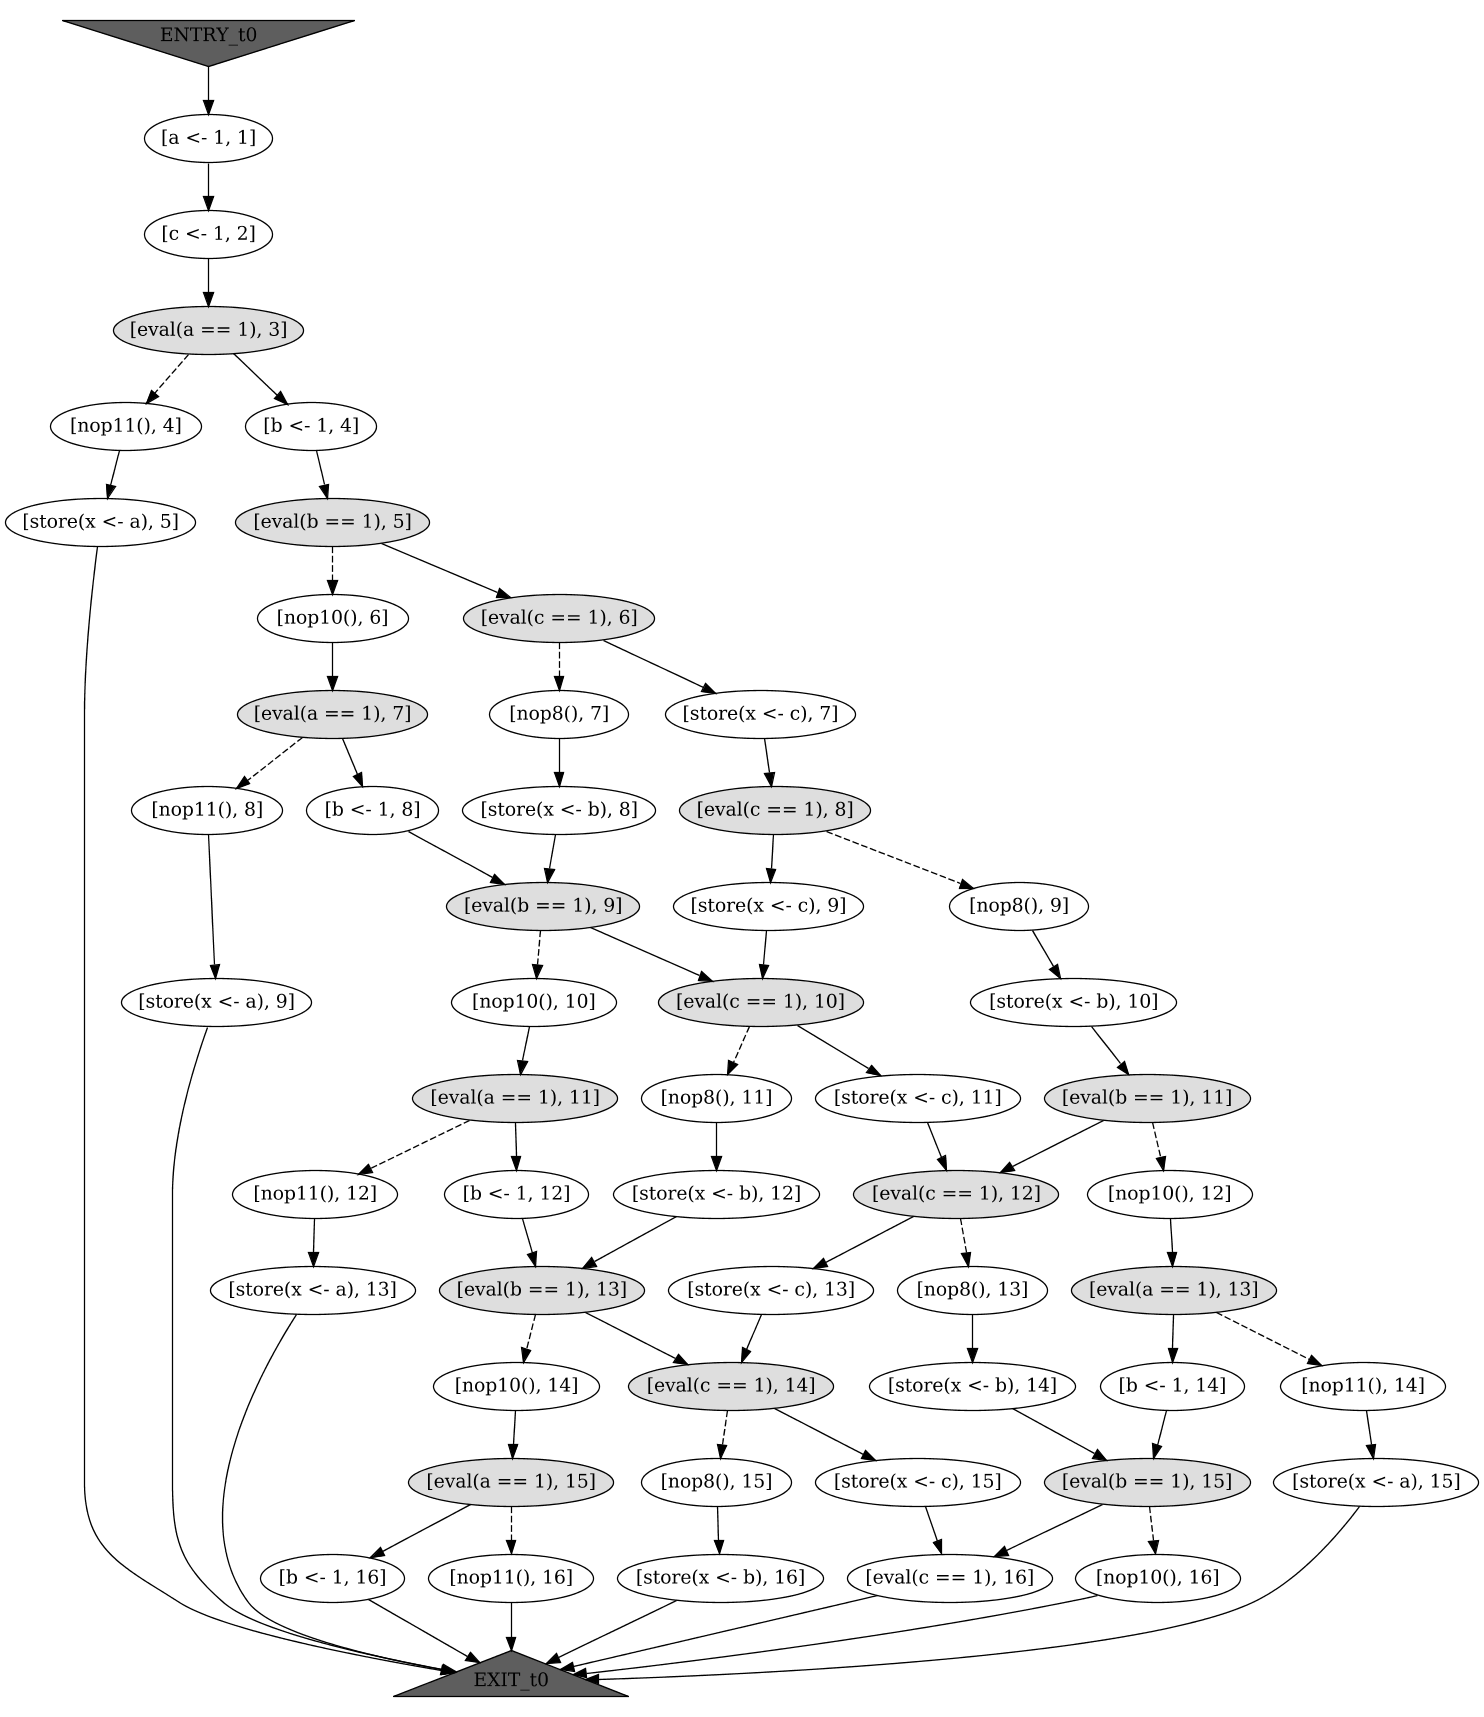
\includegraphics[height=.6\textheight,width=\textwidth]{img/my/graphs/unrolling-comparison/PorthosC/t0_unrolled.png}
  \hfill
  \caption{The unrolled \xgraph{} of the function in Figure~\ref{ex:both-cf:ptsC}}
  \label{ex:both-cf:graphU:ptsC}
\end{subfigure}
\hfill
%
\begin{subfigure}[b]{.3\textwidth}\centering
  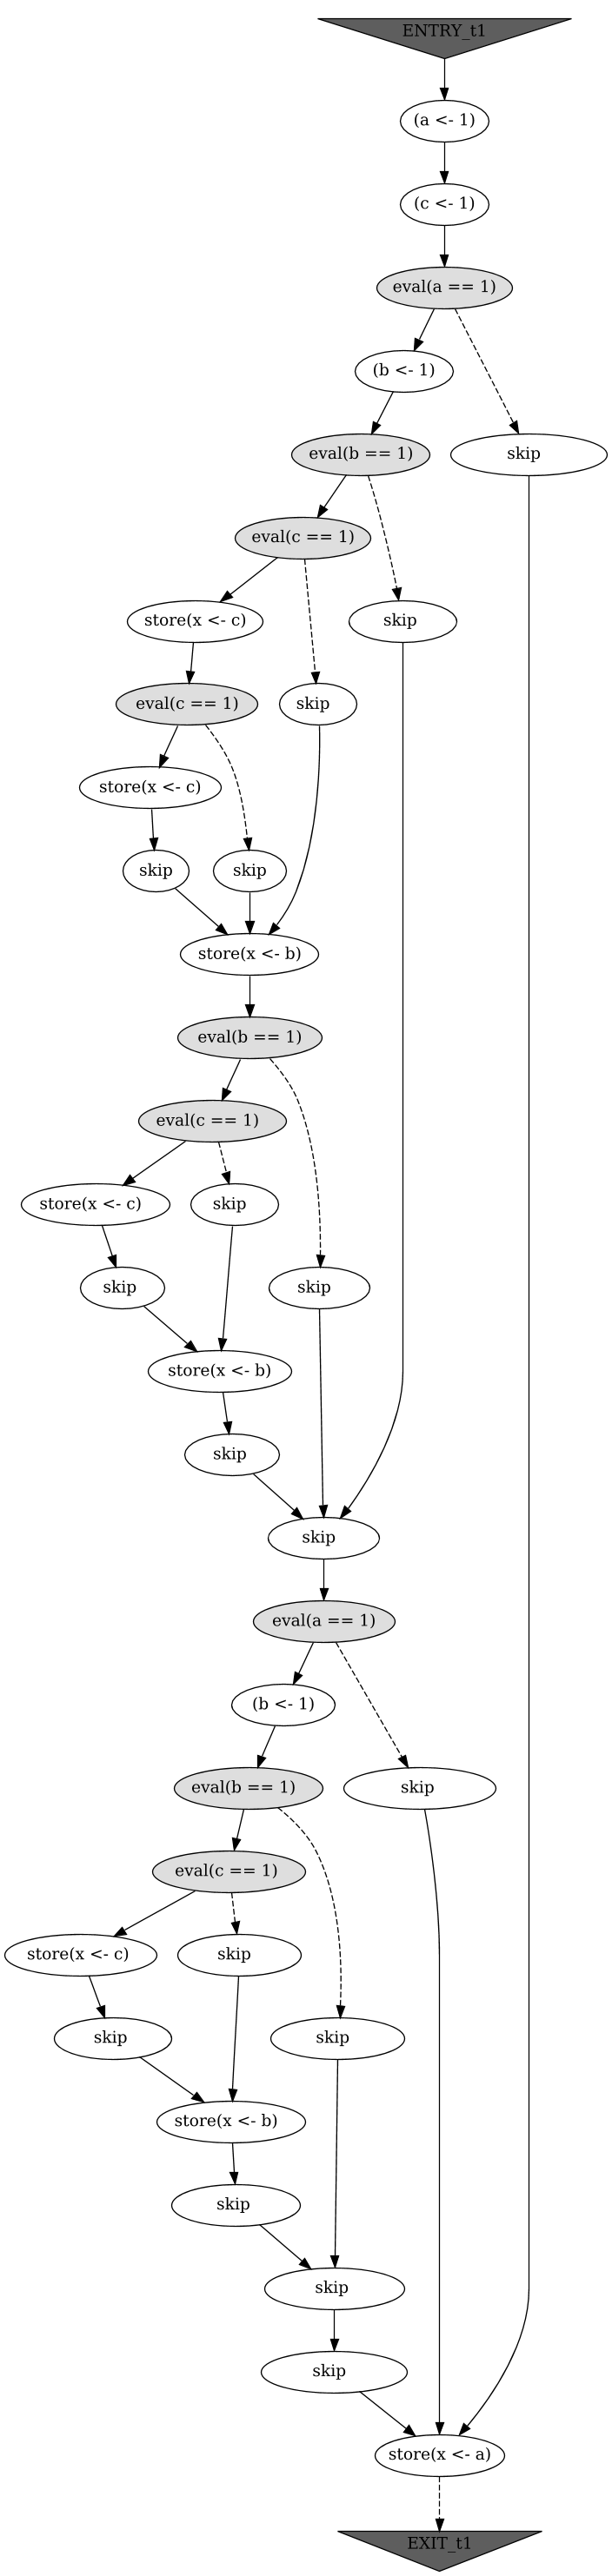
\includegraphics[height=.9\textheight,width=\textwidth]{img/my/graphs/unrolling-comparison/Porthos/t0_unrolled.png}
    \caption{The unrolled AST of the function in Figure~\ref{ex:both-cf:pts1}}
    \hfill
  \label{ex:both-cf:graphU:pts1}
\end{subfigure}
\hfill
%
\caption{The unrolled control-flow graphs of the functions represented in Figure~\ref{ex:test-both-cf}}
\label{ex:test-both-pic-unroll}
\end{figure}

%The arguments \lstinline{x} and \lstinline{y} of the function are passed by reference, therefore they are treated as global variables.
%The local variable declaration `\lstinline{int r;}' produces no events (it is processed by the X-graph pre-compiler that invokes the memory manager to create the new local variable \lstinline{r}).
%The first event `\lstinline{load(reg_tmp0 <- x}' loads the value of the global variable \lstinline{x} into the temp register \lstinline{reg_tmp0} in order to satisfy the requirement that all computation must be performed over local variables;
%note that each element of the computational tree `\lstinline{eval(eval(eval(5 + eval(eval(4 / 2) * reg_tmp0)) % 3) == 1)}' is represented by a local memory unit (either \texttt{XComputationEvent} or \texttt{XConstant} or \texttt{XRegister}).
%The node of this computational event in the control-flow graph has two outgoing edges, the primary edge to the `\lstinline{load(reg_tmp1 <- y}', the first event of the then-branch of the while-loop, and the alternative edge to the \lstinline{nop}-event representing the only event of the else-branch.

%As is was discussed in Section~\ref{ch:impl:model:xgraph}, all computation events have no impact to the global state of the concurrent system.
%Therefore, the interpreter does not \textit{emit} computational events, but it \textit{creates} them.
%This means, when the \texttt{Y2XConverterVisitor} processes the expression tree `\lstinline{(5 + 4/2 * x) 3 == 1}', it calls the method \texttt{createComputationEvent} of the interpreter that only creates the computation event and does not change its state.
%However, once the converter meets the global variable \lstinline{x}, it calls the interpreter method \texttt{emitMemoryEvent} to copy its value to a temp register; since it meets the global variables involved to the computation before it ends to process the whole computation expression, the values of all these global variables will be copied to temp registers \textit{before} the computation expression is used by any other event.
%Note that if the computation expression has not been used by any other event (for example, as the constant \lstinline{1} in the following C code: `\lstinline{foo(); 1; bar();}'), it is lost from the model (by the term \textit{use} here we mean that the computation event is evaluated as a guard or assigned to another memory unit).


%\subsection{The X-graph unrolling}
%\label{ch:eval:show:unrol}

%Once the \xgraph[CF] is constructed, it should be unrolled to an acyclic flow-graph (as it was discussed in Section~\ref{ch:impl:proc:x-unroll}).
%The Figure~\ref{ex:unrolling} shows the control-flow subgraph \xgraphU[CF] of the event-flow graph from the previous example (see Figure~\ref{ex:compilation}) unrolled up to bound $k=16$.
%


%TODO: here (or better in Chap 5 ) say about 'we tried different encoding schemes !!!!!!!!!!!!!!!!!!!!!!!!!!!!!!!!!!!!!!!!!!!!!!!!!!!!!!!!!!!!!!!!!!!!!!!!!!!
 
%Also note that comparing to the unrolling bound description given in Section~\ref{ch:impl:proc:x-unroll}, 
%As the distinction between complete and incomplete sink nodes is not implemented yet, 

%\begin{figure}[!h]
%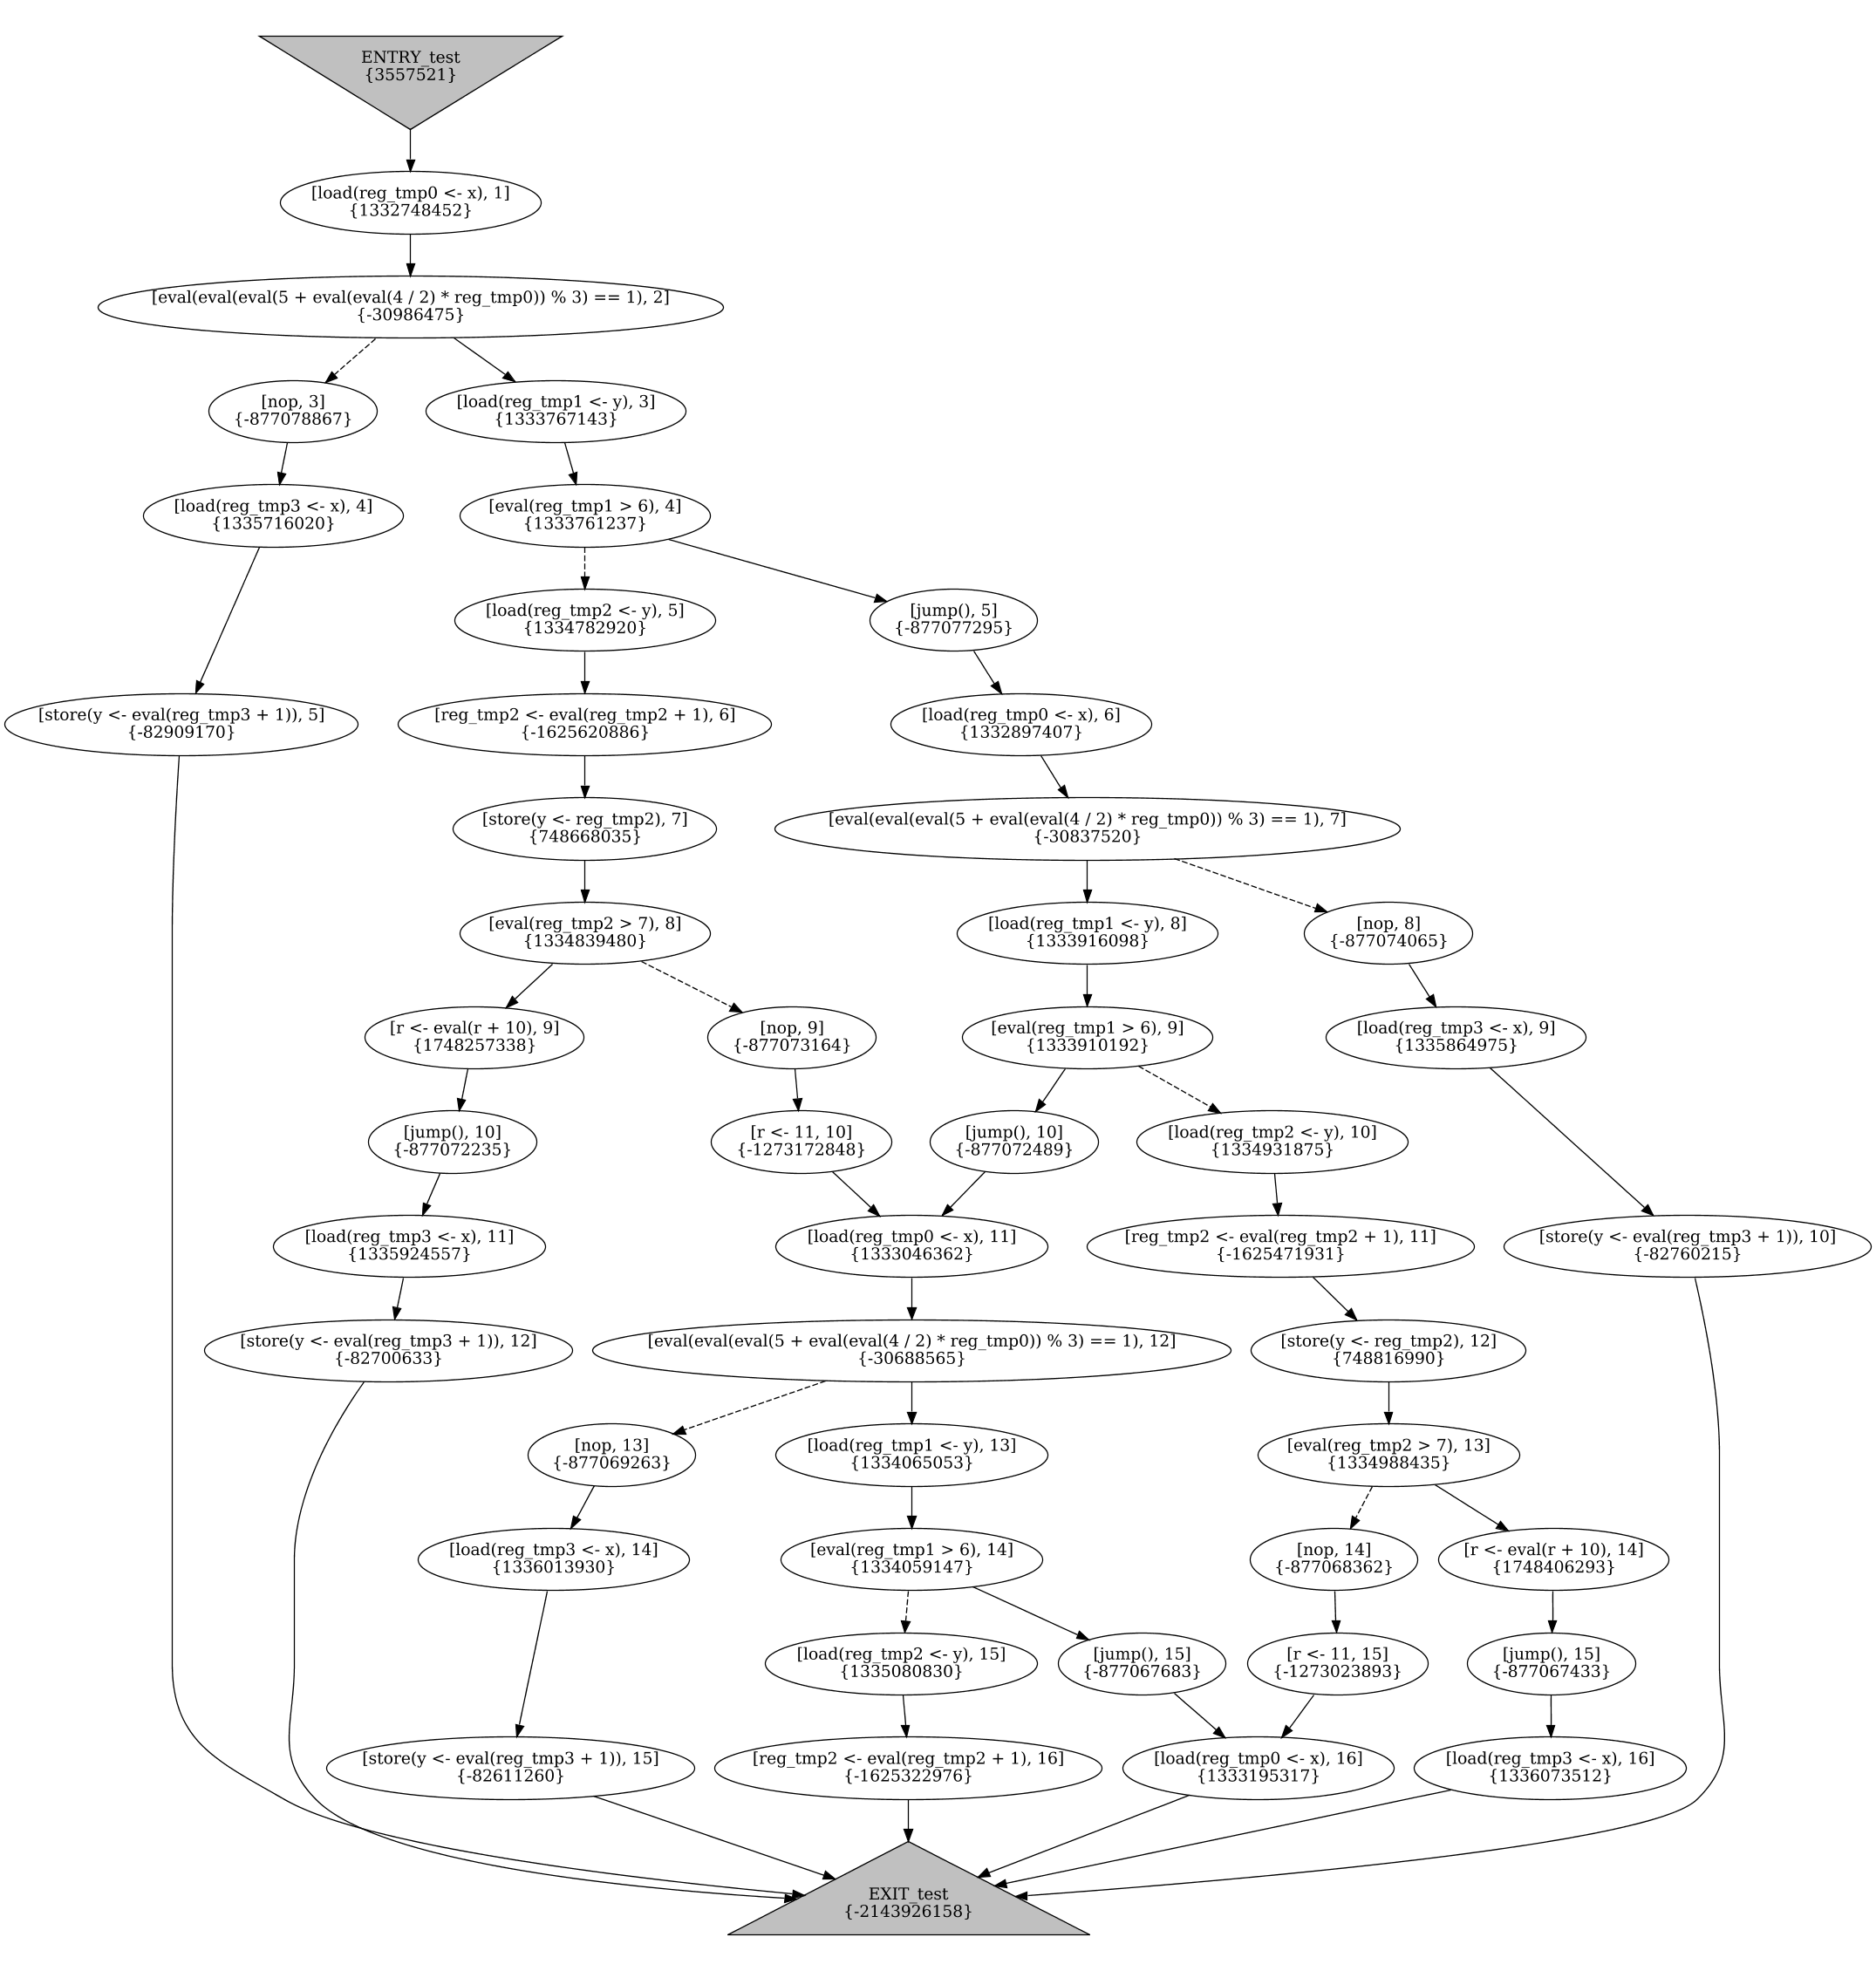
\includegraphics[width=\textwidth,height=\textheight]{img/my/graphs/test_unrolled.png}
%\caption{Unrolling of the event-flow graph presented in Figure~\ref{ex:compilation}}
%\label{ex:unrolling}
%\end{figure}


\section{Performance evaluation}
\label{ch:eval:perf}

As an example of the C program liable for the reachability and portability analysis, consider the Dekker's algorithm for mutual exclusion of two processes, originally described by Dijkstra~\cite{dijkstra1962over}; the program is presented in Appendix~\ref{apx:dekker}.
For testing \porthos[1], we used the same file in old \porthos{} input language (\texttt{dekker.pts}), which was used in evaluation tests in the original paper~\cite{Porthos17a}.

\subsection{State reachability analysis}
\label{ch:eval:perf:reach}

%For checking reachability of the final states of the unrolled graphs compiled for a certain hardware architecture, the tool encodes both program and hardware memory model constraints as it was discussed in Section~\ref{ch:enc:bmc}.
%The result formula is then solved by the Z3 

%TO-DO: fix interface
%To run \porthos[2] in reachability analysis mode, we use the command `\lstinline{mousq

%\textbf{TODOOOOOOOOOOOOOOOOOOOOO!!!! Re-compute tests with new counting of encoding}
When running in the state reachability analysis mode, \porthos[2] produces the following output:

\begin{lstlisting}
$ java PorthosC --reachability --input benchmarks/C11/Dekker.c \
      --bound 27 --target TSO
0.288: Interpretation...
0.426: Unrolling...
0.533: Program encoding...
0.701: Program domain encoding...
#=193 (107)
34.187: Memory model encoding...
36.818: Solving...
{
  "result": "NonReachable",
  "mainTimer": {
    "elapsedTimeSec": 36.163
  },
  "timers": {
    "Interpretation": {
      "elapsedTimeSec": 0.132
    },
    "ProgramDomainEncoding": {
      "elapsedTimeSec": 32.486
    },
    "Solving": {
      "elapsedTimeSec": 0.345
    },
    "Unrolling": {
      "elapsedTimeSec": 0.061
    },
    "MemoryModelEncoding": {
      "elapsedTimeSec": 2.631
    },
    "ProgramEncoding": {
      "elapsedTimeSec": 0.168
    }
  },
  "errors": []
}
\end{lstlisting}

For time benchmarking we ran the tool $5$ times and computed the median of the encoding time.
Benchmarking was performed on the Linux machine 8-core Intel(R) Core(TM) i7-3632QM CPU @ 2.20GHz, Java(TM) SE Runtime Environment (build 1.8.0\_161-b12) (Java virtual machine was configured by default parameters).
The time was measured by the tool itself via the native Java method \texttt{System.currentTimeMillis}.

%For \porthos[1] we specify the unrolling bound $k_1 = 2$, and for \porthos[2] the bound is $k_2 = 21$ ().
As the unrolling algorithm has been changed, the number of events after unrolling differs considerably.
Therefore, the correct performance comparison with \porthos[1] is not manageable as the performance of the tools depends directly on number of events.
For example, with the bound $k_1=2$ \porthos[1] produces $59$ events (among them, $51$ shared-memory events) with the program domain encoding time 4.608 sec,
and with the bound $k_1=3$ \porthos[1] produces $95$ events (among them, $107$ shared-memory events) with the program domain encoding time 21.475 sec;
whereas \porthos[2] with the bound $k_2=17$ produces $57$ ($31$) events with the program domain encoding time 1.734, and with the bound $k_2=27$ it produces $193$ events (among them, $107$ shared-memory events, which equal to the number of shared-memory events produced by \porthos[1] with the bound $k_1=3$) with the time 32.673 sec.
Therefore, the new unrolling scheme has made the analysis complete but at the same time it reduced the performance considerably.
%The last result shows that with the bounds $k_1=3$ and $k_2=27$ both tools have executed same number of loops  almost equivalent as they
%However, the program domain encoding and memory model encoding schemes have not been changed considerably comparing to \porthos[1], therefore the execution time 
%Although, the performance depends directly on number of events, 

%\porthos[2] shows the full encoding time for the Dekker's algorithm 2.699 sec (from which 0.152 sec spent for the program encoding, and other part spent for the memory model encoding).
%In contrast, \porthos[1] shows the encoding time 6.152 sec (from which 0.223 sec spent for the program encoding). %, which is considerably better result.
%Thus, the performance of the encoding stage has been\textbf{ improved in 2.7 times}.

Note that the time spent by \porthos[2] for the interpretation and unrolling stages remains to be negligible comparing to the full encoding time.
Therefore, we conclude that the new architecture implies no performance overhead comparing to the previous version of the tool.
The time spent by the SMT-solver while considering the SMT-formula encoded by \porthos[2] was 0.039 sec, and in case of \porthos[1] the time was 1.291 sec.
The number of events in the event-flow graph of \porthos[2] is 82 events (among them 59 memory events), and the number of events encoded by \porthos[1] is 95 (among them 51 memory events).
Even though the number of memory events processed by \porthos[1] was less, the time of solving the result SMT-formula was significantly more.

<TODO: above as table>

%We consider this improvement to be the result of some technical optimisations applied to the encoding stage of \porthos[2].
%The major optimisation is the \textit{memoisation} of frequently requested calls.
%For example, the code of \porthos[1] contains 39 calls that take the subset of a set of events, 10 of them are performed in a loop over all events (in \texttt{Domain.encode} method of \porthos[2]).
%The pattern is the following: `\lstinline{program.getEvents().stream().filter(e -> e instanceof MemEvent || e instanceof Local).collect(Collectors.toSet())}'.
%%TODO: refactor X-program inheritance
%In \porthos[2], these calls were replaced by the lazily initialisable memoisation methods (see \texttt{XProgram}): \\
%
%\vspace{-1em}
%\begin{lstlisting}[language=Java]
%public ImmutableSet<XMemoryEvent> getMemoryEvents() {
%    return memoryEvents != null
%        ? memoryEvents
%        : (memoryEvents = getAllNodesExceptSource(XMemoryEvent.class));
%}
%\end{lstlisting}

%TODO: say how much the \textit{immutable data structures} helped (as it was discussed in Chapter~\ref{ch:impl}).

%<TODO: compare numbers of clauses of SMT-formulas>

<TODO: profile both programs, say sth about memory usage!> 


\subsection{Portability analysis}
\label{ch:eval:perf:port}

For evaluating the tool working in the portability analysis mode, we used the same file \texttt{Dekker.c} tested for the state-portability from TSO to SC: %TODO: Say sth about state-portability

%!!! \textit{\textbf{TODO: change the main class name to PorthosC }} !!!

\begin{lstlisting}
$ java PorthosC --portability --input benchmarks/C11/Dekker.c \
      --bound 27 --source TSO --target SC --state
0.359: Interpretation...
0.364: Unrolling...
0.590: Unrolling...
0.623: Program encoding...
0.847: Program domain encoding...
#=193 (107)
#=193 (107)
66.541: Memory model encoding...
72.321: Solving...
{
  "result": "StatePortable",
  "iterations": 0,
  "mainTimer": {
    "elapsedTimeSec": 73.02
  },
  "timers": {
    "ProgramEncoding": {
      "elapsedTimeSec": 0.223
    },
    "MemoryModelEncoding": {
      "elapsedTimeSec": 5.779
    },
    "Interpretation": {
      "elapsedTimeSec": 0.248
    },
    "Solving": {
      "elapsedTimeSec": 0.699
    },
    "ProgramDomainEncoding": {
      "elapsedTimeSec": 65.693
    },
    "Unrolling": {
      "elapsedTimeSec": 0.022
    }
  },
  "errors": []
}
\end{lstlisting}

As the portability analysis requires compiling the program under two memory models, the overall program domain encoding time 65.693 sec is almost double as the same time in reachability analysis mode (\porthos[1] shows program domain encoding time 41.027 sec with the bound $k_1=3$).


\subsection{New features}
\label{ch:eval:perf:feat}

%The revised design of \porthos{} tool includes the following new features:
Apart from redesigning the tool architecture and extending the input language, we added support for basic constructions used in \textit{Kernel litmus tests}~\cite{alglave2018frightening}.
Although, current version of \porthos[2] only supports some basic macros of the Linux kernel (such as \texttt{READ\_ONCE} and \texttt{WRITE\_ONCE} for atomic load and store with relaxed memory ordering) as the support for kernel-specific memory barriers goes out of the scope of current thesis.
Note that, comparing to the \porthos[1], adding support for new functions in \porthos[2] does not require changing the input language grammar, this is carried by invocation hooking mechanism described in Section~\ref{ch:impl:proc:x-compiler}.

As an example, consider the SB litmus test for the Linux kernel (which is similar to the one presented in Figure~\ref{simple_wmm_x86}):
\begin{lstlisting}
{ int x = 0; int y = 0;}

P0(volatile int* y, volatile int* x) {
  int r0;
  WRITE_ONCE(*x,1);
  r0 = READ_ONCE(*y);
}

P1(volatile int* y, volatile int* x) {
  int r0;
  WRITE_ONCE(*y,1);
  r0 = READ_ONCE(*x);
}

exists(x == 0 && y == 0)
\end{lstlisting}

If verifying this litmus test by \porthos[2] in the state reachability mode, the test passes for TSO memory model and fails for SC model.


\chapter{Conclusion}
\label{ch:summary}

%instead of extending the \textit{grammar} of input language, we extended the \textit{architecture} of the tool so that the full C language can be supported

\section{Solved tasks and contributions}

During the work on this thesis, we solved the following engineering and scientific tasks:

%TODO: written a generic hardware-agnostic extensible non-optimising compiler

\begin{enumerate}[label=\arabic*.] %[label=\Roman*.]
\item
We have studied existing weak memory model-aware analysis approaches, tools and frameworks to gather deep understanding of the problem (Sections~\ref{ch:intro:related} and~\ref{ch:enc:mc} and Chapter~\ref{ch:wmm}).

\item
Then, we explored existing implementation of the portability analysis tool \textit{\porthos{}} and designed the new tool \textit{\porthos[2]} that accepts as input the larger subset of the C language and supports its fundamental concepts by design, has modular architecture and disposes the extensible knowledge base of the domain-specific functions.
The key aspects of the architectural design and implementations are the following:

  \begin{enumerate}[leftmargin=\parindent,label=\alph*.]
  \item The first stumbling block in extension of the input language was the \porthos[1] program input parser, which performs the full semantic analysis of the program.
  Although it works for a small subset of the C language, the rich and expressive language such as C requires several stages of analysis before the compilation stage.
  To handle this, we implemented the processing units that analyse the AST of the program on the \textit{pre-compilation} stage (see Section~\ref{ch:impl:proc:x-pre-compiler}).

  As an example, the \textit{variable kind analysis} (shared or local) is performed by \porthos[1] syntactically, depending on the operator or the function that uses the variable.
  In contrast, \porthos[2] traverses the program AST and collects information of all variables accessed in the program during the pre-compilation stage (see Section~\ref{ch:impl:proc:x-pre-compiler}).
  Currently, \porthos[2] considers a variable to be shared if it was declared as a pointer, or its address is accessed at least once by the code of any process, or it was declared as a parameter of the function that defines a process, or it was exported by \texttt{extern} keyword or an exporting function.

  \item In addition, \porthos[2] supports \textit{new syntactic constructions} of the C language: \texttt{break} and \texttt{continue} jumps, function invocations, multiple-variable declarations (as `\lstinline{int a, b=2, z;}'), arbitrary expressions allowed by the C11 standard~\cite{c11}, and some others (see Section~\ref{ch:impl:input}).

  \item As the C language supports unconditional \texttt{goto}-jumps, the control-flow graph can have an arbitrary structure, which can not be modelled solely by the program AST, therefore \porthos[2] compiles the AST to the low-level hardware-agnostic program representation \xgraph{}.
  For that, we implemented the \textit{full C interpreter} discussed in Section~\ref{ch:impl:proc:x-compiler}.
  
  \item Originally, the control-flow instructions were encoded directly into the SMT-formula~\cite{Porthos17a}.
  In contrast, \porthos[2] encodes the low-level \xgraph{} representation in accordance with the \textit{new control-flow encoding scheme} that in general follows the one proposed in~\cite[Chapter 5.1.2]{heljanko2008unfoldings} (see Section~\ref{ch:enc:bmc:cf}).
  As the new encoding scheme does not add new variables to every control-flow instruction, the number of variables in the result SMT-formula is expected to be smaller.
  
  \item Since \porthos[2] compiles the program AST to the \xgraph{} before encoding it into the SMT-formula, we decided to change the \textit{unrolling algorithm} from unwinding all loops $k$ times (where $k$ is the user-specified unrolling bound) to the DFS-based algorithm that explores \textit{all possible executions} that the program can produce within $k$ steps (see discussion on the unrolling in Sections~\ref{ch:impl:proc:x-unroll} and~\ref{ch:eval:show:compil}).
  On the other hand, it is shown in Section~\ref{ch:eval:show:unrol} that the implementation of the new unrolling algorithm does not produce exponentially many dummy \texttt{nop}-events as the implementation of the old unrolling algorithm does.
  Another benefit of the new unrolling scheme is that it is much more configurable (i.e., the number of events grows gradually as the unrolling bound is being increased, see Figure~\ref{dep:events}). \\
  Although the new unrolling algorithm produces considerably more executions than the old one and thus requires more time for analysis, \porthos[2] uses the new unrolling algorithm by default as it is complete (finds all possible executions).

  \item For ease of adding support for new domain-specific functions (for example, the Kernel-specific atomic write function \texttt{atomic\_store}), we implemented the \textit{invocation hooking}, a flexible mechanism for intercepting the compilation process without changing the interpreter.
  The invocation hooking mechanism serves as a knowledge base for the program domain, that is to be filled and extended in future.
  Invocation hooks are defined in Java and thus are flexible, though their extension and modification requires some knowledge of the internals of the tool.
  We illustrate this mechanism with the basic support for Linux kernel litmus tests (see Sections~\ref{ch:impl:proc:x-compiler} and~\ref{ch:eval:perf:feat}).

  \end{enumerate}
  
\item 
As the tests show, the \textit{performance overhead} of the new architecture is negligible (see Section~\ref{ch:eval:perf}), therefore we consider the applied architectural changes as acceptable.

\end{enumerate}


\section{Limitations and directions for future work}

Current implementation of \porthos[2] has the following limitations, that might possibly define the direction of the future work.

\begin{itemize}[leftmargin=\parindent]
\item One of the major limitation of \porthos[2] as a software verification tool is its sensitivity to the \textit{combinatorial explosion} of the state space.
%that performs complete analysis
As it was shown in Section~\ref{ch:eval:perf}, the number of events of the unrolled program grow rapidly as the user increases the unrolling bound.
One possible way to reduce the number of the program states might be applying some traditional techniques that target the state explosion problem (such as concrete execution as a part of \textit{concolic execution}~\cite{majumdar2007hybrid} before the unrolling stage).
However, this must be done carefully and with taking into account the analysing weak memory model, because otherwise it can lead to the loss of states and thus to incorrect analysis results.
Nonetheless, the small-size litmus test-like programs (containing hundreds of events after the unrolling) remain to be handleable by \porthos[2] within reasonable time.
% cannot be applied to our problem \textit{before} the weak memory model is considered, 
%One possible enhancement, that could treat but not cure this flaw, could be an extra analysis stage carried before the unrolling, that analyses 

%\item As its predecessor, \porthos[2] does not propose any heuristic for finding the optimal unrolling bound.

\item For justifying the correctness of the verification that bases on the result of the input program unrolling (via the new unrolling scheme discussed in Section~\ref{ch:impl:proc:x-unroll}), one might want to be aware whether the execution in the unrolled event-flow graph has run the loop a whole number or it was interrupted on non-last event of the loop.
This can be modelled with two kinds of sink events (completed and uncompleted) of the event-flow graph as it was discussed in Sections~\ref{ch:enc:bmc:cf} and~\ref{ch:impl:proc:x-unroll}.

\item \textit{Extending the knowledge base} of domain-specific functions to model synchronisation primitives (the compiler mapping) can be considered as the main future research direction.
Thus, to be able to process most Linux kernel litmus tests, \porthos[2] needs to know the semantics of the barrier and memory operation functions that are specific for the Linux kernel in order to be able to compile them into the \xgraph{} and later encode them into the SMT-formula.
Due to modular architecture of \porthos[2], the extension of the knowledge base can be done by modifying solely the invocation hooking mechanism.
Note that the flip side of the flexibility of invocation hooks is their complexity: being written in Java, in addition they require from the user some knowledge of general architecture of the tool, the interface methods provided by the interpreter, the class hierarchy of the \xgraph{} elements, etc.

\item The wide range of existing litmus tests may require \porthos[2] to \textit{support new input languages}.
The first candidates for being supported are the LISA language (Litmus Instruction Set Architecture)~\cite{alglave2016syntax} and assembly languages of most common architectures (x86, POWER, Alpha, etc.).
Note that the programs in low-level languages can be easily compiled to the \xgraph{} representation by existing compiler architecture since low-level assembly-like languages can be considered as the subset of the C language, that restricts the set of non-linear control-flow instructions to the conditional and unconditional jumps (which are supported by the current \xgraph{} compiler of \porthos[2]).
%Note that adding support for low-level languages requires adding the new \xgraph{} compiler that will compile the low-level syntax tree (with non-conditional jumps as the only )

\item Although \porthos[2] has an extended support for primitive data types (integers, reals, booleans), it still is not able to handle the \textit{complex data types}.
However, as the \tool{Z3} solver supports the theory of constant-size arrays, it might be relatively easy to extend the support for constant-size arrays (declared as `\lstinline{int arr[10];}'), enumerations and structures.
Nevertheless, pointers and variable-size arrays (allocated in the heap by functions \lstinline{malloc}, \lstinline{calloc}, etc.) require a stronger pre-processing analysis before being encoded into an SMT-formula.

\item Currently, \porthos[2] can operate only in the intra-procedural analysis mode by assuming that each function provided by the user represents a separate thread (so-called litmus test-mode).
One future direction of the work could be adding the \textit{inter-procedural analysis mode} for scanning a code project instead of a separate file (see the discussion in Section~\ref{ch:impl:principles}).
Although, processing large programs may require serious memory optimisations (for instance, in storing the full unrolled graph data structure), which can possibly lead to worsening the overall performance.
In addition, when processing large code projects, \porthos[2] might need the memory-guarding module that tracks the memory consumption of the tool and aborts its work if necessary.

\item As it was mentioned in Section~\ref{ch:enc:bmc:cf} devoted to the encoding for the control-flow of the program, the new encoding scheme used by \porthos[2] allows to analyse \textit{partial functions}.
Although the current \porthos[2] interpreter infrastructure is not configured to perform a partial analysis, it can be easily supported.

\item During the implementation of \porthos[2], we have only done limited \textit{testing of the tool}.
Thus, in order to increase the stability of \porthos[2], we need to cover its code by unit- and functional tests.

\item One might want to compare the performance of \porthos[2] in cases of usage the different SMT-solvers.
For that, the \zformula{} abstraction layer will be useful as new SMT-solvers can be easily added (the general way to support multiple SMT-solvers is to convert the \zformula{} to an SMT-LIB formula~\cite{smt-lib}, that can be passed as input to the SMT-solver run as an external process).

%\item <parallelised>

%\item <C processor directives + typedef > 
%<TODO: a short summary here>

%\item <contexts for local mem units in mem manager>

%\item <as an optimisation, maybe use more comprehensive unrolling algo as in Aho>

%\item In order to be able to assess the A user might want to know

%\item optionally: urnolling algo; 

\end{itemize}


The new tool \porthos[2] with the extensible program domain knowledge base can be considered as a generalised framework for SMT-based memory model-aware analysis, which can not only perform the reachability and portability analysis, but also serve as a basis for other kinds of static analysis of concurrent programs.



\ifdefined\IsAalto
\else
  \cleardoublepage
  \phantomsection
  %
  \addcontentsline{toc}{chapter}{Abbreviations}
  \chapter*{Abbreviations}
% The longtable environment should break the table properly to multiple pages, if needed
\noindent
\begin{longtable}{@{}p{0.25\textwidth}p{0.7\textwidth}@{}}
API & Application Programming Interface \\
AST & Abstract Syntax Tree \\
BDD & Binary Decision Diagrams \\
BNF & Backus-Naur form \\
BMC & Bounded Model Checking \\
CF  & Control-Flow \\
CPU & Central Processor Unit \\
CTL & Computational Tree Logic \\
DF  & Data-Flow \\
DFS & Deep-First Search \\
DSA & Dynamic Single-Assignment form \\
DTO & Data-Transfer Object \\
LTL & Linear Temporal Logic \\
NP  & Non-deterministic Polynomial time \\
OOP & Object-Oriented Programming \\
SB  & Store Buffering \\
SC  & Sequential Consistency \\
SAT & Satisfiability problem \\
SMP & Symmetric Multiprocessor architecture \\
SMT & Satisfiability Modulo Theories problem \\
SSA & Static Single-Assignment form \\
UMC & Unbounded Model Checking \\
UML & Unified Modeling Language \\
WMM & Weak Memory Model \\
\end{longtable}

  %
  \addcontentsline{toc}{chapter}{\listfigurename}
  \listoffigures
\fi

% Fix numbering of bibliography section
\cleardoublepage
\phantomsection


\addcontentsline{toc}{chapter}{\bibname}

\printbibliography
%% And now the sub-bibliographies: we use three of them (based on the entry type). Each sub-bibliography assigns a different prefix. The option is called 'prefixnumbers' because it was originally intended for numeric citations only. It also works with alphabetic labels:
%\printbibliography[heading=subbibliography,title={Articles},type=article]%,prefixnumbers={A-}]
%\printbibliography[heading=subbibliography,title={Books},type=book]%,prefixnumbers={B-}]
%\printbibliography[heading=subbibliography,title={Collections},type=collection]%,prefixnumbers={C-}]

%\titlespacing{command}{left spacing}{before spacing}{after spacing}[right]
%\titleformat{hcommandi}[hshapei]{hformati}{hlabeli}{hsepi}{hbefore-codei}[hafter-codei]


\ifdefined\IsAalto
\else
  \label{last-page}
\fi


% Appendices go here
% ------------------------------------------------------------------
\newcommand{\sectionbreak}{\cleardoublepage}
\renewcommand{\thesection}{A.\arabic{section}}

%\cleardoublepage\makeatletter\@openrightfalse\makeatother

\phantomsection
\appendix


%\titlespacing*{command}{left}{beforesep}{aftersep}[right]
%\titleformat{hcommandi}[hshapei]{hformati}{hlabeli}{hsepi}{hbeforei}[hafter i]
\ifdefined\IsAalto
  \addcontentsline{toc}{chapter}{Appendices}
  \appendixpage
  \titleformat{\section}[display]{\normalfont\large\bfseries}{}{-20pt}{\thesection\quad\large}
  \titlespacing{\section}{0pt}{-20pt}{5pt}
  \fancyhead[R]{\footnotesize\itshape{APPENDICES}}
\else
  \titleformat{\section}[display]{\normalfont\large\bfseries}{}{-5pt}{\vspace{-2em}Appendix~\thesection\quad\large#1}
  \titlespacing{\section}{0pt}{-20pt}{-5pt}
\fi


\section{File trees of Y-tree and X-graph representations}
\label{apx:trees}

\begin{figure}[H]
\resizebox*{!}{\dimexpr\textheight-2\baselineskip\relax}
%
\begin{minipage}[t]{0.55\textwidth}
  \VerbatimInput{inc/lst/Ytree-tree.out}
\end{minipage}
\hfill%
\begin{minipage}[t]{0.35\textwidth}
  \VerbatimInput{inc/lst/Xgraph-tree.out}
\end{minipage}
%
\end{figure}
\section{Example of the invocation hook for intercepting the Linux kernel-specific functions}
\label{apx:hook}

\begin{figure}[H]
\resizebox*{!}{\dimexpr\textheight-2\baselineskip\relax}
%
\begin{lstlisting}
class XKernelInvocationHook extends XInvocationHookBase 
       implements XInvocationHook {
 ...
 @Override
 public XInvocationHookAction intercept(String functionName) {
   switch (functionName) {
     case "WRITE_ONCE": {
       return new XInvocationHookAction((receiver, arguments) -> {
         if (arguments.length != 2 || receiver != null) {
           return null;  // do not intercept
         }

         XMemoryUnit destUnit = arguments[0];
         if (!(destUnit instanceof XSharedLvalueMemoryUnit)) {
           throw new XMethodInvocationError(methodName, 
               "arg 1: not a shared l-value memory unit: " + destUnit);
         }
         XSharedLvalueMemoryUnit dest = 
               (XSharedLvalueMemoryUnit) destUnit;

         XMemoryUnit srcUnit = arguments[1];
         if (!(srcUnit instanceof XLocalMemoryUnit)) {
           throw new XMethodInvocationError(methodName, 
               "arg 2: not a local memory unit: " + srcUnit);
         }
         XLocalMemoryUnit src = (XLocalMemoryUnit) srcUnit;

         return program.emitMemoryEvent(dest, src);
     });
   }
   case "READ_ONCE": {
     ...
   }
 }
}
\end{lstlisting}
%
\end{figure}
\section{Excerpt from the Y-to-X converter for interpreting branching statements}
\label{apx:y2x}

%TODO!!! refactor the code, move program.tryEvaluateComputation() to Y2Xvisitor or Helper
\begin{figure}[H]
%
\begin{lstlisting}[language=Java]
public class Y2XConverterVisitor implements YtreeVisitor<XEntity> {
  ...
  @Override
  public XEvent visit(YBranchingStatement node) {
    program.startBlockDefinition(XInterpreter.BlockKind.Branching);

    program.startBlockConditionDefinition();
    XEntity conditionEntity = node.getCondition().accept(this);
    XComputationEvent condition = tryEvaluateComputation(conditionEntity);
    program.finishBlockConditionDefinition(condition);

    program.startBlockBranchDefinition(XInterpreter.BranchKind.Then);
    node.getThenBranch().accept(this);
    program.finishBlockBranchDefinition();

    YStatement elseBranch = node.getElseBranch();
    program.startBlockBranchDefinition(XInterpreter.BranchKind.Else);
    if (elseBranch != null) {
      elseBranch.accept(this);
    }
    else {
      program.emitNopEvent(); // needed for encoding
    }
    program.finishBlockBranchDefinition();

    program.finishNonlinearBlockDefinition();

    return null; //statements return null
    }
}
\end{lstlisting}
%
\end{figure}

\nopagebreak[4]
%\let\cleardoublepage\clearpage
\section{Public interface methods of the X-interpreter}
\label{apx:xinterpreter}

\begin{figure}[H]
%
%\lstinputlisting[language=Java]{inc/lst/XInterpreter.java}
%\begin{adjustbox}{width=\textwidth,height=.85\textheight,keepaspectratio}
\begin{lstlisting}[language=Java]
public interface XInterpreter {

XProcessId getProcessId();
void finish();
XProcess getResult();

// emitting new events:
XEntryEvent emitEntryEvent();
XExitEvent emitExitEvent();
XBarrierEvent emitBarrierEvent(XBarrierEvent.Kind kind);
XJumpEvent emitJumpEvent();
XJumpEvent emitJumpEvent(String jumpLabel);
void markNextEventLabel(String jumpLabel);
XNopEvent emitNopEvent();
XAssertionEvent emitAssertionEvent(XBinaryComputationEvent assertion);
XLocalMemoryEvent emitMemoryEvent(XLocalLvalueMemoryUnit destination,
                                  XLocalMemoryUnit source);
XSharedMemoryEvent emitMemoryEvent(XLocalLvalueMemoryUnit destination,
                                   XSharedMemoryUnit source);
XSharedMemoryEvent emitMemoryEvent(XSharedLvalueMemoryUnit destination,
                                   XLocalMemoryUnit source);
XComputationEvent createComputationEvent(XUnaryOperator operator,
                                         XLocalMemoryUnit operand);
XComputationEvent createComputationEvent(XBinaryOperator operator,
                                         XLocalMemoryUnit operand1, 
                                         XLocalMemoryUnit operand2);

// non-linear statements interpretation:
void startBlockDefinition(BlockKind blockKind);
void startBlockConditionDefinition();
void finishBlockConditionDefinition(XComputationEvent condition);
void startBlockBranchDefinition(BranchKind branchKind);
void finishBlockBranchDefinition();
void finishNonlinearBlockDefinition();
void processJumpStatement(JumpKind kind);
XEntity processMethodCall(String methodName, XMemoryUnit... arguments);

}
\end{lstlisting}
%\end{adjustbox}
\end{figure}
\nopagebreak[4]
%\let\cleardoublepage\clearpage
\section{Dekker's mutual exclusion algorithm in C}
\label{apx:dekker}

%TODO: say about other Memory order parameters in C11/C++11
%//e.g. ,  http://research.nvidia.com/sites/default/files/pubs/2017-04_Automated-Synthesis-of//ASPLOS_2017_Memory_Model_Verification.pdf

%\begin{minipage}{\textwidth}
%\vspace{-1em}
\begin{figure}[H]
\begin{lstlisting}[language=Java,morekeywords={memory_order_relaxed}]
{ int flag0 = 0, flag1 = 0, turn = 0; }

void P0() {
    while (true) {
      int a = 1, b = 0;
      flag0.store(memory_order_relaxed, a);
      f1 = flag1.load(memory_order_relaxed);
      while (f1 == 1) {
        t1 = turn.load(memory_order_relaxed);
        if (t1 != 0) {
          flag0.store(memory_order_relaxed, b);
          t1 = turn.load(memory_order_relaxed);
          while (t1 != 0)
            t1 = turn.load(memory_order_relaxed);
          flag0.store(memory_order_relaxed, a);
        }
      }
    }
}

void P1() {
    while (true) {
      int c = 1, d = 0;
      flag1.store(memory_order_relaxed, c);
      f2 = flag0.load(memory_order_relaxed);
      while (f2 == 1) {
        t2 = turn.load(memory_order_relaxed);
        if (t2 != 1) {
          flag1.store(memory_order_relaxed, d);
          t2 = turn.load(memory_order_relaxed);
          while (t2 != 1)
            t2 = turn.load(memory_order_relaxed);
          flag1.store(memory_order_relaxed, c);
        }
      }
    }
}

exists (turn == 10)
\end{lstlisting}
\end{figure}
%\end{minipage}
\section{Sample of the verbose output of \porthos[2] in the portability analysis mode}
\label{apx:output}
\setlength{\columnsep}{1.5cm}
%\setlength{\columnseprule}{0.2pt}

%TODO: Interface! 'java PorthosC'

%\FigureHereHeight{
\begin{multicols*}{2}
\centering
\begin{lstlisting}[basicstyle=\footnotesize\ttfamily,language=Java]
[* \textbf{\texttt{\$ java PorthosC --reachability \ 
    --input benchmarks/Dekker.c \
    --bound 27 --target TSO -v}} *]
0.400: Interpretation...
0.632: Unrolling...
0.805: Program encoding...
1.019: Program domain encoding...
36.945: Memory model encoding...
40.281: Solving...
{
  "result": "NonReachable",
  "options": {
    "inputProgramFile": {
      "path": "benchmarks/Dekker.c"
    },
    "sourceModel": "TSO",
    "unrollingBound": 27
  },
  "timerMain": {
    "elapsedTimeSec": 40.679
  },
  "timers": {
    "Interpretation": {
      "elapsedTimeSec": 0.222
    },
    "ProgramDomainEncoding": {
      "elapsedTimeSec": 35.925
    },
    "Solving": {
      "elapsedTimeSec": 0.397
    },
    "Unrolling": {
      "elapsedTimeSec": 0.088
    },
    "MemoryModelEncoding": {
      "elapsedTimeSec": 3.335
    },
    "ProgramEncoding": {
      "elapsedTimeSec": 0.214
    }
  },
  "processStatistics": {
    "_Prelude_": {
      "XBarrierEvent": 0,
      "XNopEvent": 0,
      "_XEdgePrimary": 4,
      "_XEdgeAlternative": 0,
      "XLocalMemoryEvent": 0,
      "XSharedMemoryEvent": 3,
      "XControlFlowEvent": 0,
      "XComputationEvent": 0,
      "XEvent": 4,
      "XMemoryEvent": 3
    },
    "_Postlude_": {
      "XBarrierEvent": 0,
      "XNopEvent": 0,
      "_XEdgePrimary": 3,
      "_XEdgeAlternative": 0,
      "XLocalMemoryEvent": 0,
      "XSharedMemoryEvent": 1,
      "XControlFlowEvent": 0,
      "XComputationEvent": 1,
      "XEvent": 3,
      "XMemoryEvent": 1
    },
    "t0": {
      "XBarrierEvent": 0,
      "XNopEvent": 0,
      "_XEdgePrimary": 22,
      "_XEdgeAlternative": 4,
      "XLocalMemoryEvent": 6,
      "XSharedMemoryEvent": 7,
      "XControlFlowEvent": 0,
      "XComputationEvent": 8,
      "XEvent": 22,
      "XMemoryEvent": 13
    },
    "t1": {
      "XBarrierEvent": 0,
      "XNopEvent": 0,
      "_XEdgePrimary": 22,
      "_XEdgeAlternative": 4,
      "XLocalMemoryEvent": 6,
      "XSharedMemoryEvent": 7,
      "XControlFlowEvent": 0,
      "XComputationEvent": 8,
      "XEvent": 22,
      "XMemoryEvent": 13
    }
  },
  "processStatisticsUnrolled": {
    "_Prelude_": {
      "XBarrierEvent": 0,
      "XNopEvent": 0,
      "_XEdgePrimary": 4,
      "_XEdgeAlternative": 0,
      "XLocalMemoryEvent": 0,
      "XSharedMemoryEvent": 3,
      "XControlFlowEvent": 0,
      "XComputationEvent": 0,
      "XEvent": 4,
      "XMemoryEvent": 3
    },
    "_Postlude_": {
      "XBarrierEvent": 0,
      "XNopEvent": 0,
      "_XEdgePrimary": 3,
      "_XEdgeAlternative": 0,
      "XLocalMemoryEvent": 0,
      "XSharedMemoryEvent": 1,
      "XControlFlowEvent": 0,
      "XComputationEvent": 1,
      "XEvent": 3,
      "XMemoryEvent": 1
    },
    "t0": {
      "XBarrierEvent": 0,
      "XNopEvent": 0,
      "_XEdgePrimary": 165,
      "_XEdgeAlternative": 33,
      "XLocalMemoryEvent": 43,
      "XSharedMemoryEvent": 52,
      "XControlFlowEvent": 0,
      "XComputationEvent": 46,
      "XEvent": 165,
      "XMemoryEvent": 95
    },
    "t1": {
      "XBarrierEvent": 0,
      "XNopEvent": 0,
      "_XEdgePrimary": 165,
      "_XEdgeAlternative": 33,
      "XLocalMemoryEvent": 43,
      "XSharedMemoryEvent": 52,
      "XControlFlowEvent": 0,
      "XComputationEvent": 46,
      "XEvent": 165,
      "XMemoryEvent": 95
    }
  },
  "errors": []
}
\end{lstlisting}
\end{multicols*}
%}

\ifdefined\IsAalto
  \label{last-page}
\else
\fi

% End of document!
% ------------------------------------------------------------------
% The LastPage package automatically places a label on the last page.
% That works better than placing a label here manually, because the
% label might not go to the actual last page, if LaTeX needs to place
% floats (that is, figures, tables, and such) to the end of the
% document.
\end{document}

